%%%%%%%%%%%%%%%%%%%%%%%%%%%%%%%%%%%%%%%%%%%%%%%%%%%%%%%%%%%%%%%%%%%%%%%%%
%                                                                       %
% ustthesis_test.tex: A template file for usage with ustthesis.cls      %
%                                                                       %
%%%%%%%%%%%%%%%%%%%%%%%%%%%%%%%%%%%%%%%%%%%%%%%%%%%%%%%%%%%%%%%%%%%%%%%%%

\documentclass{ustthesis}

\usepackage{amsmath,epsfig,enumerate,bbm,calc,color,ifthen,capt-of} % original was times, but I think it's ugly; we use the same as IEEE CompSoc
\usepackage{algorithm}
\usepackage[center]{subfigure}
\usepackage{graphicx}
\newtheorem{proof}{Proof}
\usepackage{hyperref} % for better viewing experience  -- added by alan
\usepackage[margin=25mm,textheight=247mm,textwidth=145mm]{geometry}

% Alan: begin the font trial
% Euler for math | Palatino for rm | Helvetica for ss | Courier for tt
\renewcommand{\rmdefault}{ppl} % rm
%\linespread{1.05}        % Palatino needs more leading
\usepackage[scaled]{helvet} % ss
\usepackage{courier} % tt
%\usepackage{euler} % math
\usepackage{eulervm} % a better implementation of the euler package (not in gwTeX)
\normalfont
\usepackage[T1]{fontenc}
% Alan: end the font trial
% new added
% \usepackage{arabtex}
% \usepackage[utf8]{inputenc}
% \usepackage[LFE,LAE]{fontenc}
% \usepackage[arabic]{babel}

% 1
\usepackage{enumitem}
\makeatletter
\def\BState{\State\hskip-\ALG@thistlm}
\makeatother


% 2
%\usepackage{newtxtext }
%\usepackage{mathptmx}                  % use matching math font
%\usepackage{times}                     % we use Times as the main font
\renewcommand*\ttdefault{txtt}         % a nicer typewriter font -> lead to error
\usepackage{cite}                      
\usepackage{tabularx, ragged2e}
\newcolumntype{C}{>{\Centering\arraybackslash}X} % centered "X" column

\usepackage{amsfonts}
%\usepackage{paralist}


\usepackage[noend]{algpseudocode}

\usepackage[utf8]{inputenc}


\renewcommand{\algorithmicrequire}{ \textbf{Input:}} %Use Input in the format of Algorithm  
\renewcommand{\algorithmicensure}{ \textbf{Output:}} %UseOutput in the format of Algorithm 
\algnewcommand\algorithmicforeach{\textbf{for each}}
\algdef{S}[FOR]{ForEach}[1]{\algorithmicforeach\ #1\ \algorithmicdo}

%\usepackage[options ]{algorithm2e}

\newcommand{\red}[1]{#1}
\newcommand{\tab}[1]{\hspace{3mm}}

\usepackage{mathtools}

% \usepackage{latexsym}
    % Use the "latexsym" package when encountering the following error:
    %   ! LaTeX Error: Command \??? not provided in base LaTeX2e.
% \usepackage{epsf}
    % Use the "epsf" package for including EPS files.

%%%%%%%%%%%%%%%%%%%%%%%%%%%%%%%%%%%%%%%%%%%%%%%%%%%%%%%%%%%%%%%%%%%%%%%%%
%                                                                       %
% Preambles. DO NOT ERASE THEM. Change to suite your particular purpose.%
%                                                                       %
%%%%%%%%%%%%%%%%%%%%%%%%%%%%%%%%%%%%%%%%%%%%%%%%%%%%%%%%%%%%%%%%%%%%%%%%%

\title{Towards Better Perception of Urban Information: A Visualization Perspective.}  % Title of the thesis.
\author{Qiaomu SHEN}     % Author of the thesis.
%\degree{\MPhil}             % Degree for which the thesis is.
%% or
\degree{\PhD}              % Degree for which the thesis is.
\subject{Computer Science and Engineering}      % Subject of the Degree.
\department{Computer Science and Engineering}       % Department to which the thesis
                    % is submitted.
\advisor{Prof.~Huamin~Qu}     % Supervisor.
\depthead{Prof.~Mounir~HAMDI}    % department head.
\defencedate{2019}{10}{31}      % \defencedate{year}{month}{day}.

% NOTE:
%   According to the sample shown in the guidelines, page number is
%   placed below the bottom margin.  However, if the author prefers
%   the page number to be printed above the bottom margin, please
%   activate the following command.

% \PNumberAboveBottomMargin


% Define color for 
\begin{document}

%%%%%%%%%%%%%%%%%%%%%%%%%%%%%%%%%%%%%%%%%%%%%%%%%%%%%%%%%%%%%%%%%%%%%%%%%
%                                                                       %
% Now the actual Thesis. The order of output MUST be followed:          %
%                                                                       %
%    1) TITLEPAGE                                                       %
%                                                                       %
% The \maketitle command generates the Title page as well as the        %
% Signature page.                                                       %
%                                                                       %
%%%%%%%%%%%%%%%%%%%%%%%%%%%%%%%%%%%%%%%%%%%%%%%%%%%%%%%%%%%%%%%%%%%%%%%%%

\maketitle

%%%%%%%%%%%%%%%%%%%%%%%%%%%%%%%%%%%%%%%%%%%%%%%%%%%%%%%%%%%%%%%%%%%%%%%%%
%                                                                       %
%     2) DEDICATION (Optional)                                          %
%                                                                       %
% The \dedication and \enddedication commands are optional. If          %
% specified it generates a page for dedication.                         %
%
%%%%%%%%%%%%%%%%%%%%%%%%%%%%%%%%%%%%%%%%%%%%%%%%%%%%%%%%%%%%%%%%%%%%%%%%%

% \dedication
% This is an optional section.
% \enddedication

%%%%%%%%%%%%%%%%%%%%%%%%%%%%%%%%%%%%%%%%%%%%%%%%%%%%%%%%%%%%%%%%%%%%%%%%%
%                                                                       %
%     3) ACKNOWLEDGMENTS                                                %
%                                                                       %
% \acknowledgments and \endacknowledgments defines the                  %
% Acknowledgments of the author of the Thesis.                          %
%                                                                       %
%%%%%%%%%%%%%%%%%%%%%%%%%%%%%%%%%%%%%%%%%%%%%%%%%%%%%%%%%%%%%%%%%%%%%%%%%

%\acknowledgments
First and foremost, I want to show my gratitude to my supervisor and mentor Prof. Huamin Qu, who gave me the strongest support to my research, career and life. I really enjoy the short talks with Prof. Qu in his sunny office, which release me from my difficulties many times.  It’s his guidance and cultivation that help me to know what is research and myself. He provided me with great opportunities to collaborate with many great researchers and extent my horizons. Even today, I still feel I was really lucky to send him my first email seeking the opportunity to visit VisLab in 2014, when the group is far smaller than what it is now. In this five years, I witnessed the growth of our group and the great achievement we have. I am really appreciate that Prof. Qu bring me to fantastic group. I am really proud to be a member in this big family. 

Then I would like to extend my gratitude to all my talented academic collaborators. The thesis can not done without their help. 
In particular, I want to thank Dr. Wei Zeng for the long time collaboration about my research projects. As a great research partner and the best friend, I have learnt a lot from him on the presentation and writing skills. 
I’d like to express my sincere appreciation to Prof. Anna Vilanova for providing my opportunity to visit Delft University of Technology and collaborate with her on my own research topics. She is a good friend and teacher with enthusiasm and patient. 
Moreover, Yong Wang, Yanhong Wu, Tongshuang Wu, Qianwen Wang, Yuzhe Jiang, Yu Ye, Yao Ming, Quan Li, Weiwei Cui and Dr. Bing Ni also help me a lot in my research project. It is my great honor to work with them and learn from them. 

The study in the Hong Kong University of Science and Technology is the turning point in my life. I'm very lucky to meet so many excellent people and become good friends with them. There are so many happy moments with them in the past five years. I would like to show my great thanks to Yong Wang, Yanhong Wu, Haipeng Zeng, Quan Li, Conglei Shi, Qing Chen, Panpan Xu, Dongyu Liu, Zhutian Chen, Wenbin Wu, Siwei Fu, Yun Wang, Yuanzhe Chen, Qianwen Wang ,Ke Xu, Yeuk Yin CHAN, Zhida Sun and Mingfei Sun, the old guys from room 2394, they help me a lot in my early tough studies. I also want to thank Yao Ming, Xuanwu Yue, Wenchao Li, Dong Sun, Xinhuan Shu, Meng Xia, Yifang Wang, Furui Cheng, Leni Yang, Renfei Huang, Yuzhe Jiang, Xingbo Wang, Zezheng Feng, Auyu Wu, Zhihua Jin, Linping Yuan, Hua Wei, the new generation after I moved to office CYT3007, they impress me with their talent, great creativity and optimistic personality. I have learned a lot from them. 

Moreover, I'd like to thank all my thesis examination committee members: Prof. Raymond Wong, Prof. Wilfred Ng, Prof. Hai Yang, and Prof. Xiaoru Yuan. Especially for Prof. Xiaoru Yuan who instituted the great visualization summer school in Peiking University, where I meet my supervisor for the first time.  

I am also grateful to all my old friends who give me the endless help in the past twenty years. Many thanks to Bo Tang and Li Xiao from Shenzhen, who provide me free house, BBQ, workstation and endless help.  Many thanks to Li Ma, Qing Ye, Xi, Nie, Li Lv, Chunhong Chen, Shouning Yuan, Renji Liu and Haoran Jing, I'm really happy to have these real friends even though we are not together for a long term.

Last but definitely not the least, my most special thanks go to my family members. My parents and parents in law give me their endless support and love, which encourage me to face any difficulties. In addition, I want to express my sincerest gratitude to my beloved soulmate Dan Zeng, who has experienced six years long-distance love with me. She is a postdoc who need to face the same difficulty as me, but she has shown far more tolerance, patient and understanding than me when we have trouble. In my super depressed moment, she told me with both language and action: "whatever happens, I'll always be on your side." 

Thanks for all these good people who accompanied me through the most memorable time. 

\endacknowledgments

%%%%%%%%%%%%%%%%%%%%%%%%%%%%%%%%%%%%%%%%%%%%%%%%%%%%%%%%%%%%%%%%%%%%%%%%%
%                                                                       %
%     4) TABLE OF CONTENTS                                              %
%                                                                       %
%%%%%%%%%%%%%%%%%%%%%%%%%%%%%%%%%%%%%%%%%%%%%%%%%%%%%%%%%%%%%%%%%%%%%%%%%

\tableofcontents

%%%%%%%%%%%%%%%%%%%%%%%%%%%%%%%%%%%%%%%%%%%%%%%%%%%%%%%%%%%%%%%%%%%%%%%%%
%                                                                       %
%     5) LIST OF FIGURES (If Any)                                       %
%                                                                       %
%%%%%%%%%%%%%%%%%%%%%%%%%%%%%%%%%%%%%%%%%%%%%%%%%%%%%%%%%%%%%%%%%%%%%%%%%

\listoffigures

%%%%%%%%%%%%%%%%%%%%%%%%%%%%%%%%%%%%%%%%%%%%%%%%%%%%%%%%%%%%%%%%%%%%%%%%%
%                                                                       %
%     6) LIST OF TABLES (If Any)
%                                                                       %
%%%%%%%%%%%%%%%%%%%%%%%%%%%%%%%%%%%%%%%%%%%%%%%%%%%%%%%%%%%%%%%%%%%%%%%%%

\listoftables

%%%%%%%%%%%%%%%%%%%%%%%%%%%%%%%%%%%%%%%%%%%%%%%%%%%%%%%%%%%%%%%%%%%%%%%%%
%                                                                       %
%     7) ABSTRACT                                                       %
%                                                                       %
% \abstract and \endabstract are used to define a short Abstract for    %
% the Thesis.                                                           %
%                                                                       %
%%%%%%%%%%%%%%%%%%%%%%%%%%%%%%%%%%%%%%%%%%%%%%%%%%%%%%%%%%%%%%%%%%%%%%%%%
\definecolor{orange}{RGB}{242, 101, 34}
\definecolor{purple}{RGB}{197,27,125}

\newcommand{\QM}[1]{{\color{black}{#1}}}
% \newcommand{\QM}[1]{{\color{red}{#1}}}
\newcommand{\zw}[1]{{\color{blue}{#1}}}
\newcommand{\yh}[1]{{\color{cyan}{#1}}}
\newcommand{\todo}[1]{\textcolor{orange}{[#1]}}
% \newcommand{\UC}[1]{{\color{purple}{#1}}}
\newcommand{\UC}[1]{{\color{black}{#1}}}
\newcommand{\QMT}[1]{{\color{red}{#1}}}
% \newcommand{\QM}[1]{{\color{black}{#1}}}
% \newcommand{\zw}[1]{{\color{black}{#1}}}
% \newcommand{\yh}[1]{{\color{black}{#1}}}
% \newcommand{\todo}[1]{\textcolor{black}{[#1]}}
% \newcommand{\UC}[1]{{\color{black}{#1}}}



% \newcommand{\UC}[1]{\textcolor{purple}{[#1]}}



\definecolor{RHColor}{RGB}{24,166,149}
\definecolor{SLPColor}{RGB}{174,174,30}
\definecolor{DPColor}{RGB}{100,47,203}
\definecolor{SPColor}{RGB}{139,7,7}
\definecolor{NO2Color}{RGB}{51,102,204}
\definecolor{SO2Color}{RGB}{76,183,215}

\definecolor{WINDColor}{RGB}{106,77,181}
\definecolor{PM25Color}{RGB}{148,195,76}
\definecolor{PM10Color}{RGB}{87,181,93}


\begin{abstract}
Rapid urbanization has become one of the most important global trends in the last 50 years. Although half of the world’s population live in urban areas and contribute to 80 percent of the world’s GDP , the ever more crowded urban areas result in a series of problems, such as traffic congestion, pollution, insufficient resources, and unbalanced urban infrastructure.  Fortunately, the development of sensing technology has made data collection and processing easier and cheaper, thus providing an opportunity for people to understand the phenomenon or even determine the solutions to address these problems. However, due to the high dimensionality, heterogeneity of the dataset, and the complex analytical tasks, the pure automated techniques are insufficient in the exploration of urban information. On the other hand, the human analysts with sharp perception and domain expertise cannot deal with large volumes of data without powerful tools. Visualization bridges the gap between analysts and automated techniques, and it has been widely applied in the exploration of urban information.

In this proposal, we  introduce several novel visual analytics techniques that cover the three domains in urban information exploration: place, people, and technology. In the first work, we propose StreetVizor, a visual analytics system that helps urban planners to explore fine-scale living environments. The system automatically extracts the features of human-scale urban form from street view images through machine learning techniques. Then, a comprehensive analysis framework and novel visual designs are proposed to support free exploration from multiple levels. In the second work, we target the visualization of massive human movement data. We propose route-aware edge bundling, which visualizes the overview of origin–destination trails. By introducing the additional graph structure as constraints, the trail bundles can follow the traffic network in the city. In the last work, we focus on the model interpretation in the application of air pollutant forecast. We propose MultiRNNExplorer, which visualizes the recurrent neuron network behaviors in multi-dimensional time-series forecast. To validate the effectiveness of the proposed techniques, we conduct several studies based on real-world datasets and domain expert interviews.


\end{abstract}


%%%%%%%%%%%%%%%%%%%%%%%%%%%%%%%%%%%%%%%%%%%%%%%%%%%%%%%%%%%%%%%%%%%%%%%%%
%                                                                       %
%     8) The Actual Contents                                            %
%                                                                       %
% The command \chapters MUST BE USED to ensure that the entire content  %
% of the Thesis is double-spaced (in version 1.0).                      %
%                                                                       %
% However, in version 2.0, \chapters will be automatically added in     %
% the beginning of the first chapter.                                   %
%                                                                       %
%%%%%%%%%%%%%%%%%%%%%%%%%%%%%%%%%%%%%%%%%%%%%%%%%%%%%%%%%%%%%%%%%%%%%%%%%

%%\chapters         % Not necessary with ustthesis.cls (v2.0).

%%%%%%%%%%%%%%%%%%%%%%%%%%%%%%%%%%%%%%%%%%%%%%%%%%%%%%%%%%%%%%%%%%%%%%%%%
%                                                                       %
% Each chapter is defined via the \chapter command. The usual sectional %
% commands of LaTeX are also available.                                 %
%                                                                       %
%%%%%%%%%%%%%%%%%%%%%%%%%%%%%%%%%%%%%%%%%%%%%%%%%%%%%%%%%%%%%%%%%%%%%%%%%

\chapter{Introduction}\label{chap:intro}
TBD

% \chapter{Visual Exploration of Human-Scale Urban Forms Based on Street Views}\label{chap:c1_intro}
Human-scale urban forms indicate urban environments that human can see, smell and touch in their daily lives. The study of urban forms can help planners develop high-quality urban spaces through evidence-based design.
Traditionally, the analysis suffers a lot of challenges including the inefficient data collections, and lack of quantitative analysis methods.
In this chapter, we present StreetVizor, an interactive visual analytics system that helps planners leverage their domain knowledge in exploring human-scale urban forms. We integrate visualization techniques with machine learning models to facilitate the detection of street view patterns. 
Our system presents two-stage visual exploration: 
1) an AOI Explorer for the visual comparison of spatial distributions and quantitative measurements in two areas-of-interest (AOIs) at city- and region-scales;
2) and a Street Explorer with a novel parallel coordinate plot for the exploration of the fine-grained details of the urban forms at the street-scale.
We illustrate the applicability of our approach with case studies on the real-world datasets of four cities, i.e., Hong Kong, Singapore, Greater London and New York City.
Interviews with domain experts demonstrate the effectiveness of our system in facilitating various analytical tasks.


\section{Introduction}
%%%%%%%%%%%%%%%%%%%%%%%%%%%%%%%%%%%%%%%%%%%%%%%%%%%%%%%%%%%%%%%%%%%%%%%%
Human-scale urban form describes fine-scale characteristics of urban environments that can be directly seen, touched, and experienced by a city's residents in their daily lives~\cite{long_2016_human-scale}.
It is typically measured in high-resolution by sight and hearing, i.e., from several to tens of meters.
Compared with a city's scale, which is usually measured in kilometers, this scale is human-oriented.
 % and allows people to interact with surrounding environments.
% For instance, views on two neighboring streets can be totally different, even though the streets are very close to each other.
As humans pay more attention to interactive surroundings~\cite{gehl_1971_life}, understanding human-scale urban forms is essential for urban planners in designing high-quality urban spaces. 
However, traditional urbanism theories, such as small-scale surveys and mapping, are hard to provide in-depth guidance for effective urban planning and design at this fine scale.

Given the advancement of various sensing technologies, e.g., cameras and GPS devices, we can now quantitatively measure human-scale urban forms by analyzing big urban data.
In particular, services, such as Google Street View (GSV)~\cite{anguelov2010google}, provide detailed panoramic views of urban space from different geographic positions
These panoramic views can be utilized to measure various features, including greenery coverage and sky visibility, of human-scale urban forms visible to human eyes.
Some pioneering studies have shown that neighborhood environment~\cite{rundle_2011_using}, street-level greenery~\cite{li_2015_accessing}, and even street safety~\cite{Naik_2014_streetscore} can be precisely assessed from these views.
 % through analyzing GSV images.

However, GSV image exploration mainly focuses on either a particular feature (e.g., greenery coverage~\cite{li_2015_accessing}) or a small area (e.g., neighborhood~\cite{rundle_2011_using} and street~\cite{Naik_2014_streetscore, li_2015_accessing}).
This deficiency limits its applicability in urban planning, where planners need to 
1) quantitatively measure multivariate features of urban forms, including not only greenery coverage, but also sky visibility, and vehicle density~\cite{long_2017_how}; 
2) systematically explore urban forms in areas-of-interest (AOIs) at multiple scales, i.e., from small (e.g., streets) to mid (e.g., districts) to large scales (e.g., cities)~\cite{liu_2015_understanding}.
In addition, direct means for the comparison of urban forms in two AOIs is desirable to allow planners to utilize information for the quick identification and improvement of factors that affect the quality of urban space.

A visual analytics tool is necessary to fulfill these requirements because it can integrate powerful computing capabilities to quantitatively measure multivariate features, with interactive visual interfaces to systematically explore and compare features in AOIs on demand~\cite{sun_2013_survey}.
Developing such a tool requires considerable effort because of the following reasons:
first, as cities comprise vast amounts of street views, an efficient feature extraction algorithm is required to automatically uncover human-scale urban forms.
Second, the development of a tool for the visual comparison of multivariate features in two AOIs requires an effective visual design that tackles the challenges of spatial, multivariate, and comparative data visualizations.

In this paper, we introduce StreetVizor, a visual analytics system for the exploration of human-scale urban forms based on GSV images.
We develop the system in an iterative design process: specific analysis requirements are described by a collaborating urban planner, and the designs are evaluated and refined against requirements.  
To present information in concisely, StreetVizor combines a set of well-established visualization techniques, including coordinated multiple views (CMVs) and scatterplot matrix, with a new design of parallel coordinates that integrate street layout information.
Our system utilizes advanced clustering models to enable the efficient exploration of street view patterns.
We apply StreetVizor in real-world datasets containing $\sim$1.7 million of GSV images of four cities: Singapore, Hong Kong, Greater London, and New York City, and demonstrate its effectiveness through interviews with domain experts. 

\vspace*{2mm}
The main contributions of this work include:

\begin{itemize}
	
\vspace*{-1.5mm}
\item
A fully automatic approach measuring human-scale urban forms by applying deep learning techniques on GSV images;
	
\vspace*{-1.5mm}
\item
A visual comparison framework for exploring human-scale urban forms on city-, region-, and street-scales;
	
\vspace*{-1.5mm}
\item
A novel visual design of parallel coordinates that integrate street layout information;
	
\vspace*{-1.5mm}
\item
Interesting insights revealed from case studies and expert interviews, such as the negative correlation between $greenery$ and $building$ features, and the differences in street views of two cities.
		
\end{itemize}
% \vspace*{-1mm}
\section{Related Work}
\label{sec:related_work}

This section discusses previous studies closely related to our work.

%===============================================
\subsection{Street View Analysis}
GSV system provides high quality and accurate panoramic images of hundreds of cities~\cite{anguelov2010google}.
In recent years, researchers studying human-scale urban forms have utilized GSV images as a new and convenient data source. 
For example, researches have shown that the analysis of GSV images can be used to audit neighborhood environments~\cite{rundle_2011_using}, quantify street greenery~\cite{li_2015_accessing}, and predict street safety~\cite{Naik_2014_streetscore}.
Nonetheless, the majority of these studies face scalability issues given their focus on either a particular feature~\cite{li_2015_accessing} or a small area~\cite{rundle_2011_using, Naik_2014_streetscore, li_2015_accessing}.
Thees issues can be addressed by incorporating deep learning techniques, which can be used to summarize city landscapes~\cite{doersch2015makes} and estimate the demographic makeup of a country~\cite{gebru2017using}.

In this work, we collect $\sim$1.7 million GSV images of four representative mega-cities, and apply a deep learning technique~\cite{Badrinarayanan_2015_segnet} to automatically extract desired urban forms from the collected images.
More importantly, we develop an effective visual analytics tool for urban planners to explore human-scale urban forms.

%===============================================
\subsection{Urban Data Visualization}
Vast amounts of urban data, including traffic~\cite{ferreira_visual_2013, wang_2013_visual}, social media~\cite{xu_2013_visual, chen_2015_interactive}, environment~\cite{ferreira_2011_birdvis}, and simulated urban spaces~\cite{vanegas_2009_visualization}, have been collected in an urban context.
Big urban data brings in unprecedented opportunities for evidence-based urban design, and visualization systems can assist domain experts in finding evidence from the data.
A systematic overview of visualization systems can be found in~\cite{zheng_2016_visual}.

Qu et al.~\cite{qu_2007_visual} presented a comprehensive visualization system for the analysis of a city's air pollution that affects the daily lives of residents.
Their system integrates parallel coordinates and scatterplots to show relationships between high-dimensional air pollutants.
In addition to air pollution, landmark visibility is related to the daily experience of a city's residents.
Ortner et al.~\cite{ortner_2016_vis-a-ware} visually compared the effects of candidate buildings on landmark visibility from various viewpoints.
In this system, users can select a series of ranking schemes, and candidate buildings are then automatically sorted.
Similar to our present work, Arietta et al.~\cite{arietta_2014_city} associated visual elements with city attributes, including violent crime rates and housing prices.
They developed various prototype visualizations, such as the visual boundary of urban neighborhoods.

% \vspace{2mm}
Although different data are explored, these visualizations similarly employ CMVs, because urban data typically exhibits both spatial information and multi-dimensional attributes.
Our system also adopts this empirical approach.
In addition, to address specific domain problems, we develop effective visualization techniques, including a novel parallel coordinates enhanced with street layouts.

%===============================================
\subsection{Multivariate Geographical Data Visualization}
Visualizing multivariate data is a hot topic in the visualization field.
Numerous conventional approaches to this topic have been developed, and can be classified into two groups:
1) employing visualization techniques, such as parallel coordinates plot (PCP), scatterplot matrix, and start coordinates;
and 2) projecting data points onto a two- or three-dimensional visual space that can be directly plotted on a screen, such as multidimensional scaling and principal component analysis.
All these approaches have pros and cons.
For example, although PCP presents all dimensional attributes without information loss, it can easily generate visual clutter with big data and pairwise correlations can only be shown on two nearby coordinates~\cite{heinrich_2012_state}.
Many improvements have been developed to address these issues.
These improvements include edge bundling to reduce visual clutter~\cite{zhou2008visual, holten_2010_evaluation}, and hierarchical data clustering and the navigation of resulting structures~\cite{fua1999hierarchical, zhao_2012_structure}.
% ., and sort dimensions in order based on their correlations~\cite{zhao_2012_structure, wu_2015_telcovis}.

When multivariate data is dependent upon locations, the analytical tasks become more complex because geographical information needs to be revealed.
Turkay et al. developed \textit{Attribute Signature}~\cite{turkay_2014_attribute}, which employs a geographical map and small multiples of multivariate attributes to show geographic variability in attribute statistics.
Goodwin et al.~\cite{goodwin_2016_visualizing} further explored multivariate geographical data across scales by adopting new designs to show correlation, scale, and geographical information.
The frameworks proposed by both studies can be generalized to explore multivariate geographical data.

In this work, human-scale urban forms to be explored are also multivariate geographical data: the features are in six dimensions and they are dependent on locations.
We leverage the advantages of scatterplot matrix and PCP for different analytical tasks.
Specifically, we employ scatterplot matrix for exploring features at city- and region scales given that it can effectively reveal correlations between all pair-wise features.
We also arrange the views in a way similar to \textit{Attribute Signature}~\cite{turkay_2014_attribute}, i.e., geographical information is presented on maps and multivariate attributes in small multiples. 
In addition, we develop a novel PCP enhanced with a themeriver plot, which fits better with the analytical task of showing feature variations along street layout at street-scale.

%===============================================
\subsection{Comparative Visualization}
Gleicher et al.~\cite{gleicher_2011_visual} classified techniques for visual comparison into three categories:
1) Juxtaposition, i.e., presenting objects next to each other. 
For example, NodeTrix~\cite{yang_2017_blockwise} arranges two human brain networks side-by-side. 
2) Superposition, i.e., presenting multiple objects on top of one another.
Typical examples are time-series line graphs that plot the changes in several variables over time in the same coordinate system.
3) Explicit encoding, i.e., presenting differences or correlations between objects visually.
For instance, the bivariate density map is employed in~\cite{zeng_2017_visualizing} to show the relationship between departure and arrival movements over space.
In practice, these techniques are combined to address complex analytical tasks.

Our work adopts juxtaposition that arranges maps of two AOIs/streets side-by-side (Fig.~\ref{fig:teaser}(b) \& (d)), and superposition to compare multivariate features of two AOIs/streets in the same coordinate system (Fig.~\ref{fig:teaser}(c) \& (e)).

\if 0
\subsection{Human-scale Urban Form}
Though human-scale urban form is defined recently~\cite{long_2016_human-scale}, discussions of the concept in urban planning and designing have a long history that can be traced to 1960s.
A series of pioneering studies~\cite{jacobs_1961_life, gehl_1971_life} claimed the positive effects of human-scale urban form in designing high-quality urban space.
Among various types of human-scale urban form, the visible one is particularly important as human beings tend to pay most attentions to surroundings that can be directly seen~\cite{gehl_1971_life}. 

Accompanying with the raising of big open data, e.g., GSV images, researches in studying visible human-scale urban form are focusing on quantitatively measuring the related features nowadays. 
For example, researches have shown that analyzing GSV images can audit neighborhood environments~\cite{rundle_2011_using}, quantify street greenery~\cite{li_2015_accessing} and predict street safety~\cite{Naik_2014_streetscore}.
Nonetheless, most of these researches got scalability issues as they focused on either a particular feature or a small area.
The issues can be addressed by incorporating deep learning techniques, by which recent studies have shown its applicability in summarizing landscape of a city~\cite{doersch2015makes} and even estimating demographic makeup of a country~\cite{gebru2017using}.

\vspace{2mm}
In this work, we first identify the important features of visible human-scale urban form, then collect millions of GSV images across four representative mega-cities, and apply a deep learning technique - SegNet~\cite{Badrinarayanan_2015_segnet} - to automatically label related features in the images.
More importantly, we develop an effective visual analytical tool for urban planners to explore the analysis on demand.

\fi

\if 0
\subsection{Street view images analysis}

Google street view(GSV) is a well know system that provides panoramic images in hundreds of cities of more than 20 countries to millions of googles users. During the past 15 year, GSV system can provide a good quality and accurate images service, and more and more researchers begin to focus on this data source\cite{anguelov2010google}. GSV is considered as a novel and convenient way to collect environmental information and has been utilized in a broad range of research domains including ecology, geography, archeology, urbanology and even some social science. 

In recent years, the researchers in the ecology field found that the GSV images was an alternative way to observe the natural environment. Olea et al. \cite{olea2013assessing} discussed that the GSV images could be a good data source to assess the habit of some cliff living animals and the using of both of these two methods could be highly useful as a coarse-scale assessment method over large geographic areas. Hardion et al.\cite{hardion2016species} proposed a  time and cost-effective solution using the geo-located street view images in the analysis of species distributions. In the discipline of urbanology and sociology, GSV has been used in the virtual audit of different physical environment\cite{clarke2010using, rundle2011using, kelly2013using, vanwolleghem2014assessing} in the city. These methods has the potential to significantly reduce the costs and time of collecting data and can be well adapted in the large geo-scale research. 

Even though the GSV images could be adapted in different research areas, in the most instance, the observation of environment is still conducted by human beings. Nowadays, fast developed of deep learning techniques has been widely used in image processing, many research has considered the automatic methods to further reduce the human cost. Doersch et al.\cite{doersch2015makes} analyzed millions of image from GSV to extract the visual features commonly occurred to summary the landscape of a city. Timnit et al.\cite{gebru2017using} also proposed a method use deep learning techniques and GSV images to estimate teh demographic makeup of United States.
\fi

\section{Background and Analytical Tasks}
In this section, we introduce our research background and summarize the desired analytical tasks.

\subsection{Background}
\label{sec:bg}

Although the concept of human-scale urban form has only been recently defined~\cite{long_2016_human-scale}, its discussions in the context of urban planning has a long history that can be traced back to the 1960s.
A series of pioneering studies~\cite{jacobs_1961_life, gehl_1971_life} claimed the positive effects of understanding human-scale urban forms in designing high-quality urban space.
Visible human-scale urban forms are particularly important as human beings tend to pay most attentions to surroundings that can be directly seen~\cite{gehl_1971_life}. 

Over the past 10 months, we closely worked with a senior researcher ($SR$) in the field of evidence-based urban design $-$ an emerging research topic in urban planning and design.
$SR$ pointed out that though urban planners have begun to realize the importance and usefulness of street views in analyzing visible urban forms (e.g.,~\cite{rundle_2011_using, li_2015_accessing, Naik_2014_streetscore}), systematic and efficient methods that can facilitate exploration remain lacking.
Hence, $SR$ proposed the development of an efficient visual analytics tool for exploring human-scale urban forms based on GSV images.

To better understand the problem domain, we conducted several rounds of structured interviews with $SR$.
The main analysis criteria are summarized below:

\vspace*{-2mm}
\begin{itemize}

\item
\textbf{Multivariate Features.}
As images contain rich information on the urban environment, the first step is to identify the urban forms for analysis.
Here, we identify five key features that can reflect the quality and livability of street spaces~\cite{jacobs_1961_life, gehl_1971_life}, i.e., $greenery$, $sky$, $building$, $road$, and $vehicle$ features.
$Greenery$ reflects the pleasing greenery view of a street; 
$sky$ and $building$ are correlated with the sense of street closure negatively and positively, respectively; 
and increments in $road$ and $vehicle$ ratios decrease the willingness of people to walk and street attractiveness.

\vspace*{-1mm}
\item
\textbf{Street View Crawling.}
To reveal the surrounding scenes of a street space, street views have to be crawled appropriately: successive images should reflect the continuous change in surrounding scenes.
Hence, the distance between two successive views should not exceed a limit that produces discontinuous scenes; meanwhile, it should not be too small, which will cause computing overload. 
After experimenting with several options, we find 50 meters is a suitable value for the distance between two successive views.

\vspace*{-1mm}
\item
\textbf{Street View Directions.}
Although GSV~\cite{gsv_api} provides 360-degree panorama imagery, only the front and back images in the directions of street headings at sampling locations are required. 
Side views are not utilized because of the following considerations: 
First, side views mainly present building facades and street sides and thus cannot correctly reflect other key features of street space, e.g., $road$.
Second, side views are partially contained by the front and back images at nearby sampling locations. 

\end{itemize}

\vspace*{-1mm}
To evaluate the effectiveness of our approach, we first experiment with a few representative cities.
$SR$ suggested Hong Kong, Singapore, Greater London, and New York City:
Hong Kong and Singapore are dense cities with high-rise buildings in Asia.
Greater London and New York City are well-planned cities in Europe and the US.

%===============================================
\subsection{Analytical Tasks}
\label{ssec:tasks}

After identifying the analysis criteria, $SR$ further raised a list of questions for our system to address, including:
\textit{How are the identified features distributed in an AOI?
What are the feature differences between two AOIs?
What are the exact views that people can see on a street?
Are there any representative views?}

Based on these questions, we compile a list of analytical tasks:

\vspace*{-2mm}
% \begin{enumerate}[label={T.\arabic*:}]
\begin{itemize}

\item \textbf{\QM{T1. Efficient Multi-scale Exploration:}}
Human-scale urban forms are associated with street views at different locations that can be organized on city-, region- and street-scales.
Planners first need an intuitive overview of the identified feature distributions within a city or a region (T.1.1).
Next, planners need to explore the details of the urban forms, such as the exact street views, at street level (T.1.2).
Effective interactions are required to assist users in navigating across different scales.

\vspace*{-1.5mm}
\item \textbf{T2. Quantitative Measurements:}
% Traditionally, planners usually evaluate a street space qualitatively based on their preferences and experiences on the street views.
% This can easily lead to inconsistent evaluation due to the differences among planners.
$SR$ emphasized the importance of quantitative measurements to evidence-based urban design.
Here, given that an AOI/street can contain vast amounts of street views, planners should analyze the statistics of identified features, including correlations between features, distributions, and standard deviations (T.2.1).
Filtering street views against the values of a specific feature is also important (T.2.2).

\vspace*{-1.5mm}
\item \textbf{T3. Effective Ranking and Comparison:}
% The capability to compare human-scale urban forms in two AOIs/streets is important, as planners can leverage their domain knowledge to gain deep insights into factors affecting the quality of street space.
To help planners quickly narrow down the exploration scope, features among multiple AOIs/streets should be effectively ranked (T.3.1).
Areas/streets with certain features of high values can be easily discovered for further exploration.
After planners select two AOIs/streets, they need to compare the differences in spatial distributions (T.3.2) and the quantitative measurements (T.3.3) of the urban forms. 
% \qm{In addition, effective ranking methods(T.3.3) for the multi features is also helpful for the planers to explore multiple AOIs/streets and narrow down the research scope.}  

\end{itemize}
\section{System Framework}



%===============================================
\begin{figure}[t]
	\centering
	% \vspace{-4mm}
	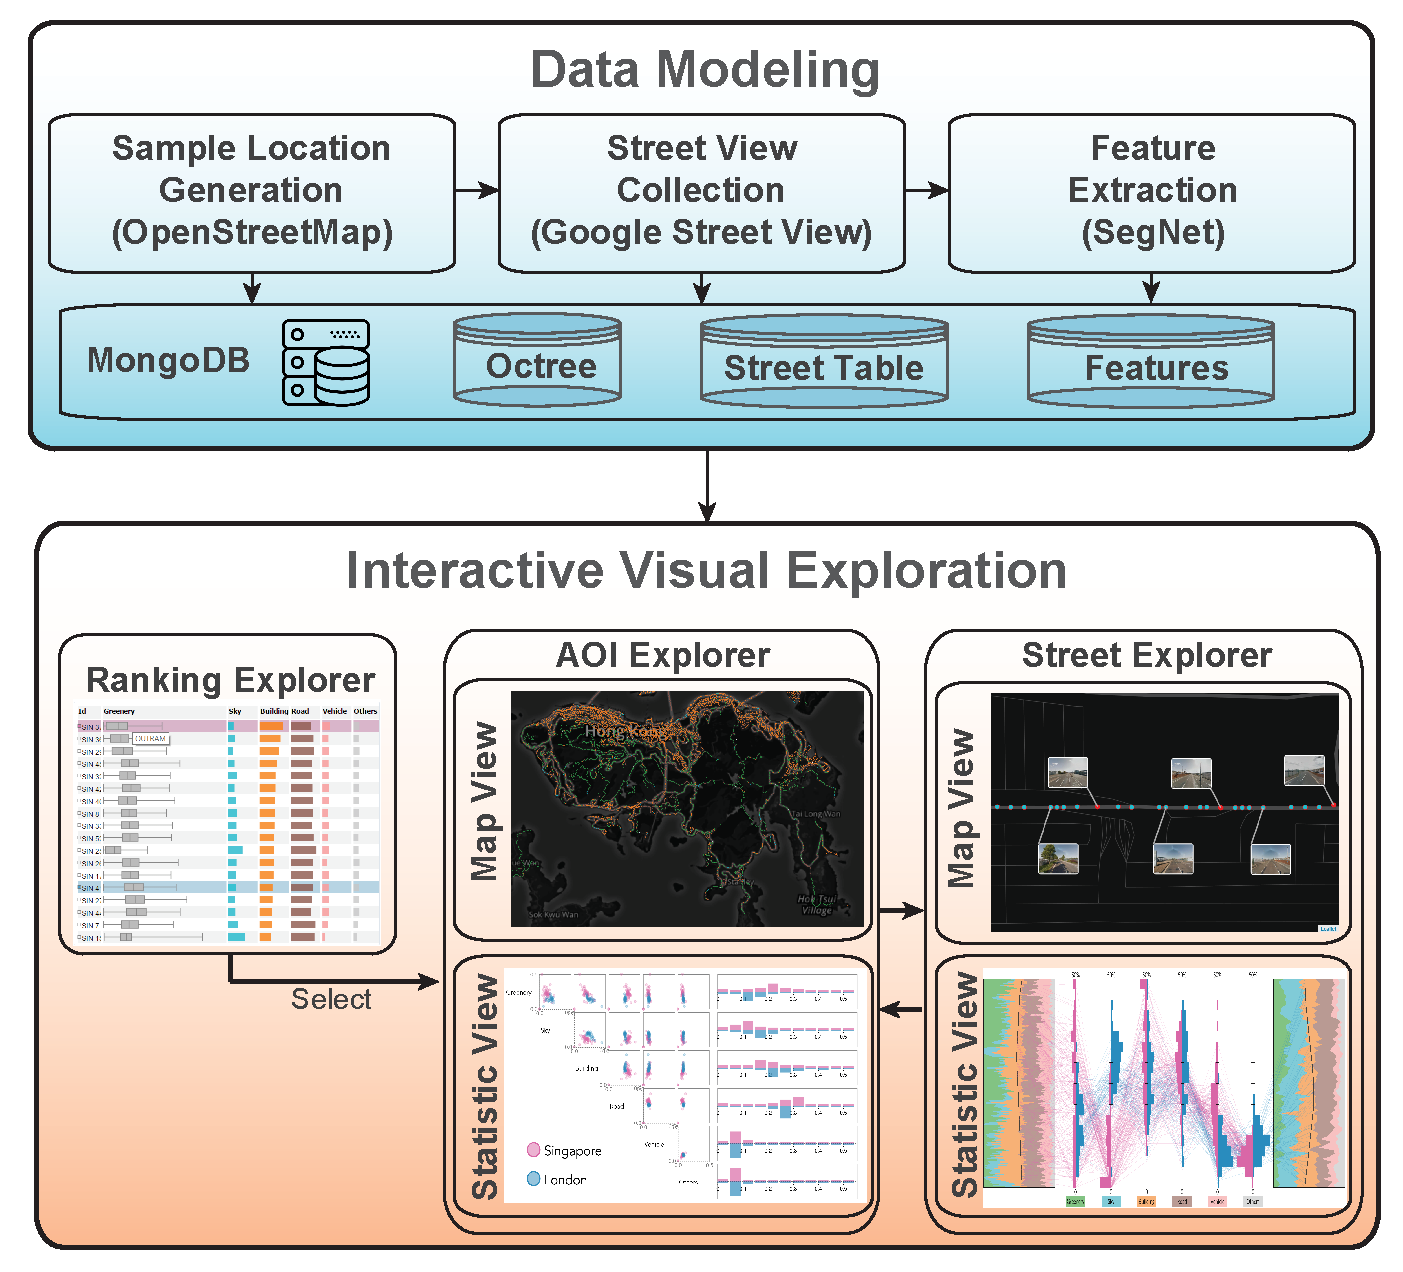
\includegraphics[width=0.9\columnwidth]{figure/streetvizor/fig2_framework/framework}
	\vspace{-5mm}
	\caption{Overview of StreetVizor workflow. Our system consists of two phases: data modeling and interactive visual exploration.}
	\label{fig:c1_sys_overview}
	\vspace{-6mm}
\end{figure}

StreetVizor is a web-based application comprising two major phases, as illustrated in Fig.~\ref{fig:c1_sys_overview}.
In the data modeling phase, our system automatically collects hundreds of thousands of GSV images at sampling positions in each city generated from OpenStreetMap (OSM) (Section~\ref{ssec:c1_data_collection}).
Then, we classify the pixels of the collected images into 12 classes using SegNet, and extract the desired feature metric from the classification results (Section~\ref{ssec:c1_feature}).
Data collection and preprocessing are conducted offline on a high-performance workstation with 12 core 3.40 GHz Intel Core i7-6800K CPU and a GeForce GTX 1080 graphics card.
Though enabled with GPU acceleration, the computation still takes several to 20 hours to preprocess images from each city.
Then, we construct data structures, including an octree and a lookup table, to facilitate visual exploration, such as spatial query and filtering (Section~\ref{ssec:c1_query}).
The datasets are stored in a back-end MongoDB server with 2.4 GHz Intel Xeon E5-2620 CPU and 64 GB memory.

The interactive visual exploration phase consists of two stages:
1) Our system provides users with a Ranking Explorer that ranks and compares multiple AOIs/streets based on human-scale urban forms.
Users can narrow down exploration by selecting two AOIs/streets for detailed comparison. 
2) If two AOIs are selected, the system will present an AOI Explorer that compares the differences in human-scale urban forms in two AOIs at city- and region-scales.
The AOI Explorer is composed of CMVs, including two juxtaposition map views for spatial exploration and a superposition statistic view for comparing various quantitative measurements, such as feature correlations and diversities.
Users can further navigate down to select two streets, and our system will provide Street Explorer, which presents the fine details of human-scale urban forms at street-level.
In Street Explorer, we present map views that show the geographical information and representative images of two streets.
We also develop a novel PCP enhanced with themeriver along street layouts, allowing users to compare multivariate features and reveal feature distributions along the two streets.
The visualization modules are implemented in D3.js and Three.js for different rendering requirements, and they are integrated using Vue.js.

\if 0

. Whole system framework is shown in the figure.2.
The whole system pipeline starts from the data process models. Data process model will collect and analysis Google street view images, mark them with gps tags and generate the human-scale feature vector automatically . The output of the human-scale features with gps information will be stored by mongodb, a nosql database, the correponding geographical index will be generated to improve query speed. Based on mongodb, we build web server with Python/Flask, and Frontend system with Vuejs. The viusalization module are implemented by D3 and Three.js for different render requirement.

The visualization module consists of tow major view: navigation view and analysis view. Navigation view provides high level overview of the human-scale feature distribution as well as many flexible query methods. Users can navigate from different level in the navigation view, to find the analysis target or narrow down to a smaller scope, e.g. a smaller subset of streets or regions. For the selected units, users can conduct an find granularity analysis...

\fi
\section{Data Modeling}
In this section, we first describe the collection of GSV images and the extraction of human-scale urban forms from the collected images.
Furthermore, we present the methods for data querying and filtering.

\begin{figure}[t]
	\centering
	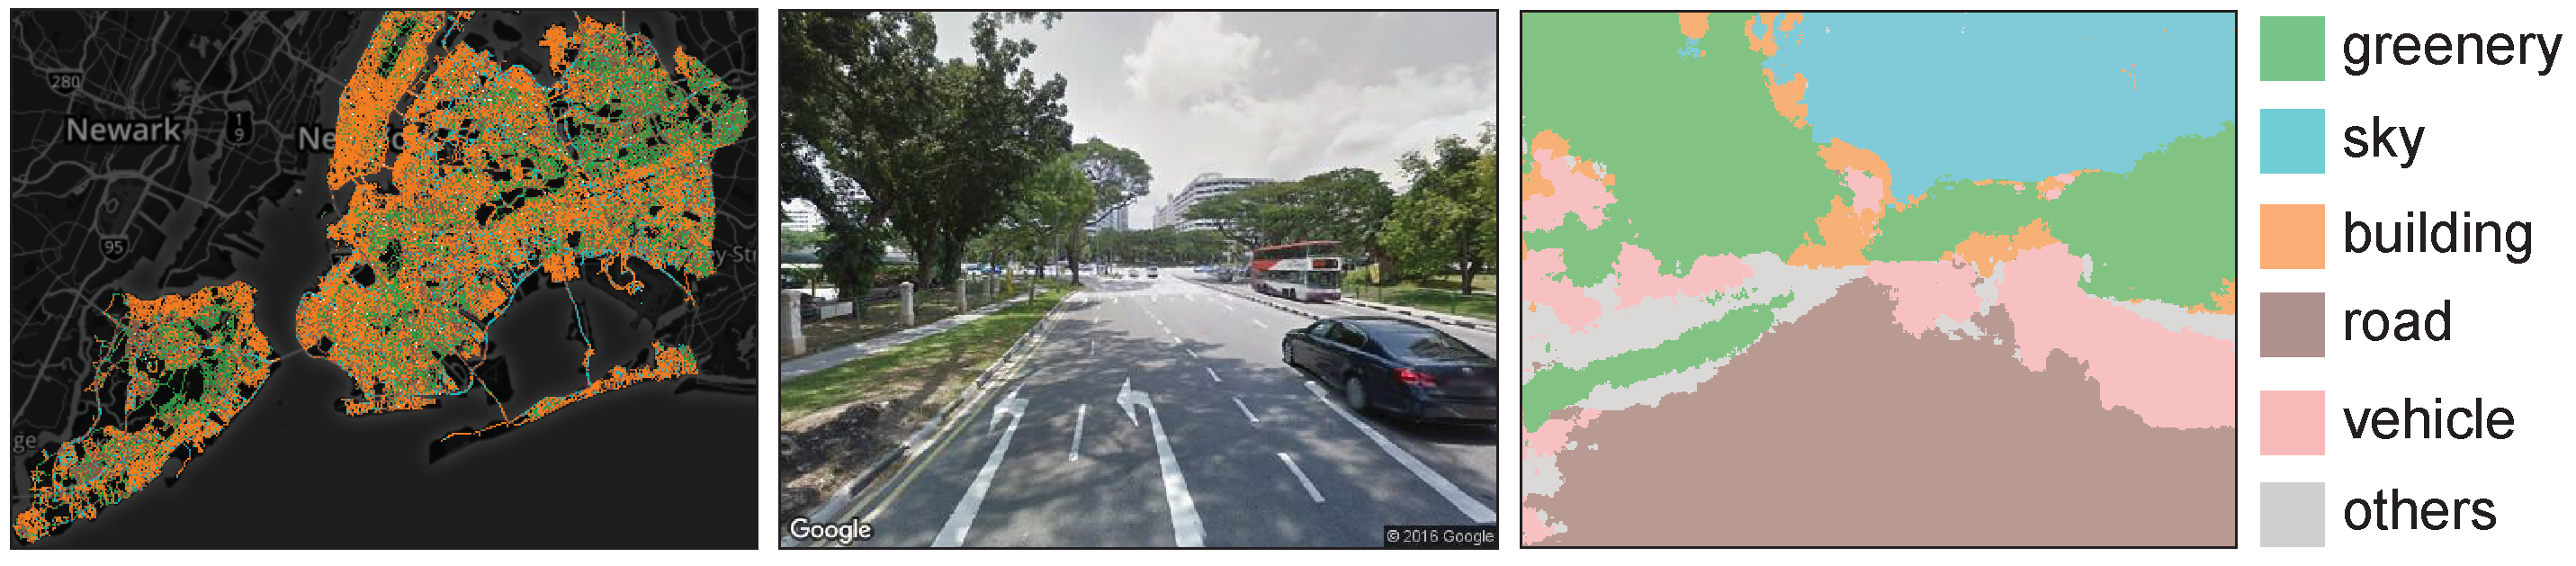
\includegraphics[width=\columnwidth]{figure/streetvizor/fig3_data_preprocess/data_process}
	\vspace{-7mm}
	\caption{Illustration of data preprocessing: sampling locations in New York City are generated from OpenStreetMap (left), a street view image is collected from Google Street View (center), and the image pixels are classified into six features using SegNet (right).}
	\label{fig:c1_data_preprocess}
	\vspace{-4mm}
\end{figure}

%===============================================
\subsection{Data Collection}
\label{ssec:c1_data_collection}

Based on the configurations defined in Section~\ref{sec:c1_bg}, we develop an automatic approach to collect GSV images.
We first download the area of a city from OSM~\cite{osm_api} and extract the road network from the OSM data.
Next, we apply a flood-fill algorithm that recursively goes through the entire road network every 50 meters, starting from a randomly selected location.
After this operation is completed, a list of sampling locations (\{$pos$\}) with geographic information $(lat \; \& \; long)$ is generated.
We then pass each $(lat \; \& \; long)$ into GSV API, and extract the corresponding street information $(SI)$, including street name $(s\_name)$ and heading $(h)$. 
Finally, we download front and back images at each sampling position by passing $lat, \; long \; \& \; h$ with the default field of view and pitch values into GSV API.
Together with the downloaded image ($Img$), we model urban forms at human-scale ($UF_{hs}$) at each sampling location as: 

\vspace*{-2mm}
\begin{equation}
\label{c1_eq_sv}
UF_{hs} \; := \; <pos, \; SI, \; Img>
\end{equation}

We have collected $\sim$147 k, $\sim$183 k, $\sim$685 k and $\sim$637 k images of Hong Kong, Singapore, Greater London and New York City, respectively.
Fig.~\ref{fig:c1_data_preprocess} (left) presents all sampling locations (colored dots) in New York City generated from OSM, and (center) shows a sample street view image downloaded from GSV.

%===============================================
\subsection{Feature Extraction}
\label{ssec:c1_feature}
After collecting street views, we first classify the image pixels into 12 classes (e.g., sky and building) using SegNet~\cite{Badrinarayanan_2015_segnet}, which is a robust pixel-wise semantic labeling tool with a global accuracy of 82.8\%.
Among the 12 classes, we count the number of pixels for the identified five features, i.e., $greenery$, $sky$, $building$, $road$, and $vehicle$, and summarize the remaining pixels as $others$.
We then normalize the feature data because pixel counts ($PC$) as raw output values are not intuitive.
The normalization is straightforward for each feature value ($FV$):
$ FV_i \; = {PC_i} / {PC_{Img}} $, where $i \in \{g, s, b, r, v, o\}$ represent the five features and $others$.
Hence, all feature values are in the range of [0, 1].
Then, we can replace the image ($Img$) with a feature metric ($FM$) as:

\vspace*{-2mm}
\begin{equation}
\label{c1_eq_fm}
Img \rightarrow FM := \; <FV_g, \; FV_s, \; FV_b, \; FV_r, \; FV_v, \; FV_o>
\end{equation}

% The feature extraction is preprocessed on a high-performance workstation with GTX 1080 graphics card. 
% Though enabled with GPU acceleration, the computation still takes from several to up to 20 hours to process the images in each city.
Fig.~\ref{fig:c1_data_preprocess} (right) shows the classification result of the street view image in the center produced by SegNet.

%===============================================
\subsection{Data Querying and Filtering}
\label{ssec:c1_query}

Based on Equations~\ref{c1_eq_sv} and~\ref{c1_eq_fm}, we model human-scale urban forms ($UF_{hs}$) with the following attributes: position ($pos$), street information ($SI$), and feature metric ($FM$).
By nature, the data exhibits the following properties: 
1) $spatial$, i.e., positions;
2) $multi$-$scale$, because the positions can be hierarchically grouped in accordance with city and regional units, or street information;
and 3) $multivariate$, i.e., the feature metric is in six-dimensional data space.

These complex data natures bring in challenges for our analytical tasks.
To address these challenges, we further identify the following querying and filtering models that our system should support:

\vspace*{-2mm}
\begin{itemize}

\item
\textbf{Spatial Query}:
To overview the feature distributions within an AOI (T.1.1), our system should first support an efficient query of a list of \{$UF_{hs}$\} with their $pos$ laying in a given AOI.
The AOI can be either an administrative zone (e.g., a city or a district) or a user-specified region defined using a lasso tool.
We achieve the efficient spatial query operation by organizing all \{$UF_{hs}$\} in a city in a four-level octree structure, in which the topmost level is the boundary of each city.

\vspace*{-2mm}
\item
\textbf{Street Query}:
To support the exploration of human-scale urban forms at street-scale (T.1.2), our system should allow users to interactively query a street by its name.
Here, we create a lookup table with street names as keys, and store corresponding $UF_{hs}$ ids in each street slot.

\vspace*{-2mm}
\item
\textbf{Feature Filtering}:
To accelerate filtering against a particular feature (T.2.2), our system first sorts all \{$UF_{hs}$\} to be explored in increasing order for every feature.
Then, we adopt a binary search approach in run time.

\end{itemize}

%===============================================
\begin{figure}[t]
	\centering
	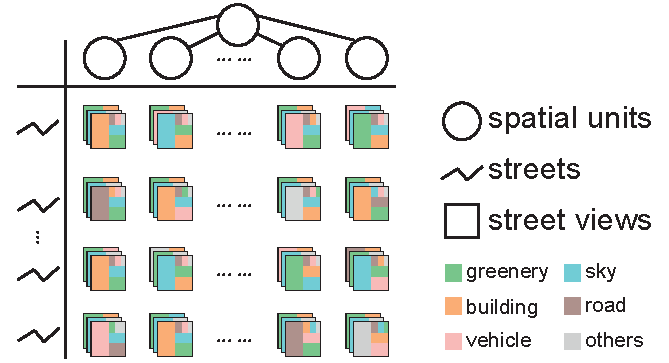
\includegraphics[width=0.8\columnwidth]{figure/streetvizor/fig4_data_model/data_model}
	\vspace{-3mm}
	\caption{Data model: street views with six-dimensional features of \textit{greenery, sky, building, road, vehicle} and \textit{others}, are organized in an octree structure and a street lookup table.}
	\vspace{-5mm}
	\label{fig:c1_data_model}
\end{figure}

\vspace*{-2mm}
Fig.~\ref{fig:c1_data_model} illustrates the data model that organizes the street views in an octree structure and a street lookup table.
Each street view contains the six-dimensional features of \textit{greenery, sky, building, road, vehicle}, and \textit{others}.
We store these querying and filtering models are stored in a back-end MongoDB database, as shown in Fig.~\ref{fig:c1_sys_overview}.
%===============================================

\section{Visualization Design}

In this section, we first discuss the rationales behind our visualization design. 
Then, we provide a detailed description of the visualization techniques implemented in our system.

%============================================================== Teaser

\begin{figure}[t] 
	\centering
	% \vspace{-4mm}
	\includegraphics[width=0.9\columnwidth]{figure/streetvizor/fig1_teaser/teaser}
	\vspace{-3mm}
	\caption{StreetVizor system. 
		(a) Control panel enables multi-scale navigation, ranking exploration, and feature filtering.
		(b) Side-by-side map views compare the spatial distribution of human-scale urban forms in two areas-of-interest (AOIs).
		(c) AOI statistic view presents the quantitative measurements, including correlation, histogram, and diversity in the AOIs shown in (b).
		(d) Street map views present detailed street views along two streets.
		(e) Street statistic view extends parallel coordinates with street layouts.}
	\label{fig:c1_teaser}
	\vspace{-5mm}
\end{figure}


%==============================================================

\subsection{Design Rationales}
To address the complex analytical tasks (Section~\ref{ssec:c1_tasks}), a proper visual design should follow the design rationales below:

\begin{enumerate}[label={R.\arabic*:}]

\vspace*{-2mm}
\item
\textbf{Overview+Details}:
To facilitate multi-scale exploration, our system should follow the information-seeking mantra: ``Overview first, zoom and filter, then details on demand"~\cite{shneiderman1996eyes}.
First, the system should provide an overview of human-scale urban forms at city- and region-scales, and then allow users to explore more details at street-scale.
Efficient query and filtering should be provided to enable smooth transitions between these scales.

\vspace*{-2mm}
\item
\textbf{Coordinated Multiple Views}:
Our system should effectively reveal multiple perspectives information of human-scale urban forms, including geographical locations and multivariate features.
CMVs that present linked information and allow users to explore data from multiple joint-perspectives fulfill this requirement.


\vspace*{-2mm}
\item
\textbf{Effective Comparison}:
To enable effective data comparison, different comparative visualization techniques should be employed for multiple-perspective information.
Specifically, given that spatial information for two AOIs/streets is unsuitable for direct overlay, we adopt side-by-side map views.
On the other hand, the feature metric can be mapped on the same scope. 
Therefor, we select a superposition visualization to reveal the differences.

\vspace*{-2mm}
\item
\textbf{Visual Consistency}:
Since multi-scale and multiple-perspective visualizations are to be designed, the system should maintain visual consistency across different visualization modules.
We realize visual consistency by 
1) applying the same layout, i.e., presenting spatial information on the top and quantitative measurements on the bottom, in AOI Explorer and Street Explorer;
2) employing consistent color mappings. 
Specifically, we set green, light blue, orange, brown, light pink, and gray to represent the features of $greenery$, $sky$, $building$, $road$, $vehicle$, and $others$, respectively.
AOIs/streets on the left and right side are colored as red and blue, respectively.

\end{enumerate}

%==============================================================
\subsection{Ranking Explorer}
Ranking Explorer is developed to overview feature attributes across multiple AOI/street candidates to help users quickly identify AOIs/streets for comparison (T.3.1).
The explorer presents each candidate as a row and arranges its multivariate information in seven columns.
The first column provides general information, such as city and region/street id. 
The remaining columns present the six features' mean values as bars, where mean values are normalized and encoded by bar lengths.
Clicking the body of a feature column of interest will expand the column as a boxplot to show statistical distributions.
The explorer also allows users to sort candidates against a particular feature and the ranking will update correspondingly.
Such designs have been well established and evaluated in a previous work~\cite{liu_2017_smartAdP}.

Fig.~\ref{fig:c1_teaser}(a) ranks all districts in Hong Kong in accordance with $building$ feature (red dashed box).
As an example, we observe the detailed statistics of the $sky$ feature.
We select the column for this feature and expand it to boxplot. 
By comparing the orderings of $greenery$, $sky$, and $building$ features, we find $greenery$ and $sky$ features are correlated, while they are negatively correlated with the $building$ feature.
This information helps users narrow down the comparison choices to 1) district HK 16 (Yau Tsim Mong) with the highest $building$ ratio and 2) district HK 7 (Sai Kung) with low $building$ and high $greenery$ ratios, as shown in Figs.~\ref{fig:c1_teaser}(b) \& (c).
% We also find one special region HK 0, which is Central and Western, has both high green feature and building feature. 
% In addition, there is also some street in this region has very high sky feature value. This region could provide a relative good work environment.

% \qm{Even though query methods can effectively help to narrow down to a small scope of AOIs and streets, the planers still need to explore among the small number of candidates. The quantitative ranking and comparison tools based on different features are required for the planers to explore more than two candidates}.
% \qm{The interactions above enable users to narrow down the study scope to several candidates AOIs or streets. To further explore the and find the interested  candidates, we implemented multi-features exploration view (Fig.~\ref{fig:teaser}(a)) which enable quantitative ranking and compare multiple AOIs and streets based on the features interested. Inspired by Lineup~\cite{gratzl2013lineup} and SmartAdp~\cite{liu2017smartadp}, each column indicates one attribute of the AOI/street. The last 6 columns present the six human scale features while other columns present other properties like the id, city they belong to, which can be interactively chosen according to the users' interests. Users can also click on the head to rank the candidates according to the specific features or group several features and rank the candidates by the sum of the selected features.}
%==============================================================
\subsection{AOI Explorer}
\label{ssec:c1_aoi_explorer}
AOI Explorer is developed to provide efficient comparison of human-scale urban forms at city- and region-scales (T.1.1).
The explorer integrates coordinated multiple views, including:

%============================
\subsubsection{AOI Map View}
\label{sssec:c1_aoi_map_view}

We develop side-by-side map views (Figure.~\ref{fig:c1_teaser}(b)) to compare the spatial distributions of human-scale urban forms in two AOIs (T.3.2).
Each map view consists of:
1) a background map layer implemented with Leaflet.js to allow users to change map style (e.g. satellite, street, and sport) for different purposes;
and 2) a point density map overlaid on top of the background map layer, with points representing street views.
The density points are evenly sampled on each street with an upper limit of 10,000 points.
Point color corresponds to the maximum feature value in the street view image.
A corresponding street view image will pop up when the mouse pointer hovers over a point.
Users can select two cities or regions from the navigation panel, or directly manipulate AOIs on the map views with a lasso tool.

Heat map is an alternative design for the point density map.
However, in this work, we focus on the simultaneous analysis of multiple features of human-scale urban forms.
Compositing these features into one heat map~\cite{scheepens_2011_composite} will require redundant user interactions.
In addition, sampling positions are generated along the street network.
Thus, no street views is collected from many places across a city.
In this case, the heat map will generate ambiguity between the two scenarios of 1) no record or 2) low feature values in a region.

\begin{figure}[t]
	\centering
	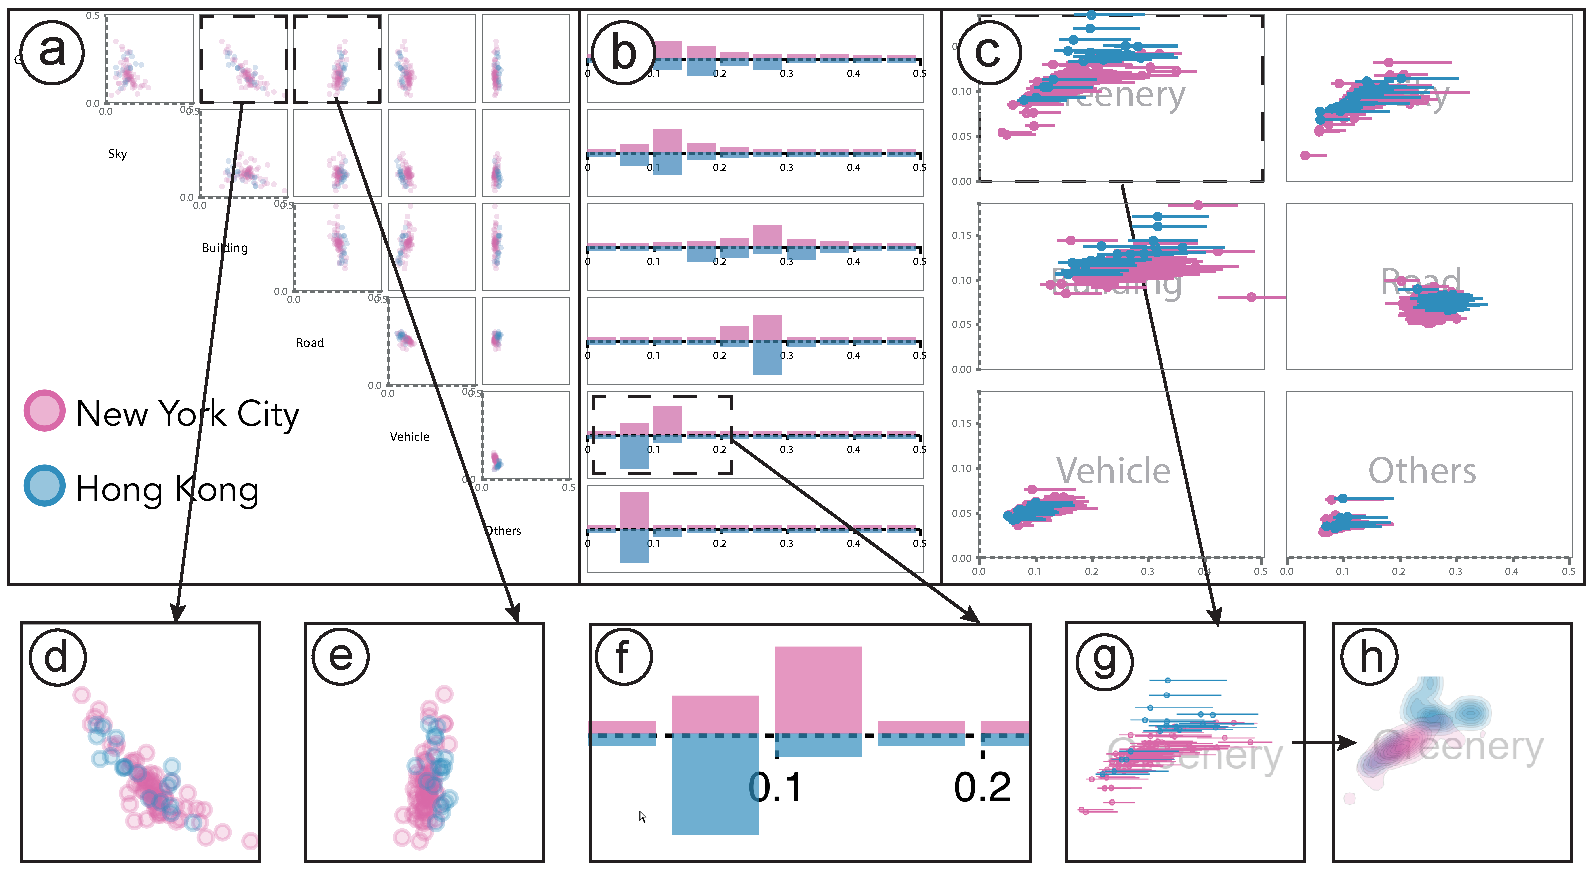
\includegraphics[width=0.85\columnwidth]{figure/streetvizor/fig5_statistic_view/statistic_view}
	\vspace{-4mm}
	\caption{The AOI Statistic View combines (a) a scatterplot matrix to show pair-wise correlations between two features, (b) small multiples of histogram bar charts to overview feature distributions, and (c) small multiples of deviation plots to present feature diversity. }
	\label{fig:c1_statistic_view}
	\vspace{-4mm}
\end{figure}

%============================
\subsubsection{AOI Statistic View}
\label{sssec:c1_statistic_view}
Besides the map view, which enables the comparison of spatial distributions of human-scale urban forms, we develop AOI Statistic View to allow users to compare various quantitative measurements (T.3.3).
Nonetheless, each AOI may contain too many street views (up to several hundred thousand) that will overload the rendering process.
Moreover, the street views will occlude each other if we simply plot all of them.
To address this problem, we cluster street views into groups based on either their administrative units (districts, divisions, and streets) or a mean-shift clustering algorithm~\cite{comaniciu_2002_meanshift} that works as follows.
 
\vspace*{2mm}
\noindent
\textbf{Mean Shift Clustering}.
We cluster urban forms based on their feature metric and geographical positions.
Our algorithm works in the following way: 
given an input list of $N$ human-scale urban forms \{$UF_{hs}$\}, we first normalize the $lat$ \& $long$ attributes of each $UF_{hs}$ against the boundary of all \{$UF_{hs}$\}.
Then, we combine the normalized $lat_{nor}$ \& $long_{nor}$ with the feature metric to construct a new dataset $X := \{x_1, x_2, ..., x_N\}$, where each data point $x_i$ is in an eight-dimensional space, $R^{8} := \; <lat_{nor}, \; long_{nor}, \; FV_g, \; FV_s, \; FV_b, \; FV_r, \; FV_v, \; FV_o>$.
The distance between two data points is measured as their Euclidean distance.
We then estimate a bandwidth $h$ from $X$, and apply mean-shift clustering algorithm on $X$ using a flat kernel.
Here, the bandwidth estimation and mean shift clustering are performed with a machine learning library \textit{scikit-learn}~\cite{scikit-learn}.
Finally, we generate a list of $m$ urban form clusters $C := \{c_1, c_2, ..., c_m\}$, where each cluster $c_i$ contains $n$ data point $c_i := \{x_1, x_2, ..., x_n\}$.

The clustering process groups geographically close street views with similar feature attributes together.
Given that locations are integrated as two-dimensional spaces, the algorithm forms more local clusters than an algorithm without considering spatial information, which usually generates several big clusters with too many street views.
The algorithm may be further improved by adopting a network-based distance measurement approach other than Euclidean distance.
We expect to form more representative clusters of street views with street network information.
Nonetheless, the current approach fulfills our requirement of reducing visual clutter.

\vspace*{2mm}
After generating the clusters $C$, we further compute and visualize the following quantitative measurements:

\vspace*{-2mm}
\begin{itemize}

\item
\textbf{Feature Correlation}:
We first compute the mean values of the identified features, i.e., \textit{greenery, sky, building, road, vehicle}, and \textit{others} in each cluster $c_i$.
We then plot the pair-wise correlations using a scatterplot matrix (Fig.~\ref{fig:c1_statistic_view}(a)).
Notice that the clusters in the left and right AOIs are colored red and blue, respectively.

\vspace*{-1mm}
\item
\textbf{Feature Histogram}:
Though feature values fall in the range of [0\% - 100\%], we seldom find feature values that exceed 50\%.
Thus, we only consider the range [0\% - 50\%].
For each feature, we divide the range into 10 even parts, i.e., [0\% - 5\%), [5\% - 10\%)..., and aggregate the corresponding value in each street view to each part.
Then, histograms for each feature are plotted as bar charts in an up and down manner for AOIs on the left and right, respectively.
The six histogram bar charts are arranged in small multiples next to the scatterplot matrix (Fig.~\ref{fig:c1_statistic_view}(b)).

\vspace*{-1mm}
\item
\textbf{Feature Diversity}:
We use standard deviation to indicate the measured feature diversity measured for each cluster, and design diversity views that are arranged as six side-by-side small multiples for each feature as shown in Figure~\ref{fig:c1_statistic_view}(c).
In every feature diversity view, each cluster is represented as a dot with its x-value indicating the averaged feature value and y-value indicating standard deviation.
In addition, we use line segments to indicate the largest and smallest feature values in each cluster. 
In case an AOI may have hundreds of clusters that lead to serious visual clutter problem, we implement a contour map view~\cite{chen_2014_visual} (Fig.~\ref{fig:c1_statistic_view}(h)) to show overall distribution patterns.
Users can interactively choose one of the views in accordance with different requirements.

\end{itemize}

The AOI Statistic View comparison of New York City (red) and Hong Kong (blue) is shown in Fig.~\ref{fig:c1_statistic_view}.
From the view, we can easily identify some obvious patterns.
For example, in both cities, \textit{greenery} and \textit{building} features are negatively correlated (Fig.~\ref{fig:c1_statistic_view}(d)).
The correlations between other pairwise features, e.g., \textit{greenery} and \textit{road} (Fig.~\ref{fig:c1_statistic_view}(e)), are not obvious.
From Fig.~\ref{fig:c1_statistic_view}(f), we find that the vehicle ratio is higher in New York City than in Hong Kong.
In addition, we find that although the \textit{greenery} values are similar for both cities, diversity is higher in Hong Kong (Fig.~\ref{fig:c1_statistic_view}(g)).
This results reflects that greenery is better integrated into street space in New York City than in Hong Kong.

%==============================================================
\subsection{Street Explorer}
\label{ssec:c1_street_explorer}

\begin{figure}[t] 
	\centering
	% \vspace{-4mm}
	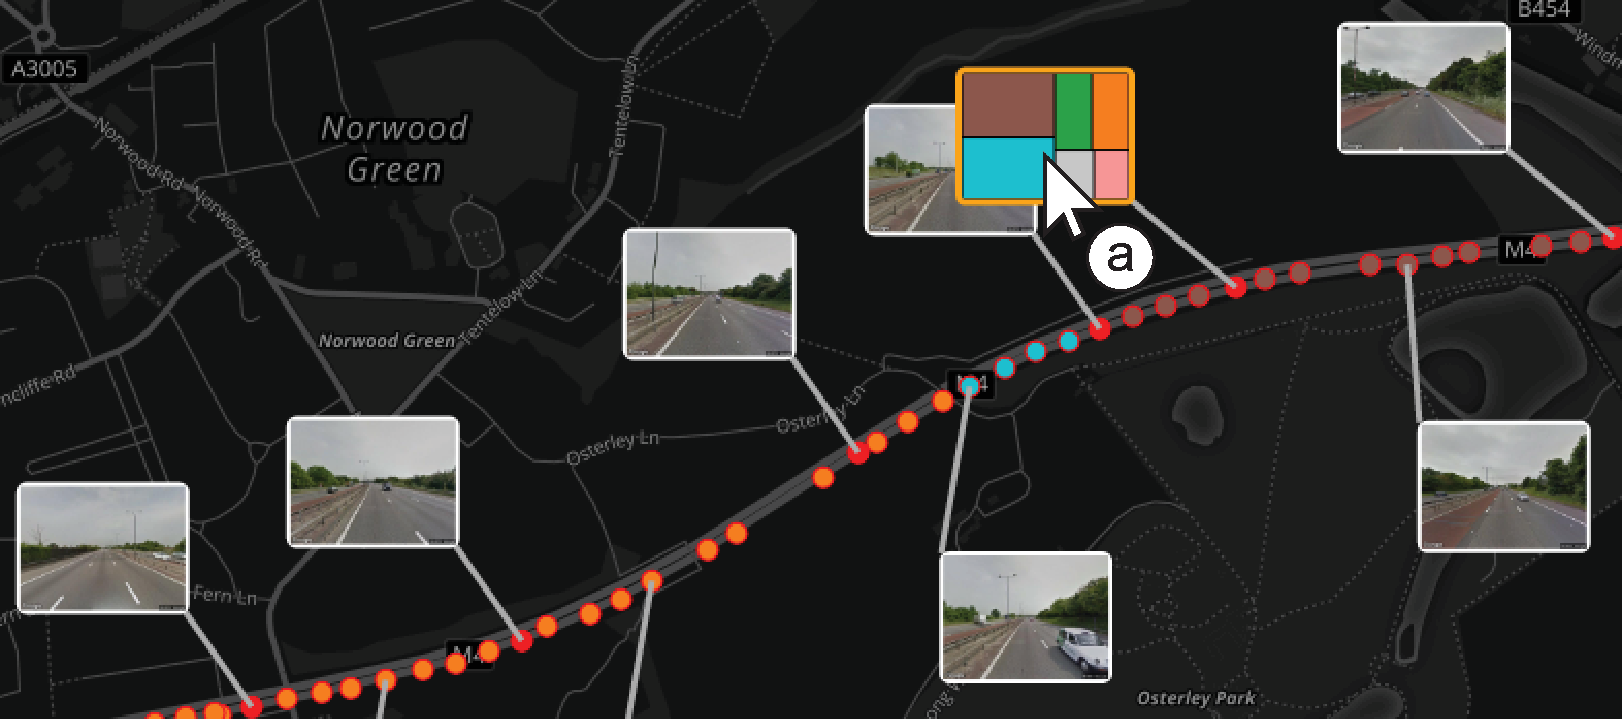
\includegraphics[width=0.9\columnwidth]{figure/streetvizor/fig6_street_map_view/street_map_view}
	\vspace{-3mm}
	\caption{Street Map View provides an overview of all street views along a street as colored points, and highlights images on two sides of the street.
	(a) A tree map showing the feature composition of an image will pop up when the mouse pointer is hovered over the image.}
	\label{fig:c1_street_map}
	\vspace{-5mm}
\end{figure}

%============================

Street Explorer is developed to enable the efficient comparison of human-scale urban forms at street-scale (T.1.2). 
The explorer adapts the same layout as that in the AOI Explorer, i.e., juxtaposition map views are placed on the top of the explorer, whereas detailed statistics view are on the bottom. 

\subsubsection{Street Map View}
\label{sssec:c1_street_view}

Similar to AOI Map View, Street Map View is also developed on top of a background map layer that is implemented using Leaflet.js.
Street views on the street are over-viewed as points with colors that correspond to primary features, i.e., green for $greenery$, light blue for $sky$ and orange for $building$.
In contrast to AOI Map View, Street Map View presents more details of human-scale urban forms by displaying the corresponding street view images along the two sides of a street.
The images are evenly selected in the direction of the street heading. 
In particular, the feature compositions of an image are displayed as a tree map~\cite{shneiderman_1992_tree} when users hover their mouse pointer over the image.
An example is provided in Fig.~\ref{fig:c1_street_map}(a).

%============================

\subsubsection{Street Statistic View}
\label{sssec:c1_street_stat_view}

The design goal for this view is to allow users to quantitatively compare human-scale urban forms from two streets.
Although we can utilize the same views shown in the AOI Statistic View, our collaborating domain expert $SR$ is not satisfied.
$SR$ strongly recommended encoding street layout information in the view, so that users can better leverage their knowledge about streets to perform in-depth analysis.
$SR$ felt the spatial information was not well integrated with the Street Map View.

Based on this goal, we experimented with a few alternative designs and informally evaluated design prototypes with $SR$.
For our first prototype, we designed some glyphs, such as a radial chart or tree map, and directly overlaid the glyphs on the map view.
The design was aborted because isolating statistics on the two maps weakened the effects of comparison.
In addition, such a design easily generated visual clutter, which requires redundant user interactions or clustering to address.
For the second prototype, we encoded street layout information in a similar design as the AOI Statistic View.
However, this method was extremely difficult because the rendering space was fully utilized. 

\begin{figure}[t]
	\centering
	\includegraphics[width=0.9\columnwidth]{figure/streetvizor/fig7_street_model/street_pcp}
	\vspace{-5mm}
	\caption{Overview of the construction process for Street Statistic View:
	(a) Construct minimum bounding box of the street network.
	(b) Rotate the street network such that its bounding box fits in the rendering space.
	(c) Plot themeriver style visualization within the rendering space.
	(d) Enhance parallel coordinates with street layouts on both sides.}
	\label{fig:c1_street_statistic_view}
	\vspace{-6mm}
\end{figure}

\vspace*{2mm}
\noindent
\textbf{PCP with Street Layout}. Inspired by~\cite{qu_2007_visual}, we ultimately develop a design of a parallel coordinates enhanced with street layouts (Fig.~\ref{fig:c1_street_statistic_view}(d)).
We elaborate the construction of this design as follows:

\vspace*{1mm}
\noindent
\textit{Bounding Box Construction} (Fig.~\ref{fig:c1_street_statistic_view}(a)).
The first step is to construct a minimum bounding box ($MBB$) of the street layout.
% , which is represented as lines connecting positions of corresponding street views.
We find the starting ($A$) and ending ($B$) points, and generate a primary axis pointing from $A$ to $B$.
$MBB$ is generated as the minimum rectangle that contains all nodes of the street network parallel with the primary axis.

\vspace*{1mm}
\noindent
\textit{Street Layout Rotation} (Fig.~\ref{fig:c1_street_statistic_view}(b)).
Next, we rotate the street layout such that $MBB$ fits in the rendering space, i.e., $A$ and $B$ lay on the top and bottom (or vice versa) sides of the rendering space, and the rotated $MBB$ lays in the center.
In the case that $MBB$ is wider than the rendering space, the street layout outside the rendering space is clipped.
The rotation direction (clockwise or anticlockwise) is determined based on the direction that produces the minimum rotation angle.

\vspace*{1mm}
\noindent
\textit{ThemeRiver Plotting} (Fig.~\ref{fig:c1_street_statistic_view}(c)).
To fully utilize rendering space, we plot a themeriver-style~\cite{havre_2002_themeriver} visualization to show changes in feature values along a street layout.
Here, the themeriver is plotted in the vertical instead of the traditionally horizontal direction because the street layout is aligned along the y-axis after rotation.
Next, given that street views are sampled evenly along the street layout, we map the street views equally onto the y-axis, i.e., y-values of the themeriver plot reflects the relative positions of street views along the street layout.

We start plotting the themeriver visualization using the left side of the rendering space as the baseline and calculate the upper bound x-values for the $greenery$ feature.
The upper bound x-values of the $greenery$ layer are then used as baseline values for the next feature, i.e., $sky$.
This process is repeated until all features are plotted.
To support better feature comparison, our system allows users to reorder feature sequence by clicking on the feature layer of interest and shifting it to the left side~\cite{byron_2008_stacked}.

\vspace*{1mm}
\noindent
\textit{PCP Integration} (Fig.~\ref{fig:c1_street_statistic_view}(d)).
The themeriver plot can be used as a coordinate for the PCP.
To enable comparison between two streets, we integrate their themeriver plots into a PCP on left and right sides, and the identified features are used as other coordinates.
Each street view is conveniently presented as a polygonal line, which is colored as red and blue for left and right street views, respectively.
In addition, we aggregate the feature values via binning techniques on left and right sides of each feature coordinate to facilitate the visual comparison of feature distributions.

\vspace*{1mm}
Fig.~\ref{fig:c1_street_statistic_view}(d) presents an example Street Statistic View.
A first glimpse at the two themeriver plots, we can find that the left street contains more $greenery$, while on the right street people can see more $sky$.
This can be found in the distribution comparison on the $greenery$ \& $sky$ coordinates in the middle.
Besides, we can also find that feature values vary dramatically on the left themeriver plot, showing street views are very different along the left street.


\begin{figure}[t]
	\centering
	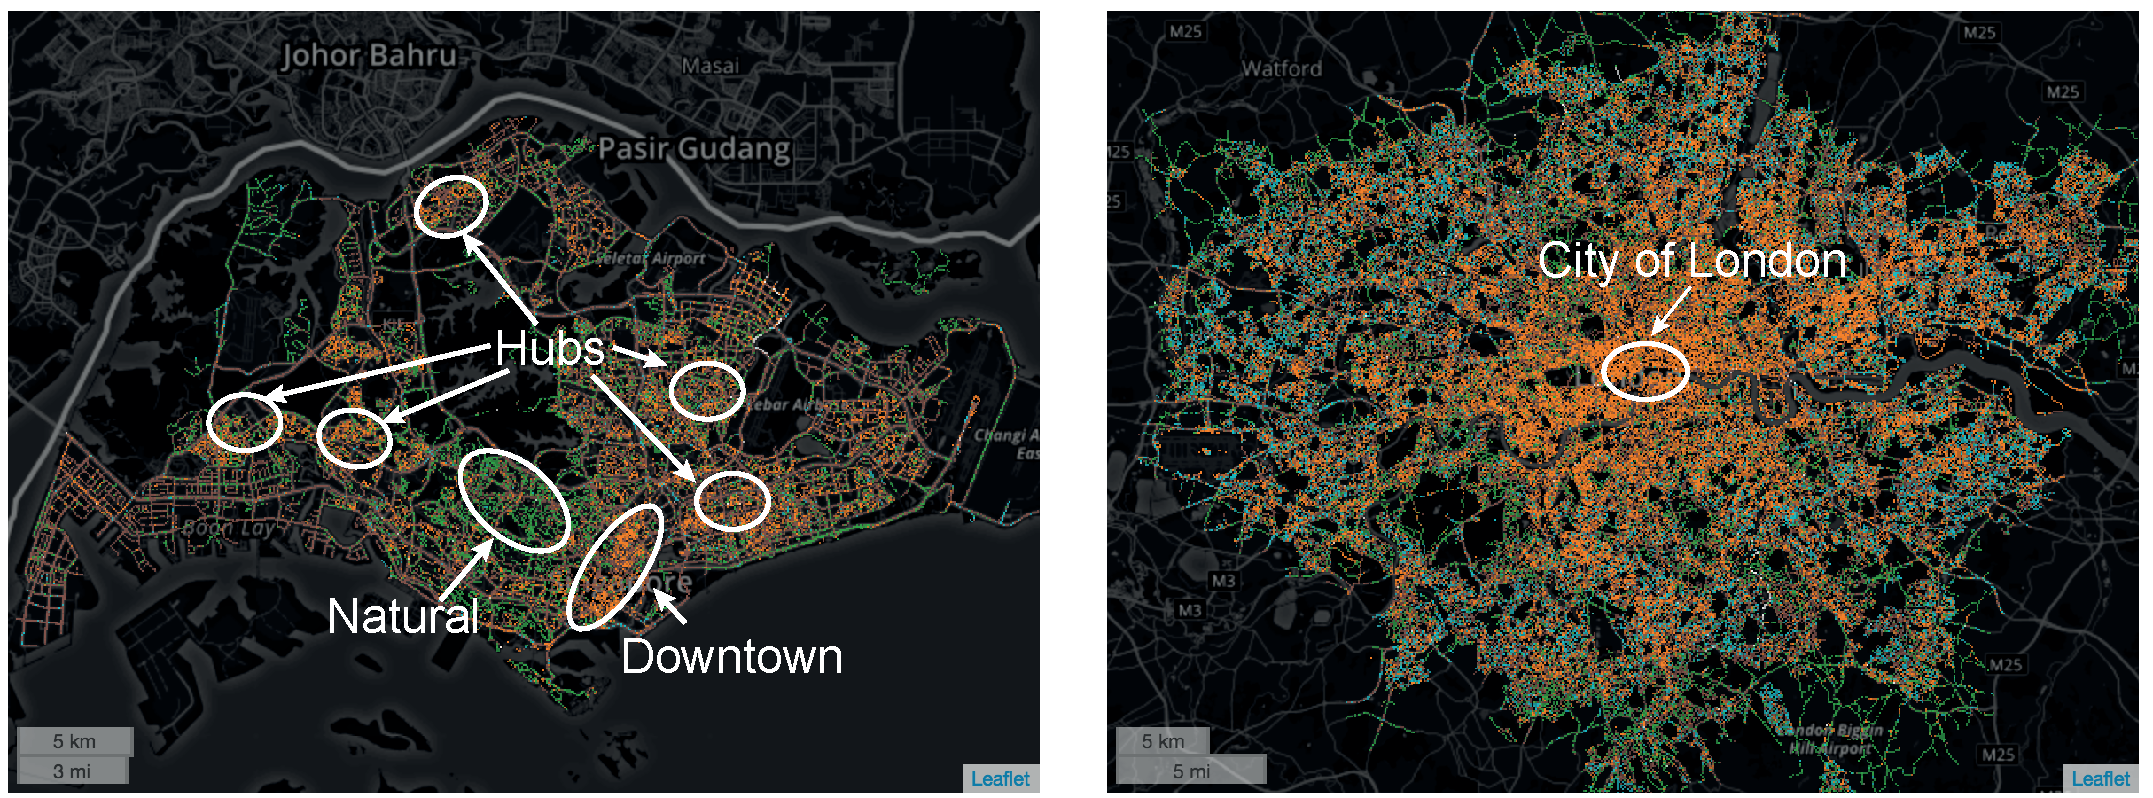
\includegraphics[width=0.95\columnwidth]{figure/streetvizor/fig8_study_1/study_1_spatial}
	\vspace{-4mm}
	\caption{
	AOI Map View compares spatial distributions of human-scale urban forms in Singapore (left) and Greater London (right).
	Orange points (buildings) are concentrated around the highlighted center area of Greater London, i.e., City of London.}
	\label{fig:c1_study_1_spatial}
	% \vspace{-2mm}
\end{figure}

\begin{figure}[t]
	\centering
	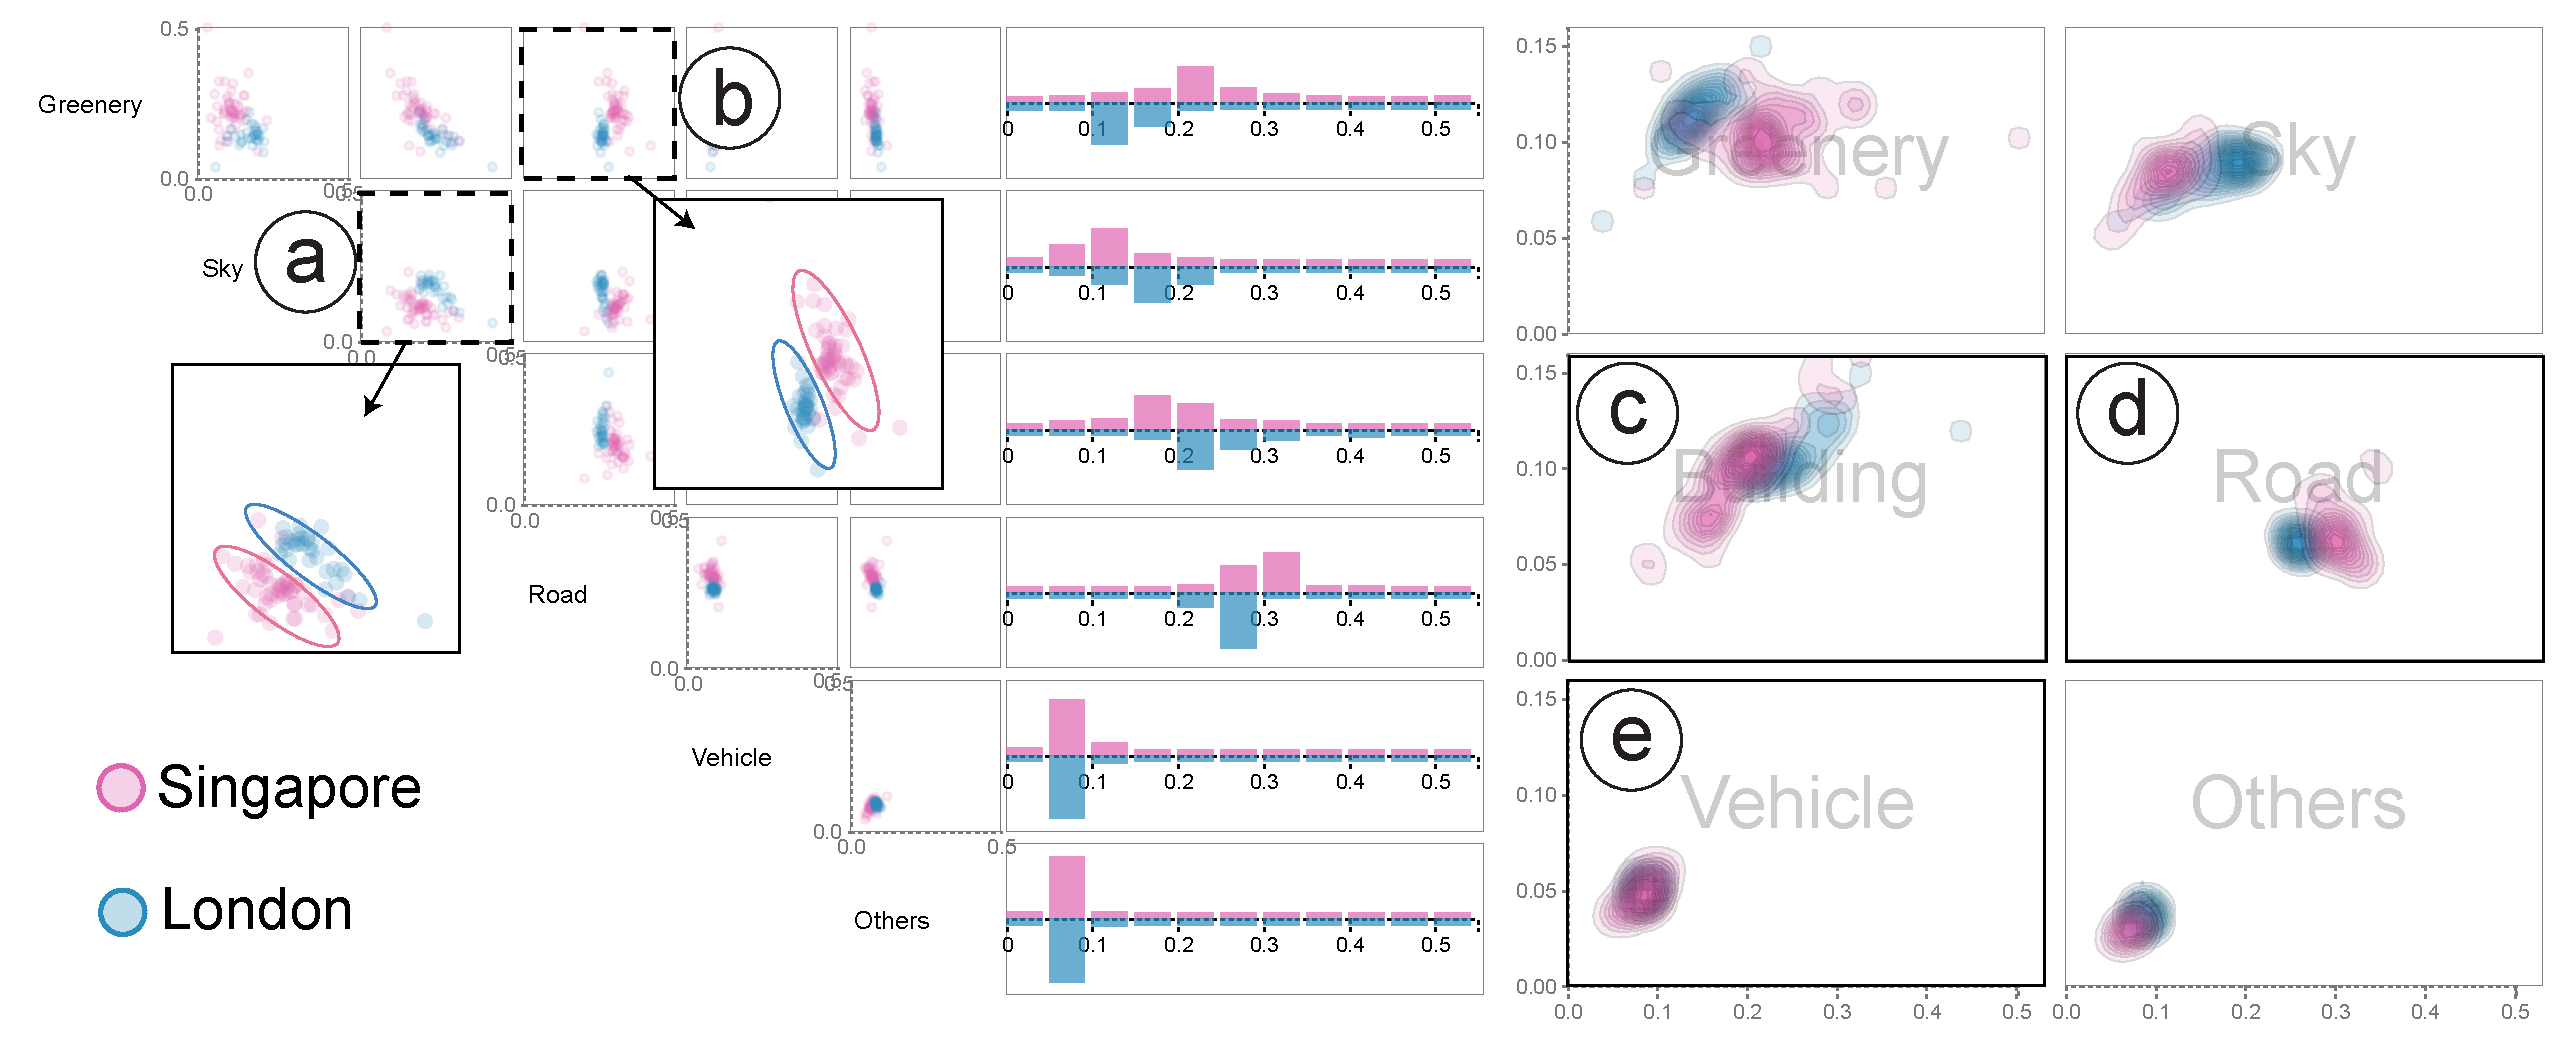
\includegraphics[width=\columnwidth]{figure/streetvizor/fig8_study_1/study_1_statistic}
	\vspace{-7mm}
	\caption{AOI Statistic View in coordination with Fig.~\ref{fig:c1_study_1_spatial} presents quantitative measurements differences of human-scale urban forms in Singapore (red) and Greater London (blue).}
	\label{fig:c1_study_1_statistic}
	\vspace{-5mm}
\end{figure}


%==============================================================
\subsection{User Interactions}
\label{ssec:c1_user_interaction}

\QM{In addition to basic interactions in each view, StreetVizor also provides a control panel (Fig.~\ref{fig:c1_teaser}(a)) that enables:}

\begin{itemize}

\vspace*{-1mm}
\item
\textit{Multi-scale Navigation}.
To help users navigate effectively across different scales, we develop city-, region- and street-panels.
The city-panel lists all four cities, i.e., Hong Kong, Singapore, Greater London, and New York City.
Users start navigation by selecting a city. 
The region-panel will then list all administrative regions under the city.
For instance, City of London and Kingston will be listed if Greater London is selected.
Similarly, the street-panel lists all the streets inside a selected city or region.
% We also provide a region and street query by entering a corresponding name.

\vspace*{-1mm}
\item
\textit{Feature Filtering}.
Our system also supports filtering human-scale urban forms against a specific feature by specifying the value range with feature sliders. 
By default, each feature slide within [0 - 1], and users can change the minimum and maximum values by dragging the slider buttons.

\end{itemize}

In addition, our system also supports the following user interactions to facilitate visual exploration.
\begin{itemize}

\vspace*{-1mm}
\item
\textit{Details on Demand}.
To enable overview+details (R.1), we develop a set of interactions that allow users to explore the details of human-scale urban forms on demand.
For example, if a street view point is selected in the AOI Map View, the corresponding image will show up.
Thus, users can leverage their domain knowledge by visually examining street views.

\vspace*{-1mm}
\item
\textit{Linking}.
Our system supports automatic linking among the visualization modules in both AOI Explorer and Street Explorer for coordination across multiple views (R.2).
For example, if a specific street view on the AOI Map View is selected, the cluster that contains the street view in the scatterplot matrix and the diversity views will be highlighted accordingly.

\end{itemize}
\section{Case Studies}

This section presents three case studies on the application of StreetVizor in assisting urban planners to explore and compare human-scale urban forms on the city-, region-, and street-scales.

\begin{figure}[t]
	\centering
	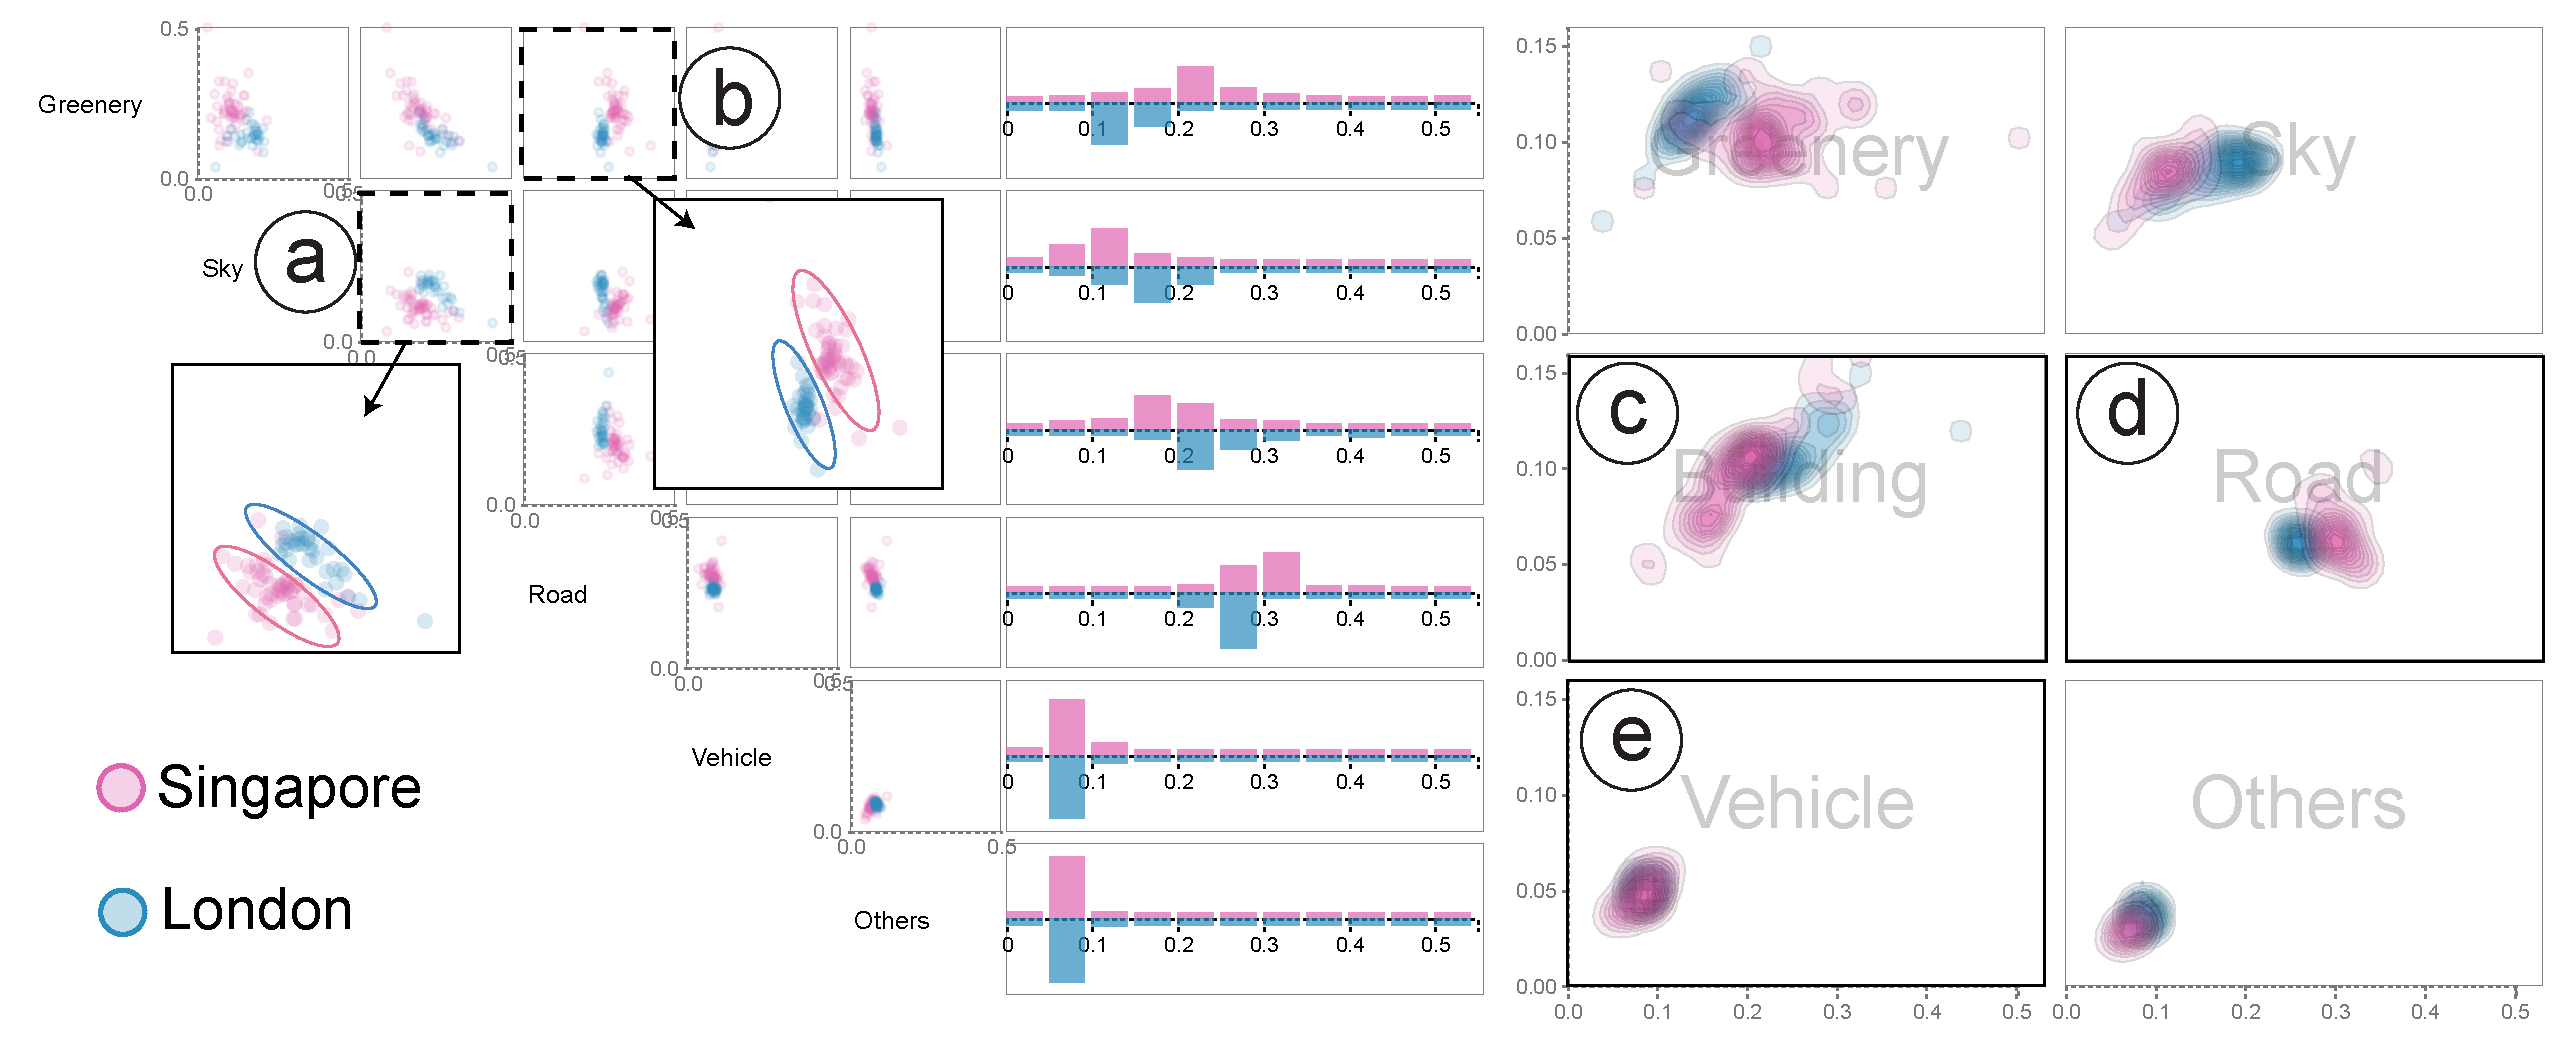
\includegraphics[width=\columnwidth]{figure/streetvizor/fig8_study_1/study_1_statistic}
	\vspace{-7mm}
	\caption{AOI Statistic View in coordination with Fig.~\ref{fig:c1_study_1_spatial} presents quantitative measurements differences of human-scale urban forms in Singapore (red) and Greater London (blue).}
	\label{fig:c1_study_1_statistic}
	\vspace{-1mm}
\end{figure}



%=================================================
\subsection{City-scale Comparison}

\textit{Comparing Spatial Distribution}.
With the AOI Map View, our system allows users to compare spatial distributions of human-scale urban forms in two AOIs (T.1.1).
Fig.~\ref{fig:c1_study_1_spatial} presents a comparison between Singapore (left) and Greater London (right).
As shown in the figure, more orange points surround the highlighted white circle, whereas more green points can be found at marginal areas in Greater London.
This indicates that more buildings are constructed around the City of London, reflecting that this city is more urbanized compared with other areas.
By contrast, Singapore's urban forms are evenly distributed.
More orange points are found in the highlighted downtown and region hubs, and more green points can be found in natural areas.
Our collaborator $SR$ explained the reason for the different spatial distributions of urban forms in Greater London and Singapore: Greater London likely expanded its urbanization from the City of London to surrounding areas, whereas Singapore, as an island city, cannot expand.
% The reason of this difference between Greater London and Singapore may be that Grater London expands its urbanization from City of London to surrounding areas, while Singapore as an island city cannot expand, as explained by our collaborator $SR$.

\vspace*{2mm}
\noindent
\textit{Comparing Quantitative Measurements}.
We can further explore the differences in quantitative measurements with AOI Statistic View (T.2.1 \& T.3.3).
Fig.~\ref{fig:c1_study_1_statistic} shows the AOI Statistic View in coordination with Fig.~\ref{fig:c1_study_1_spatial}.
From the scatterplot matrix, we find that $greenery$ and $building$ features are negatively correlated.
This result is the same as that shown in Fig.~\ref{fig:c1_statistic_view}(d).
Given that $buildings$ are artifacts and $greenery$ is natural, the negative correlation between $building$ and $greenery$ features in all four cities indicates that artifacts increase and natural environments decrease with increasing urbanization.
To improve livability, many urban planners have proposed integrating more natural spaces in street space.
In addition, Fig.~\ref{fig:c1_study_1_statistic}(a) shows that $sky$ and $building$ ratios are higher in London than in Singapore.
By contrast, $greenery$ and $road$ ratios are higher in Singapore than in London (Fig.~\ref{fig:c1_study_1_statistic}(b)).
These findings can also be found from the middle histogram bar charts.
In addition, the diversity views further show some interesting patterns.
For example, $building$ and $road$ diversities are more concentrated in London than those in Singapore, as shown in Fig.~\ref{fig:c1_study_1_statistic}(c) \& (d), and likely resulted from the different standards for building and road construction in the two cities.
$Vehicle$ usage rates are low in both cities, as shown in Fig.~\ref{fig:c1_study_1_statistic}(e).


%=================================================
\subsection{Region-scale Exploration}
\begin{figure}[t]
	\centering
	\includegraphics[width=0.98\columnwidth]{figure/streetvizor/fig9_study_2/region-functionality.png}
	\vspace{-5mm}
	\caption{Top three districts with highest $building$ ratios, while bottom three with highest $greenery$ ratios in Hong Kong.}
	\label{fig:s1_region-funcitonality}
	\vspace{-4mm}
\end{figure}
Given that human-scale urban forms are highly associated with the daily lives of residents, we posit that urban forms could reflect the functionalities of a region.
Study 1 already reveals the negative correlations between $greenery$ and $building$ features, and we hypothesize that these two urban forms can reflect urbanization levels.
To evaluate the hypothesis, we further explore these two features at region-scale (T.1.1).
Using ranking functions, we sort administrative districts in Hong Kong based on these two features.
Fig.~\ref{fig:s1_region-funcitonality} presents an overview of three districts with highest values for each feature.
The top three districts are Yau Tsim Mong, Wan Chai, and Kowloon City.
They are all business centers in Hong Kong, and we find these districts are mostly covered by orange points ($building$). 
By contrast, the bottom three districts contain highest values for $greenery$.
In particular, the greenest district is Southern Island, which is reserved as country parks.
The other two districts are also well-known natural areas in Hong Kong.
 
\begin{figure}[t]
	\centering
	\includegraphics[width=\columnwidth]{figure/streetvizor/fig9_study_2/study_2_2}
	\vspace{-7mm}
	\caption{Region-scale comparison of Tanglin in Singapore with Central Park in New York City.}
	\label{fig:c1_center-park-tanglin}
	\vspace{-1mm}
\end{figure}

In addition to exploring regions with different functionalities, urban planners are also interested in comparing regions with similar functionalities.
Here, we leverage our knowledge of famous regions in two different cities, i.e., Tanglin in Singapore (see the region highlighted as natural in Fig.~\ref{fig:c1_study_1_spatial}) and Central Park in New York City.
Both of these regions are well-known parks.
After selecting these regions, we find that nearly all streets in the two regions are dominated by green points, indicating that both regions contain considerable $greenery$ as intended.
However, we find some differences between these two regions by looking deeper into the Street Statistics View (Fig.~\ref{fig:c1_center-park-tanglin}).
First, through the feature histogram bar charts, we find that Central Park has slightly higher $greenery$ ratios (A1), whereas Tanglin has slightly higher $building$ ratios (A2).
Though these differences are marginal, they reflect that more buildings are present in Tanglin, partially because Singapore tries to maximize land usage for building construction.
In addition, by grouping street views based on street units, we glean more information from the diversity plots.
Here, we first obtain the overview that $greenery$ feature has relatively higher mean values and deviations than the other five features.
We also find some anomalies.
For example, some streets have relatively low mean values but high deviations for $greenery$ in Central Park (B1), whereas certain streets have high sky visibility in Tanglin (B2), and some streets have very high $building$ ratios in both regions (B3).

The results of this study show that human-scale urban forms are correlated with regional functionalities.
Meanwhile, even though two regions may have the same functionalities, street spaces in regions can be different between two cities.
This may reflect the differences in city planning and development strategies between cities.


%=================================================
\subsection{Street-scale Comparison}
Our collaborating domain expert $SR$ is interested in comparing the fine-grained details of two streets (T.1.2).
StreetVizor meets this requirement with Street Explorer.
Here, we select one street from Brooklyn, New York City, and one from Kowloon, Hong Kong.
Both streets are representative streets of each district.

Fig.~\ref{fig:c1_study_3} presents the visual comparison of these two streets.
The map views provide an overview that nearly half of the street views are mostly green ($greenery$), and the other half are mostly orange ($building$) on the street from Brooklyn.
By contrast, the street views in Kowloon are mostly orange ($building$).
We can observe more details by looking at the street view images.
As shown on the top images, more $greenery$ and $sky$ with low $buildings$ are seen in the left two images, whereas the right two images are filled with $building$ and $road$.
The tree map of the leftmost image shows the street view is well balanced with $greenery$, $road$, $building$, and $vehicle$ features.
Notice that the street view is also highlighted in the bottom Street Statistic View.
More details on the quantitative measurements of street views can be observed in the bottom Street Statistic View.
The themeriver plots clearly show differences in feature distributions:
street views in Brooklyn are more mixed with balanced $greenery$, $sky$, $building$, $road$, and $vehicle$ features, whereas street views in Kowloon are mostly filled with $building$ and $road$ features.
The histogram bars in PCP further confirm this observation: most street views in Kowloon have less than 10\% $greenery$ and $sky$.

Though it is well known in the field of urban planning that New York City is well integrated with natural features and that Hong Kong has more high-rise buildings, $SR$ is excited to see our system can present these differences so intuitively.
``Street Explorer can definitely improve our work efficiency,'' $SR$ commented.


\begin{figure}[t]
	\centering
	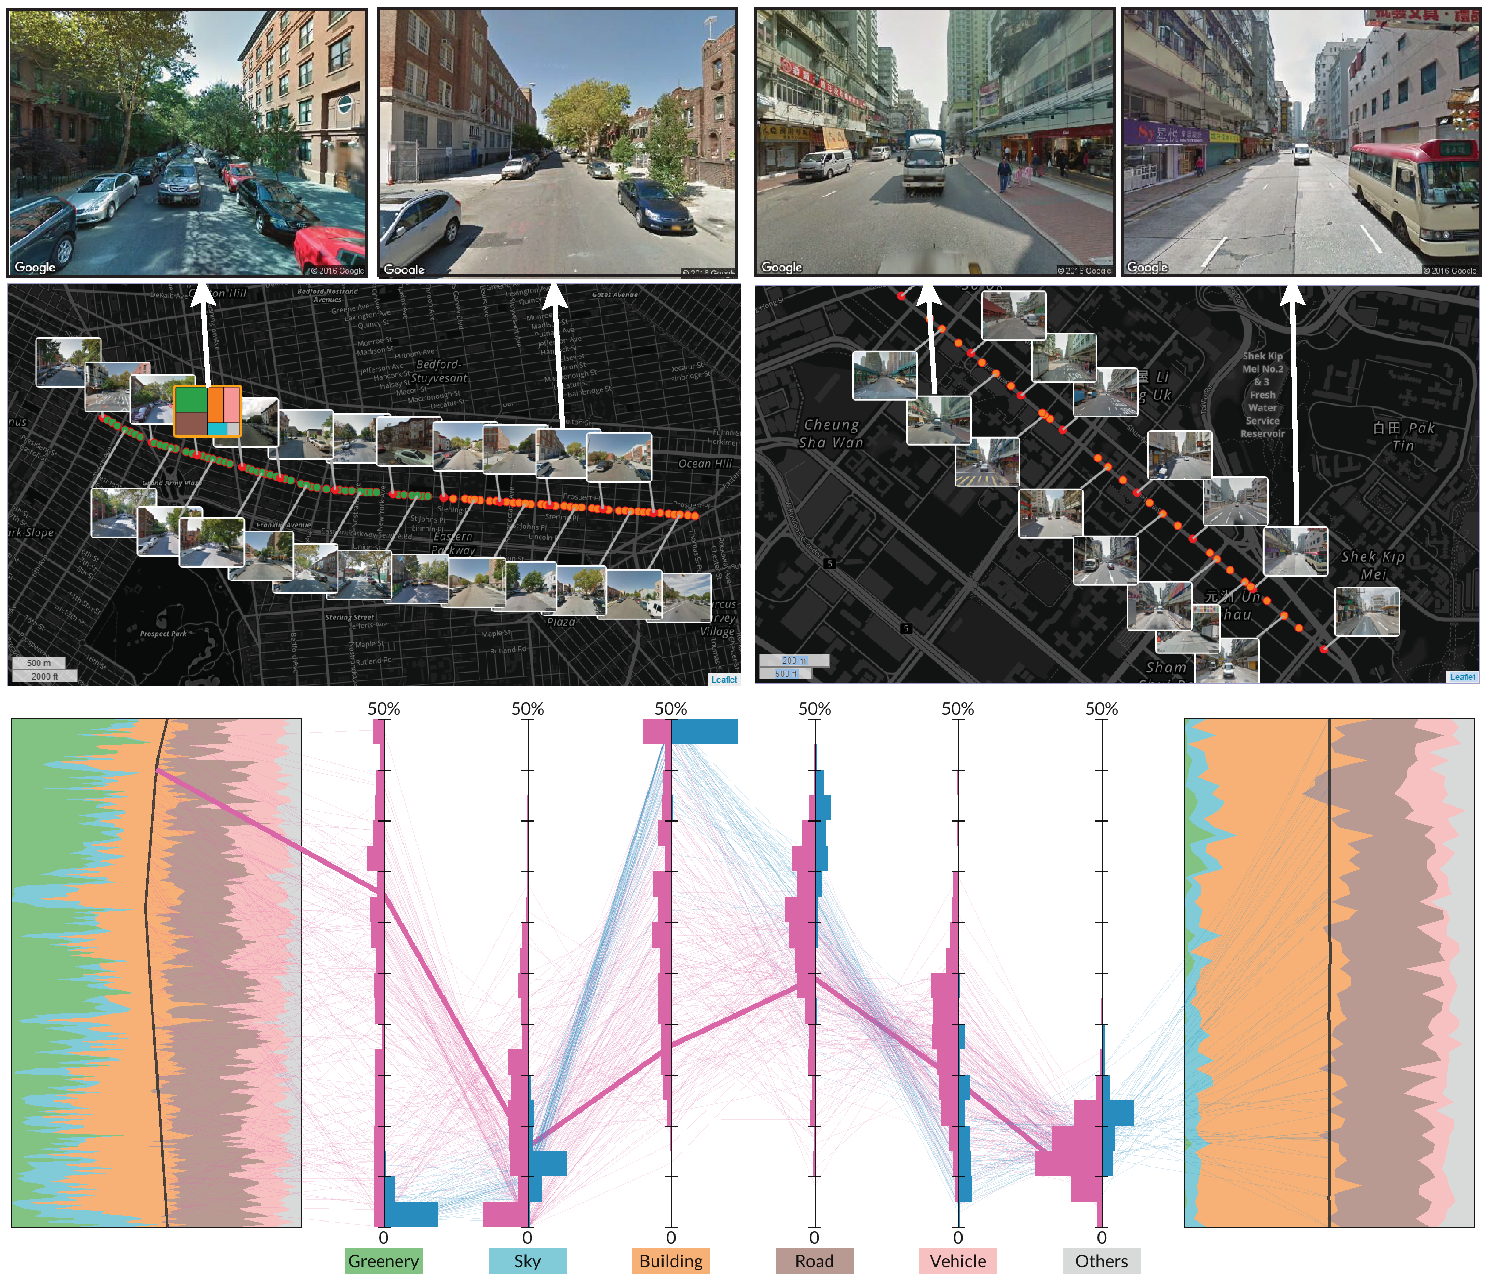
\includegraphics[width=0.95\columnwidth]{figure/streetvizor/fig10_study_3/study_3}
	\vspace{-4mm}
	\caption{Street Explorer compares the differences in human-scale urban forms of two streets in Brooklyn, New York City (left) and Kowloon, Hong Kong (right).
	The left street views contain more balanced features, whereas the right street views are dominated by $building$ and $road$.}
	\label{fig:c1_study_3}
	\vspace{-1mm}
\end{figure}
\section{Expert Review}

To evaluate the effectiveness of StreetVizor, we conducted expert interviews with two independent domain experts other than our collaborating senior researcher $SR$.
One of them focuses on designing livable public space (denoted as $EA$), and the other is an urban ecologist aiming at improving greenery in cities (denoted as $EB$).
Hence, the experts are from different backgrounds: $SR$ and $EA$ in urban planning, while $EB$ in ecology.
In the interviews, we started with explaining the visual encodings and interface design, and demonstrated to them how our system works.
Then, we showed them the case studies, and allowed them to explore the system by themselves for about twenty minutes in the end.
In general, both experts agrees that the way we study human-scale urban forms with street view images is a promising direction.
Their detailed feedbacks are summarized below.

\vspace*{2mm}
\noindent
\textit{Methodology and Approach}.
$EA$ agreed with $SR$ that evidence-based urban design is becoming a trend in urban planning.
He commented, ``StreetVizor is far more than simply a visualization platform. 
Rather, it is an excellent combination of machine learning and visualization techniques, together with classical urban design theories in place-making''.
$EB$ also expressed that ``street view images as an emerging data source can reflect urban environments well", and a visual analytics system can greatly facilitate the exploration of street views.

\vspace*{2mm}
\noindent
\textit{Interactive Visual Design}.
Both experts confirmed that StreetVizor is nicely designed according to the problem domain.
They appreciated the visual consistency across different views.
$EA$ highlighted ``it is very important to use the same colors in different views". 
$SR$ agreed the workflow of ranking multiple AOIs/streets with Ranking Explorer, and comparing two AOIs/streets for details through AOI and Street Explorer is helpful.
``It is easier for me to identify interested regions, such as those in Hong Kong (Fig.~\ref{fig:region-funcitonality})", commented by $SR$.
% They agreed the workflow of over-viewing human-scale urban forms at city- and region-scale first, and examining details at street-scale is helpful.
The AOI Explorer is nicely designed with intuitive map and statistic views.
In particular, ``the statistic view seamlessly integrates three easily understandable plots'', commented by $EB$.
By referring to the scatterplot matrix in Fig.~\ref{fig:statistic_view} \& Fig.~\ref{fig:study_1_statistic}, $EA$ was excited to see the negative correlation between $greenery$ and $building$ $-$ ``there are much space to improve".
$EA$ also liked the visual comparison of human-scale urban form distributions over space (Fig.~\ref{fig:study_1_spatial}), as it reflects the differences of urbanization process and master plans in different cities.

The experts thought presenting street view images in the Street Explorer is intuitive, and mouse hover over to show tree map is helpful.
In contrary, it was difficult in the beginning for both experts to understand the PCP enhanced with street layout information, especially the themeriver plot.
But after exploration, they agreed it is an excellent idea, as it clearly reveals the feature distributions along street.
``Though not common, I believe there are many applications and potentials for the enhanced PCP'', commented by $EB$. 

\vspace*{2mm}
\noindent
\textit{Applicability}.
Both domain experts would like to apply our system to deal with practical problems in their domains. 
Expertized in urban planning and design, $EA$ emphasized ``the lack of efficient tools for human-scale management and design obstacles creating high-quality urban streets.''
 StreetVizor has a great potential to be employed by planners and designers to ``build more pedestrian-oriented and livable streets.'' 
$EA$ also commented ``StreetVizor is highly applicable for evaluating case studies in urban planning''. 
For example, planners can select several key areas, e.g., CBDs, among different cities and then compare their spatial features to develop appropriate strategies in urban renewal.
$EB$ would like to apply our system in environment monitoring, since ``the large amount of GSV images can provide rich information of urban environment''.
He suggested to extend our system in exploring a time-series street view dataset, so that it would allow him to monitor environment changes.

\vspace*{2mm}
\noindent
\textit{Limitations and Improvements}.
The experts pointed out some limitations in our system.
In this work, we explore only six features of human-scale urban forms.
Both experts suggested to extract more urban forms, such as aesthetic amenities and mental well-being, from street view images.
This will advance our system's analytical capabilities and extend its applicabilities.
For instance, a recent study~\cite{jiang_2014_dose} shows that certain relationship may exist between street greenery \& sky ratio and the risk of health challenges.
Besides, they proposed to improve our visual designs.
$EB$ noticed the feature histogram bars in AOI and Street Statistic View are designed differently: one in horizontal, and the other one in vertical style.
He felt the vertical histogram bars are confusing, as they ``do not fit our work habits''.
$EA$ suggested the Street Statistic View can be further improved, by ``encoding neighboring street layouts in the plot'', to reflect spatial information better.

\section{Discussion}
\label{sec:c1_discussion}

In this work, we combine automatic machine learning and interactive visual analytics techniques to explore human-scale urban forms.
The combination of methods tackles the challenges of integrating information from multiple perspectives and at different scales for analysis.
This approach is attractive for urban planners~\cite{liu_2015_understanding, long_2017_how} because it shows the possibility of transferring traditional subjective and intuitive-oriented urban design to evidence-based and big-data informed methods.
%The case studies show that our approach effectively assist domain experts in finding the street view patterns of interest.

The analysis of human-scale urban form in this work relies heavily on a deep learning technique for image classification.
Therefore, classification accuracy poses serious challenges in our approach.
We select SegNet, which achieves a global accuracy of 82.8\%, out of the different classification techniques that we tried.
The case studies show that the classification technique could provide reasonable analytical results on city- and region-scale human-scale urban form patterns.
Nonetheless, the results remain unsatisfactory in many cases, especially when users would like to examine fine detailed urban forms at street-scale.
We envision applying a more advanced classification algorithm in the near future, given the rapid evolution of image classification techniques.
In addition, the classification is preprocessed offline.
Our system does not support the analysis of street views queried on runtime. 
Thus, its applicability is limited and domain knowledge of planners are underutilized in exploring street views in other cities.
This deficiency can also be resolved with advancement in image classification algorithms and machine computing capabilities.

Moreover, we expect that our system will face scalability issues when the number of street view images increase (e.g. when analyzing street views in more cities). 
To tackle this problem, we can integrate more advanced data structures, such as nanocubes~\cite{lins_2013_nanocubes} or Gaussian cubes~\cite{wang_2017_gaussian} for spatial data querying.
More levels of detail and abstraction can also be introduced to handle this problem.
The increase in image number will also burden street view clustering in the interactive exploration process.
We anticipate that certain pre-configurations will facilitate this process.

Presenting multivariate data with spatial information is challenging.
We tackle this challenge by integrating popular PCP with a themeriver plot along an adjusted street layout.
The case studies and feedbacks from experts demonstrate the effectiveness of this design.
Nonetheless, there are some issues with our design.
First, it represents street layout as a simple spline, which is not sufficiently intuitive when the street is straight.
We plan to encode more semantic labels, such as neighboring streets, in the design, as suggested by $EA$.
Second, although the majority of the streets (over 95\%) that we have explored can be rotated and fitted in the rendering space, adjustment does not work in some cases.
Typical examples are streets in a spiral layout.
A more general approach should be developed that can reveal the street layout intuitively and seamlessly fit the street layout in the rendering space.

\input{chapter/2_StreetVizor/10_Conclusion}

% \chapter{Route-Aware Edge Bundling for Visualizing Origin-Destination Trails in Urban Traffic}\label{chap:c2_intro}

Origin-destination(OD) trails describe movements across geographical locations, which can be visualized as direct lines connecting ODs.
The visualization method, however, causes clutter issues for large amounts of OD trails.
Edge bundling methods can mitigate the problem, yet bundling OD trails in urban traffic data remains under-explored.
This work presents a new approach, namely route aware edge bundling (RAEB), specifically designed to fill the gap.
We identify inconsiderate settings of conventional kernel density estimation edge bundling (KDEEB) when applied to urban traffic data, including non-optimal kernel size and road neglect.
The limitations are addressed in RAEB by introduction of a comprehensive pipeline comprising preprocessing, bundling and evaluation processes.
A series of new parameters, together with adaptions of existing ones, are employed in the pipeline.
Experiments with artificial and real-world traffic data demonstrate advancements of RAEB in various applications, including preservation of road network topology and support of multi-scale exploration.


\section{Introduction}
\label{sec:intro}

Movement can be defined as change of an object's positions or geometric attributes over time~\cite{dodge_2008_towards}.
Within a specific time period, the movement of an object can be modeled with an origin (O), a destination (D), and consecutive positions (trail) in-between.
Due to fast development of location sensing technologies, massive amounts of OD trails, such as vessel movements and taxi trips, have been collected.
Studies of OD trails have revealed many movement patterns and contributed to many applications, e.g. diseases spread control~\cite{brock_2006_scaling} and transportation planning~\cite{wang2012understanding}.

Visualizing OD trails is a hot yet challenging topic.
Conventional method that connects origins to destinations with lines~\cite{tobler_1987_experiments} can easily cause visual clutter.
To tackle the problem, methods of aggregating trails into flows are usually employed.
A number of automatic techniques have emerged, such as intelligent routing layout~\cite{phan2005flow, verbeek_2011_flow} and spatial mapping~\cite{andrienko_spatial_2011-1, guo2014origin}.
These methods are preferable for revealing overall traffic patterns for answering general questions, e.g., what are popular roads in a city? where do people head to?
However, the methods mostly ignores information of individual OD trail.
In certain scenarios such as to find abnormal people movements, additional analytics are required to complement the visualization.

Wrapping up OD trails into bundles can reveal overall traffic patterns, meanwhile keep individual OD trail.
Many bundling methods including spring-based (e.g.,~\cite{holten2009force, selassie2011divided}), image-based (e.g.,~\cite{hurter2012graph, lhuillier2017ffteb}), and geometry-based (e.g.,~\cite{holten2006hierarchical, cui2008geometry}), have been proposed.
These techniques have been successfully employed for many different datasets such as Internet connections and migrations.
In these data, it is flexible to manipulate edges as long as node connections are kept.
This, however, does not hold for OD trails in urban traffic data.
In a city, humans and vehicles are moving along roads, and many activities including traffic jams and accidents, are happening on roads.
Hence, OD trails are constrained by road networks.
Trail information is equally, if not more, important as ODs for urban traffic data.

Among various edge bundling methods, kernel density estimation (KDEEB)~\cite{hurter2012graph} is in state-of-the-art with advantages in speed and generality.
However, we identify several inconsiderate settings of KDEEB when applied to OD trails in urban traffic data, including non-optimal kernel size and road neglect.
These settings wreck applicability of KDEEB for movement visualization, which requires to preserve road network topology and to support multi-scale exploration.
This work presents a new method, namely route-aware edge bundling (RAEB), specifically designed to address the limitations.
RAEB employs a comprehensive pipeline consisting of preprocessing, bundling and evaluation processes.
A series of new parameters such as route awareness and bundling stability, which leverage advanced techniques from geography and image processing fields, are introduced.
Experiments on artificial and real-world urban traffic data show that RAEB can generate more realistic results, meanwhile achieve fast computation speed comparable to KDEEB.

\vspace{1.5mm}
The primary contributions of this work include:

\begin{itemize}

\item
We develop a new edge bundling method of RAEB, which includes a comprehensive pipeline consisting of preprocessing, bundling, and evaluation processes. 

\item
We adapt existing parameters in KDEEB, and introduce a series of new parameters, to better fit OD trails in urban traffic.

\item
We conduct several experiments using artificial and real-world urban traffic data to demonstrate effectiveness of RAEB. 
\end{itemize}
% \vspace*{-1mm}
\section{Related Work}
\label{sec:related_work}

This section discusses previous studies closely related to our work.

%===============================================
\subsection{Street View Analysis}
GSV system provides high quality and accurate panoramic images of hundreds of cities~\cite{anguelov2010google}.
In recent years, researchers studying human-scale urban forms have utilized GSV images as a new and convenient data source. 
For example, researches have shown that the analysis of GSV images can be used to audit neighborhood environments~\cite{rundle_2011_using}, quantify street greenery~\cite{li_2015_accessing}, and predict street safety~\cite{Naik_2014_streetscore}.
Nonetheless, the majority of these studies face scalability issues given their focus on either a particular feature~\cite{li_2015_accessing} or a small area~\cite{rundle_2011_using, Naik_2014_streetscore, li_2015_accessing}.
Thees issues can be addressed by incorporating deep learning techniques, which can be used to summarize city landscapes~\cite{doersch2015makes} and estimate the demographic makeup of a country~\cite{gebru2017using}.

In this work, we collect $\sim$1.7 million GSV images of four representative mega-cities, and apply a deep learning technique~\cite{Badrinarayanan_2015_segnet} to automatically extract desired urban forms from the collected images.
More importantly, we develop an effective visual analytics tool for urban planners to explore human-scale urban forms.

%===============================================
\subsection{Urban Data Visualization}
Vast amounts of urban data, including traffic~\cite{ferreira_visual_2013, wang_2013_visual}, social media~\cite{xu_2013_visual, chen_2015_interactive}, environment~\cite{ferreira_2011_birdvis}, and simulated urban spaces~\cite{vanegas_2009_visualization}, have been collected in an urban context.
Big urban data brings in unprecedented opportunities for evidence-based urban design, and visualization systems can assist domain experts in finding evidence from the data.
A systematic overview of visualization systems can be found in~\cite{zheng_2016_visual}.

Qu et al.~\cite{qu_2007_visual} presented a comprehensive visualization system for the analysis of a city's air pollution that affects the daily lives of residents.
Their system integrates parallel coordinates and scatterplots to show relationships between high-dimensional air pollutants.
In addition to air pollution, landmark visibility is related to the daily experience of a city's residents.
Ortner et al.~\cite{ortner_2016_vis-a-ware} visually compared the effects of candidate buildings on landmark visibility from various viewpoints.
In this system, users can select a series of ranking schemes, and candidate buildings are then automatically sorted.
Similar to our present work, Arietta et al.~\cite{arietta_2014_city} associated visual elements with city attributes, including violent crime rates and housing prices.
They developed various prototype visualizations, such as the visual boundary of urban neighborhoods.

% \vspace{2mm}
Although different data are explored, these visualizations similarly employ CMVs, because urban data typically exhibits both spatial information and multi-dimensional attributes.
Our system also adopts this empirical approach.
In addition, to address specific domain problems, we develop effective visualization techniques, including a novel parallel coordinates enhanced with street layouts.

%===============================================
\subsection{Multivariate Geographical Data Visualization}
Visualizing multivariate data is a hot topic in the visualization field.
Numerous conventional approaches to this topic have been developed, and can be classified into two groups:
1) employing visualization techniques, such as parallel coordinates plot (PCP), scatterplot matrix, and start coordinates;
and 2) projecting data points onto a two- or three-dimensional visual space that can be directly plotted on a screen, such as multidimensional scaling and principal component analysis.
All these approaches have pros and cons.
For example, although PCP presents all dimensional attributes without information loss, it can easily generate visual clutter with big data and pairwise correlations can only be shown on two nearby coordinates~\cite{heinrich_2012_state}.
Many improvements have been developed to address these issues.
These improvements include edge bundling to reduce visual clutter~\cite{zhou2008visual, holten_2010_evaluation}, and hierarchical data clustering and the navigation of resulting structures~\cite{fua1999hierarchical, zhao_2012_structure}.
% ., and sort dimensions in order based on their correlations~\cite{zhao_2012_structure, wu_2015_telcovis}.

When multivariate data is dependent upon locations, the analytical tasks become more complex because geographical information needs to be revealed.
Turkay et al. developed \textit{Attribute Signature}~\cite{turkay_2014_attribute}, which employs a geographical map and small multiples of multivariate attributes to show geographic variability in attribute statistics.
Goodwin et al.~\cite{goodwin_2016_visualizing} further explored multivariate geographical data across scales by adopting new designs to show correlation, scale, and geographical information.
The frameworks proposed by both studies can be generalized to explore multivariate geographical data.

In this work, human-scale urban forms to be explored are also multivariate geographical data: the features are in six dimensions and they are dependent on locations.
We leverage the advantages of scatterplot matrix and PCP for different analytical tasks.
Specifically, we employ scatterplot matrix for exploring features at city- and region scales given that it can effectively reveal correlations between all pair-wise features.
We also arrange the views in a way similar to \textit{Attribute Signature}~\cite{turkay_2014_attribute}, i.e., geographical information is presented on maps and multivariate attributes in small multiples. 
In addition, we develop a novel PCP enhanced with a themeriver plot, which fits better with the analytical task of showing feature variations along street layout at street-scale.

%===============================================
\subsection{Comparative Visualization}
Gleicher et al.~\cite{gleicher_2011_visual} classified techniques for visual comparison into three categories:
1) Juxtaposition, i.e., presenting objects next to each other. 
For example, NodeTrix~\cite{yang_2017_blockwise} arranges two human brain networks side-by-side. 
2) Superposition, i.e., presenting multiple objects on top of one another.
Typical examples are time-series line graphs that plot the changes in several variables over time in the same coordinate system.
3) Explicit encoding, i.e., presenting differences or correlations between objects visually.
For instance, the bivariate density map is employed in~\cite{zeng_2017_visualizing} to show the relationship between departure and arrival movements over space.
In practice, these techniques are combined to address complex analytical tasks.

Our work adopts juxtaposition that arranges maps of two AOIs/streets side-by-side (Fig.~\ref{fig:teaser}(b) \& (d)), and superposition to compare multivariate features of two AOIs/streets in the same coordinate system (Fig.~\ref{fig:teaser}(c) \& (e)).

\if 0
\subsection{Human-scale Urban Form}
Though human-scale urban form is defined recently~\cite{long_2016_human-scale}, discussions of the concept in urban planning and designing have a long history that can be traced to 1960s.
A series of pioneering studies~\cite{jacobs_1961_life, gehl_1971_life} claimed the positive effects of human-scale urban form in designing high-quality urban space.
Among various types of human-scale urban form, the visible one is particularly important as human beings tend to pay most attentions to surroundings that can be directly seen~\cite{gehl_1971_life}. 

Accompanying with the raising of big open data, e.g., GSV images, researches in studying visible human-scale urban form are focusing on quantitatively measuring the related features nowadays. 
For example, researches have shown that analyzing GSV images can audit neighborhood environments~\cite{rundle_2011_using}, quantify street greenery~\cite{li_2015_accessing} and predict street safety~\cite{Naik_2014_streetscore}.
Nonetheless, most of these researches got scalability issues as they focused on either a particular feature or a small area.
The issues can be addressed by incorporating deep learning techniques, by which recent studies have shown its applicability in summarizing landscape of a city~\cite{doersch2015makes} and even estimating demographic makeup of a country~\cite{gebru2017using}.

\vspace{2mm}
In this work, we first identify the important features of visible human-scale urban form, then collect millions of GSV images across four representative mega-cities, and apply a deep learning technique - SegNet~\cite{Badrinarayanan_2015_segnet} - to automatically label related features in the images.
More importantly, we develop an effective visual analytical tool for urban planners to explore the analysis on demand.

\fi

\if 0
\subsection{Street view images analysis}

Google street view(GSV) is a well know system that provides panoramic images in hundreds of cities of more than 20 countries to millions of googles users. During the past 15 year, GSV system can provide a good quality and accurate images service, and more and more researchers begin to focus on this data source\cite{anguelov2010google}. GSV is considered as a novel and convenient way to collect environmental information and has been utilized in a broad range of research domains including ecology, geography, archeology, urbanology and even some social science. 

In recent years, the researchers in the ecology field found that the GSV images was an alternative way to observe the natural environment. Olea et al. \cite{olea2013assessing} discussed that the GSV images could be a good data source to assess the habit of some cliff living animals and the using of both of these two methods could be highly useful as a coarse-scale assessment method over large geographic areas. Hardion et al.\cite{hardion2016species} proposed a  time and cost-effective solution using the geo-located street view images in the analysis of species distributions. In the discipline of urbanology and sociology, GSV has been used in the virtual audit of different physical environment\cite{clarke2010using, rundle2011using, kelly2013using, vanwolleghem2014assessing} in the city. These methods has the potential to significantly reduce the costs and time of collecting data and can be well adapted in the large geo-scale research. 

Even though the GSV images could be adapted in different research areas, in the most instance, the observation of environment is still conducted by human beings. Nowadays, fast developed of deep learning techniques has been widely used in image processing, many research has considered the automatic methods to further reduce the human cost. Doersch et al.\cite{doersch2015makes} analyzed millions of image from GSV to extract the visual features commonly occurred to summary the landscape of a city. Timnit et al.\cite{gebru2017using} also proposed a method use deep learning techniques and GSV images to estimate teh demographic makeup of United States.
\fi

\section{Problem Statement and System Overview}
\label{sec:overview}

This section briefly describes KDEEB algorithm, followed by a discussion of inconsiderate settings when applied to OD trails in urban traffic.
An overview of RAEB is presented at the end.

\begin{figure}[t] 
	\centering
	\includegraphics[width=0.495\textwidth]{fig2_kernel_size/kernel_size}
	\vspace{-5mm}
	\caption{KDEEB applied to taxi trips in Manhattan with different kernel sizes $p_r$: (a) 120, (b) 80, (c) 40, and (d) 20.
	More detailed bundles are generated with smaller $p_r$.}
	\label{fig:kernel_size}
	\vspace{-5mm}
\end{figure}

%%%%%%%%%%%%%%%%%%%%%%%%%%%%%%%%%%%%%%%%%%%%%%%%%%%%%%%%%%%%%%%%%%%%
%%%%%%%%%%%%%%%%%%%%%%%%%%%%%%%%%%%%%%%%%%%%%%%%%%%%%%%%%%%%%%%%%%%%

\subsection{KDEEB Algorithm}
\label{ssec:kdeeb}
KDEEB is a fast edge bundling method for visualizing dense graphs.
It employs a general pipeline with edge sampling, splatting, gradient estimation, edge advection, and bundle smoothing.
In edge sampling step, an edge $\textbf{e}_i$ is divided into uniformly-sampled polylines, i.e., $\textbf{e}_i = \{\textbf{x}_j\}$, with user-given sampling step $\sigma$.
After that, KDEEB computes a density map $\rho : \mathbb{R}^2 \rightarrow \mathbb{R}^+ $as

\vspace{-4mm}
\begin{equation}\label{eq:kernel_density_estimation}
\rho(\textbf{x} \in \mathbb{R}^2) = \sum_{\textbf{y} \in D} K (\frac{\|\textbf{x}-\textbf{y}\|}{p_r})
\end{equation}

where $K$ is a parabolic radial kernel and $p_r$ is kernel radius.
Next, each edge sampling site $\textbf{x}_j$ is advected to a new position $\textbf{x}'_j$ as:

\vspace{-5mm}
\begin{equation}\label{eq:advecting_points}
\textbf{x}'_j = \textbf{x}_j + p_r \frac{\nabla \rho}{||\nabla \rho||}
\end{equation}

Finally, a smoothing function is applied on $\textbf{x}_j$ to remove jitters created by the advection step.
These steps are repeated $p_n$ times until stable bundles are generated.

\vspace{2mm}
\noindent
\textit{Parameter Setting}.
KDEEB requires several parameters to be preset by users.
Following settings are recommended~\cite{van2016cubu}:
\begin{itemize}

\item 
Kernel radius $p_r$: Initial value set to 5\% of graph drawing size.
A constant decay ratio $\lambda$ in [0.5, 0.9] is applied to $p_r$ at each bundling iteration $n$.

\item
Bundling iteration $p_n$: An integer in between 10 to 15.

\end{itemize}

\begin{figure*}[t]
	\centering
	\includegraphics[width=0.995\textwidth]{fig3_framework/framework2.pdf}
	\vspace{-3mm}
	\caption{Overview of RAEB pipeline.
	Our method mainly consists of three phases: \textit{Preprocessing} for creating a proper initial layout, \textit{Bundling} for bundling input OD trails, and \textit{Evaluation} for generating a stable bundle structure.}
	\label{fig:framework}
	\vspace{-4mm}
\end{figure*}

%%%%%%%%%%%%%%%%%%%%%%%%%%%%%%%%%%%%%%%%%%%%%%%%%%%%%%%%%%%%%%%%%%%%
\subsection{Problem Identification}
The parameter settings are recommended for general graphs that consist of fixed nodes and connections between them.
For such a graph, it is free to manipulate node connections into smooth polylines.
However, when applied to OD trails in urban traffic data, KDEEB encounters the following issues.

\begin{itemize}
\item
\textit{P1: Non-optimal Kernel Radius}.
Kernel radius $p_r$ in KDEEB is solely based on graph drawing size, while ignores geometric properties of road network.
Figure~\ref{fig:kernel_size} presents KDEEB results generated with different kernel sizes for taxi trips in Manhattan: 120, 80, 40, and 20 in (a) - (d), respectively.
Sizes for graph drawing are all 720$\times$1440, thus KDEEB would recommend $p_r$ = 80 as 5\% of graph graphing size.
However, smaller $p_r$ generate more detailed and visual appealing bundles, comparing Figure~\ref{fig:kernel_size}(b) to (c) \& (d).
This happens because most space in graph drawing are not utilized, due to the long and thin shape of Manhattan island.
In addition, urban traffic can unevenly spread in a city, such as Shenzhen taxi data (Section~\ref{ssec:study3}), making small $p_r$ preferable.

\vspace{1mm}
\item
\textit{P2: Road Neglect}.
Urban traffic are moving along roads in a city, thus OD trails should be constrained to roads in a city.
However, KDEEB represents each OD connection with a direct line, while ignores information about the road network.
Thus, resulting bundles can be displaced far away from the roads.
This can cause impression of traffic moving in wrong positions, such as those bundles in between Manhattan and Brooklyn (Section~\ref{ssec:study1}).
The displacements can also add difficulty to mentally map original OD trails with resulting bundle lines.
\end{itemize}

\vspace{2mm}
\noindent
Besides, KDEEB lacks a quantitative method to automatically terminate bundling iterations.

\begin{itemize}
\item
\textit{P3: Preset Bundling Iterations}.
KDEEB is an image-based edge bundling method. 
Most of these bundling methods generate bundling results in an iterative way. 
The number of bundling iterations $p_n$ is preset based on practical experience: 10 in KDEEB~\cite{hurter2012graph}, while 15 in CUBu~\cite{van2016cubu}.
The numbers are chosen because tight and stable bundles are generated.
However, these conditions are rather subjective, which can vary among individuals and may be affected by other parameters like image size and sampling step.
\end{itemize}

%%%%%%%%%%%%%%%%%%%%%%%%%%%%%%%%%%%%%%%%%%%%%%%%%%%%%%%%%%%%%%%%%%%%
\subsection{RAEB Overview}
We develop route-aware edge bundling (RAEB), a comprehensive edge bundling method specifically designed for visualizing OD trails in urban traffic.
As illustrated in Figure~\ref{fig:framework}, RAEB pipeline mainly consists of three parts: \textit{Preprocessing}, \textit{Bundling}, and \textit{Evaluation}.

In \textit{Preprocessing}, RAEB first generates a simplified road network from the input one such as open street map (OSM).
Raw OD trails are mapped onto simplified road network using map matching algorithms.
Together with urban traffic information, simplified road network can be organized in a hierarchical route structure.
OD trails can be abstracted accordingly depending on a new parameter of route awareness defined by users.
A value for kernel size is also measured based on geometric property of the route structure.

The abstract OD trails are passed into \textit{Bundling} stage as input graph.
Bundling process is an image-based approach similar to KDEEB workflow.
Specifically, we discard the preset parameter of bundling iteration $p_n$ in KDEEB.
Instead, we introduce a new parameter of bundling stability, which is measured as normalized mutual information between images generated by two consecutive iterations.
The measurement is done in the \textit{Evaluation} stage.
If bundling stability reaches a threshold, we terminate the bundling iteration and export a final image.
Besides, we measure Fréchet distance between generated bundles to OD trails mapped on the road network.
The measurement complements final image with a quantitative metric that reveals quality of a bundling method.

\section{Preprocessing}
\label{sec:preprocess}
%%%%%%%%%%%%%%%%%%%%%%%%%%%%%%%%%%%%%%%%%%%%%%%%%%%%%%%%%%%%%%%%%%%%%%%%%%%%%%%%%%%%%%%%%%%%%%%%%%

This work leverages both OD trails and road network to improve edge bundling quality.
This section introduces major steps in \textit{Preprocessing} stage, including: map matching, hierarchical road structure construction, and trail abstraction.

%%%%%%%%%%%%%%%%%%%%%%%%%%%%%%%%%%%%%%%%%%%%%%%%%%%%%%%%%%%%%%%%%%%%
\subsection{Basic Traffic Concepts}
\textit{Road Network}:
A road network can be modeled as a directed graph $\bar{G} = (\bar{V}, \bar{E})$, where $\bar{V}$ is the set of nodes in $\bar{G}$ and $\bar{E}$ is the set of edges connecting nodes in $\bar{V}$.
Degree of a vertex $\bar{v}$, denoted as $deg(\bar{v})$, indicating the number of edges connected to $\bar{v}$.
By this, a vertex $\bar{v} \in \bar{V}$ can be classified as an endpoint with $deg(\bar{v})=1$, a midpoint with $deg(\bar{v})=2$, or an intersection with $deg(\bar{v})>2$.
To facilitate computation, we can simply $\bar{G}$ into a simplified graph $G = (V, R)$, where $V$ is the union of endpoints and intersections, and $R$ is a set of links connecting nodes in $V$.
Each link $r$ represents a sequence of $n$ consecutive nodes in $\bar{V}$:

\vspace{-7mm}
\begin{equation}
  \begin{aligned}
  	r &:= \bar{v}_1 \rightarrow \bar{v}_2 \rightarrow ... \rightarrow \bar{v}_n, \,\,\, \forall \bar{v}_i \in \bar{V}
  \end{aligned}
\end{equation}

\vspace{-2mm}
\noindent
where $\bar{v}_1$ and $\bar{v}_n$ are endpoints or intersections, while the other nodes are midpoints.
For the sake of clarity, we use the term \textit{route} to describe such a link.
Computation tasks, including shortest path query and map matching, are performed on the simplified graph $G$.

\vspace{1mm}
\noindent
\textit{Urban Traffic}:
Thanks to open data campaign, many urban traffic data are available nowadays.
Typically, raw urban traffic data can come in either of the following forms:

\begin{itemize}
\item
\textit{UT-1}: origin and destination locations only, such as New York taxi trips~\cite{ferreira2013visual} and Singapore public transportation rides~\cite{zeng_2015_visualizing}.
Such a raw trip $t_{raw}$ can be represented as $t_{raw} := l_o \rightarrow l_d$, where $l_o$ and $l_d$ represent origin and destination locations, respectively.

\item
\textit{UT-2}: a sequence of GPS positions, such as Stuttgart scooter fleet~\cite{kruger_trajectorylenses_2013} and Hangzhou taxi trips~\cite{wang_2014_visual-reasoning}.
Such a raw trip $t_{raw}$ can be represented as $t_{raw} := l_1 \rightarrow l_2 \rightarrow ... \rightarrow l_n$, where $l_i \subset \mathbb{R}^2$. $l_1$ and $l_n$ are origin and destination, i.e., $l_o$ and $l_d$.
\end{itemize}

Both forms of urban traffic data can be generalized as a traffic graph $G_t = (L, T)$, where $L$ is the set of locations and $T$ is the set of trips represented as sequential connections of locations.

%%%%%%%%%%%%%%%%%%%%%%%%%%%%%%%%%%%%%%%%%%%%%%%%%%%%%%%%%%%%%%%%%%%%%%%
\subsection{Map Matching}
\label{section:edge_matching}

Constraining movements over an underlying road network, i.e., mapping traffic graph $G_t := (L, T)$ to road network $G := (V, R)$, is usually a preliminary step for urban traffic analysis.
This is necessary.
First, recorded locations get errors due to imprecise GPS localization, while road network is precise and constant.
Second, $G_t$ can be much more complex than $G$:
Taking New York traffic for an example, there are over millions of taxi trips per day, resulting in millions of locations $L$, yet its simplified road network contains less than 100K routes.
Therefore, map matching can enrich effective analysis and visualization.

There are many map matching methods available, including shortest path, minimum turns, and ST-matching~\cite{lou_2009_map} for GPS traces.
These methods are preferable for different dataset.
We employ the following methods for corresponding urban traffic.

\begin{itemize}

\item
For \textit{UT-1}, i.e., $t_{raw} = l_o \rightarrow l_d$, we first find corresponding closest nodes $v_o \in V$, $v_d \in V$ for $l_o$ and $l_d$ respectively.
After that, we search for the shortest path between $v_o$ and $v_d$ in $G$.

\item
For \textit{UT-2}, i.e., $t_{raw} = l_1 \rightarrow l_2 \rightarrow ... \rightarrow l_n$, we use ST-matching algorithm, which considers not only spatial features of road network, but also temporal constraints.
The method was later visually investigated and optimized with an interactive interface~\cite{kruger_2018_visual}.
\end{itemize}

Both methods return a sequence of routes $r_1 \rightarrow r_2 \rightarrow ... \rightarrow r_n$ in $G$ for each OD trail $t_{raw}$.
We then combine the routes with origin ($l_o$) and destination ($l_d$) locations of $t_{raw}$.
Thus, both types of $t_{raw}$ are converted to the same map matching form. 

\vspace{-7mm}
\begin{equation}
  	\begin{aligned}
t_{map} := l_o \rightarrow r_1 \rightarrow r_2 \rightarrow ... \rightarrow r_n \rightarrow l_d.
 	\end{aligned}
\end{equation}
\vspace{-1mm}

Here the OD trail's origin $l_o$ and destination $l_d$ are kept.

%%%%%%%%%%%%%%%%%%%%%%%%%%%%%%%%%%%%%%%%%%%%%%%%%%%%%%%%%%%%%%%%%%%%%%%%%%%%%%%%%%%%%%%%%%%%%%%%%%
\subsection{Hierarchical Route Structure Construction}
\label{ssec:hiera_road}

\begin{table}
	\centering
	\begin{tabular}{|c|c|c|}
	\hline
	Category & Exemplary OSM Indicator & Score ($r_{hier}$)  \\ \hline
	Expressway & motorway, trunk & 1 \\ \hline
	Trunk Road & primary, motorway\_link& 0.75 \\ \hline
	Secondary Road & secondary, tertiary & 0.5 \\ \hline
	Branch Road & unclassified, residential & 0.25 \\ \hline
	\end{tabular}
	\vspace{1mm}
	\caption{Route hierarchy, OSM indicator and hierarchy score} \label{tab:sometab}
	\label{table: road_score}
\vspace{-6mm}
\end{table}

A road network is usually designed in hierarchical levels to avoid dense direct connections among regions.
This inspires us to construct a hierarchical route structure to benefit edge bundling.
Although urban roads are organized hierarchically, it does not consider OD trails.
This work makes use of the following attributes of a route $r$ in $G := (V, R)$ to construct a hierarchical route structure.

\vspace{1mm}
\noindent
\textit{Route length} ($len(r)$).
Visual appearance of each OD trail is determined by its routes on road network.
Longer a route, more it will affect the visual appearance.
Thus an important component affecting route hierarchy is route length.
Here, $len(r)$ is measured in Euclidean space and normalized over the whole road network.

\vspace{1mm}
\noindent
\textit{Road hierarchy} ($hier(r)$).
Urban roads are classified into hierarchies: freeways, arterials, collectors, and local roads.
Similar descriptions can also be found elsewhere~\cite{wang_2014_visual-reasoning}.
A higher level usually indicates faster traffic speed and less access to property.
OSM provides more detailed indicators of road hierarchy, e.g., trunk, primary, tertiary, etc.
To keep consistent, we classify these indicators into four hierarchies.
A route $r$ in each hierarchy is assigned an score according to Table~\ref{table: road_score}. 

\vspace{1mm}
\noindent
\textit{Flow magnitude} ($flow(r)$).
Flow magnitude measures how many OD trails pass through a route $r$.
The previous two factors purely rely on road network, while $flow(r)$ reflects the importance of a route in consideration of OD trails.
Here, $flow(r)$ is measured by counting how many mapped OD trails passing through $r$, and then normalized. 

\vspace{2mm}
By this, each route can be represented by a vector $V(r) := <len(r), hier(r), flow(r)>$.
Score of a route $score(r)$ can be measured as $score(r) = \sum w_i \times V(r)_i$, where the weights $w_i (i = 1, 2, 3)$ controls how much each attribute affects route weight.
We choose 0.3, 0.1, and 0.6 in this work, which highlights the importance of flow magnitude.
In the end, all routes are sorted in descending order according to their weights.
The routes $R$ are further subdivided into multiple hierarchical levels $R^1$, $R^2$, ..., $R^n$.
Each level of routes accounts for top-k routes.

\begin{figure}[t]
	\centering
	\includegraphics[width=0.7\textwidth]{figure/edgebundling/fig4_od_abstraction/OD_Abstraction.pdf}
	\vspace{-3mm}
	\caption{Illustration of hierarchical route structure and OD trail abstraction:
	(a) Three route levels are constructed colored in blue, purple and green, repsectively; a raw OD trail is abstracted in accordance to route (b) level-3, (c) level-2, and (d) level-1.}
	\label{fig:road_hierarchy}
	\vspace{-1mm}
\end{figure}

%%%%%%%%%%%%%%%%%%%%%%%%%%%%%%%%%%%%%%%%%%%%%%%%%%%%%%%%%%%%%%%%%%%%%%%%%%%%%%%%%%%%%%%%%%%%%%%%%%
\subsection{Trail Abstraction}
\label{section: trail_abstraction}

\textbf{P2} states that road network is omitted in original KDEEB, which can lead to wrong depiction in geographical space and poor support of multi-scale exploration.
We introduce a new parameter of route awareness $p_{ra}$, which defines the level of trail abstraction, to tackle this issue.
Higher $p_{ra}$ indicates that more details of OD trails should be preserved.
Given a hierarchical route structure in $n$ levels, $p_{ra}$ can range from 0 to $n$.
If $p_{ra}$ is set to zero, OD trails will be abstracted to straight lines connecting ODs directly.
If $p_{ra}$ is set to $n$, no abstraction will be applied.
If $p_{ra}$ is set to a value $m$ in [1, $n-1$], routes in level-1 to level-$m$ will be preserved.

Figure~\ref{fig:road_hierarchy}(a) presents an exemplary road network with a hierarchical route structure.
The routes are categorized into three levels: blue thick lines for level 1, purple medium lines for level 2, and green thin lines for level 3.
Figure~\ref{fig:road_hierarchy}(b-d) illustrates an example of how a raw OD trail of $l_o \rightarrow r_1 
\rightarrow...\rightarrow r_6 \rightarrow l_d$ can be abstracted in accordance to the hierarchical route structure shown in Figure~\ref{fig:road_hierarchy}(a).
In Figure~\ref{fig:road_hierarchy}(b), $p_{ra}$ is set 3, and all routes are preserved.
In Figure~\ref{fig:road_hierarchy}(c), $p_{ra}$ is set 2, so route $r_1$ and $r_2$ will be merged together as they are both level-3 routes.
In Figure~\ref{fig:road_hierarchy}(d), $p_{ra}$ is set 1, thus only route $r_4$ will be kept.
\section{Bundling Method}
\label{sec:bundling}
\begin{algorithm}[h]
	\caption{KernelSizeMeasurement}\label{al:kernel_size_measurement}
	\begin{algorithmic}[1]
		\Require Top \textit{N} sorted routes as polyline list $\textbf{P} = \{P_1, ..., P_N\}$
		\Ensure Initial kernel size $p_r$		
		\State Let $d$[ ][ ] denote distance between polyline pairs
		\For {i = 1 to $N$}
		\For {j = i + 1 to $N$}
		\State $d$[i][j] = $d$[j][i] = DiscreteFrechetDistance($P_i$, $P_j$)
		\EndFor
		\EndFor
		\State Let \textbf{C} denote a list of polyline clusters;
		\State \textbf{C} = $DBSCAN(\textbf{P}, eps, minNum)$;
		\State $C_{max}$ = $argmax_{|C_i|}(C_i | C_i \in \textbf{C})$;
		\State Initialize $d_{geo} = 0$;
		\State Let $count = |C_{max}| \times (|C_{max}| - 1)$;
		\ForEach {$P_i \in C_{max}$}
		\ForEach {$P_j \in C_{max}$ \&\& $P_i \neq P_j$}
		\State $d_{geo}$ = $d_{geo}$ + $d$[i][j] / count;
		\EndFor
		\EndFor
		\State $p_r$ = ToDrawingSpace($d_{geo}$ / 2); \\
		\Return $p_r$
	\end{algorithmic}
\end{algorithm}


RAEB adapts KDEEB bundling algorithm~\cite{hurter2012graph} to better reveal topology of urban traffic.
This sections presents amendments employed by RAEB, including kernel size measurement and density map generation.



%%%%%%%%%%%%%%%%%%%%%%%%%%%%%%%%%%%%%%%%%%%%%%%%%%%%%%%%%%%%%%%%%%%%%%%%%%%%%%%%%%%%%%%%%%%%%%%%%%
%%%%%%%%%%%%%%%%%%%%%%%%%%%%%%%%%%%%%%%%%%%%%%%%%%%%%%%%%%%%%%%%%%%%%%%%%%%%%%%%%%%%%%%%%%%%%%%%%%
\subsection{Optimal Kernel Size}
\label{ssec:kernel_size}
KDEEB only considers the size of graph drawing when determining kernel size.
This strategy may not be optimal for bundling OD trails in urban traffic (\textit{P1}).
Ideally, the chosen kernel size should be able to bundle closely-related OD trails (e.g., movements on bi-directional roads), while separate loosely-correlated OD trails (e.g., movements on two different highways).

To address \textit{P1}, both graph drawing size and geometric property of road network should be considered.
We develop an automatic process for measuring initial kernel size, as outlined in Algorithm~\ref{al:kernel_size_measurement}.
Here, top $N$ routes are extracted from \textit{Preprocessing} stage.
The routes are treated as a polyline list \textbf{P}, and inputted into the algorithm.
Pair-wise distance between each pair of ploylines are computed. 
Then a DBSCAN algorithm is applied to group the polylines into polyline clusters \textbf{C}.
The cluster with maximum number of polylines is extracted, and denoted as $C_{max}$.
Average geographical distance $d_{geo}$ is computed for polylines in $C_{max}$.
Finally, half of $dist_{geo}$ is converted to $p_r$ in graph drawing space, and $p_r$ is returned as the initial kernel size.

Basically, the algorithm first computes average geographical route distance in the top $N$ routes, and then converts the distance to graph drawing space.
$N$ should not be too small that the routes are not representative for the whole road network; meanwhile, it should not be too big to overlap route awareness.
From our experiments, we find 1\% of whole route size is appropriate for $N$.
Besides, another important factor is the distance metric between two polylines.
Here, we choose discrete Frechet distance, which measures similarity of two polylines considering both locations and ordering of the points along the polylines.
The metric is one of the most popular methods for movement analysis~\cite{gudmundsson2011computational}, and can be computed efficiently~\cite{eiter_1994_computing}.

%%%%%%%%%%%%%%%%%%%%%%%%%%%%%%%%%%%%%%%%%%%%%%%%%%%%%%%%%%%%%%%%%%%%%%%%%%%%%%%%%%%%%%%%%%%%%%%%%%
%%%%%%%%%%%%%%%%%%%%%%%%%%%%%%%%%%%%%%%%%%%%%%%%%%%%%%%%%%%%%%%%%%%%%%%%%%%%%%%%%%%%%%%%%%%%%%%%%%
\subsection{Density Map Generation}
KDEEB omits trail information (\textit{P3}), as it connects ODs with directed lines.
We aim to keep bundles close to OD trails on road network.
More specifically, in \textit{Preprocessing} stage, each OD trail is abstracted into a sequence of artificial directed lines and real routes in road network.
The artificial directed lines are free to manipulated, while we would like to keep the bundle layout spatially close to the real routes.
In addition, it is preferable to keep the bundling paradigm of advecting sampling sites towards high density directions.

To achieve this goal, we modify the density map generation used by KDEEB.
Let denote a list of routes $R_{aware} \subset \mathbb{R}^2$ are kept for route awareness.
Since sampling sites are advected towards their gradient directions, gradients of points along $R_{aware}$ should be either (1) zero, or (2) pointing to route direction.
To minimize effects on densities surrounding $R_{aware}$, we choose the second option.
Instead of Eqn.~\ref{eq:kernel_density_estimation}, we now use

\vspace{-7mm}
\begin{equation}\label{eq:new_density}
\rho_{od} = \rho + D(\textbf{x} | \textbf{x} \in R_{aware})
\end{equation}
\vspace{-1mm}

\noindent
where $D(\textbf{x}) \in \mathbb{R}^+$ is a constant assigned to a point $\textbf{x} \in R_{aware}$.
High $D$ value will make it more likely that gradient at $\textbf{x}$ points to the same direction with the route.

\section{Evaluation}
\label{sec:eva}

Besides introduction of \textit{Preprocessing} and adaptions in \textit{Bundling}, post hoc bundling evaluation methods are also developed in RAEB.
This section introduces these methods, including mutual information and bundle deviation measurements.

%%%%%%%%%%%%%%%%%%%%%%%%%%%%%%%%%%%%%%%%%%%%%%%%%%%%%%%%%%%%%%%%%%%%%%%%%%%%%%%%%%%%%%%%%%%%%%%%%%
\subsection{Normalized Mutual Information}
After each bundling iteration, a bundling method needs to decide whether the bundling iteration should continue or not.
KDEEB presets a bundling iteration parameter $p_n$, similar to many other bundling methods including SBEB, FTTEB, and CUBu.
$p_n$ = 10 is chosen such that the bundles converge to a stable structure.
Structure stability is basically the perception of visual similarity between images generated in two consecutive bundling iterations.
However, the perception can be easily biased by many factors, including people's color perception difference, lighting conditions, etc.
It lacks a quantitative method for measuring structure stability.

\begin{figure}[t]
	\centering
	\includegraphics[width=0.7\textwidth]{figure/edgebundling/fig5_NMI/bundle_termination.pdf}
	\vspace{-5mm}
	\caption{(left) Bundling stability $p_{bs}$ measured at each bundling iteration for different decay ratios $\lambda$, (right) visually indistinguishable images are generated at iteration 10 and 11 for $\lambda=0.9$.}
	\label{fig:nmi}
	\vspace{-1mm}
\end{figure}

%%%%%%%%%%%%%%%%%%%%%%%%%%%%%%%%%%%%%%%%%%%%%%%%%%%%%%%%%%%%%%%%%%%%%%%%%%%%%%%%%%%%%%%%%%%%%%%%%%

%%%%%%%%%%%%%%%%%%%%%%%%%%%%%%%%%%%%%%%%%%%%%%%%%%%%%%%%%%%%%%%%%%%%%%%%%%%%%%%%%%%%%%%%%%%%%%%%%%

We employ mutual information (MI) - a basic concept from information theory, as a quantitative indicator for measuring bundling stability.
Maes et al.~\cite{maes1997multimodality} introduced MI to measure statistic dependence between intensities of corresponding voxels in two medical images.
This work measures MI between images generated in consecutive bundling iterations, which are geometrically aligned.
Hence, the measurement is simplified without geometry matching. 
Let denote two input images $X$ and $Y$.
MI is computed as:

\vspace{-6mm} 
\begin{equation} \label{eq:mi}
I(X, Y) = \sum_{x}\sum_{y}p(x,y)log(\frac{p(x,y)}{p(x)p(y)}))
\end{equation}

\noindent
where $p(x)$ and $p(y)$ indicate the intensity at $x \in X$ and $y \in Y$, and $p(x, y)$ measures the joint value between $p(x)$ and $p(y)$.
MI is affected by image size, while we prefer a constant measurement for different graph drawings.
Hence, we adopt normalized MI (NMI):

\vspace{-6mm} 
\begin{equation}\label{eq:nmi}
NMI(X, Y) = \frac{2I(X,Y)}{H(X) + H(Y)} 
\end{equation}

\noindent
where $H(X) = -\sum p(x)log(p(x)))$ that measures entropy for $X$.

We introduce a new parameter of bundling stability $p_{bs}$.
$p_{bs}$ is computed in every iteration as NMI($I_n$, $I_{n-1}$), where $I_n$ and $I_{n-1}$ denote images generated at iteration $n$ and $n-1$, respectively.
Figure~\ref{fig:nmi}(left) presents NMIs at each bundling iteration for three different kernel size decay ratios $\lambda$.
It is observed that NMI increases when bundling iteration increases, and smaller $\lambda$ leads to faster NMI increment.
All NMIs pass over 0.75 around iteration 10, and reach close to 0.8 at iteration 15.
Figure~\ref{fig:nmi}(right) shows two images at iteration 10 and 11 for $\lambda$ = 0.9.
The images are hardly distinguishable from each other.
Thus, we can claim the bundling produces stable results, and the process can terminate.
In this way, we determine a threshold for $p_{bs}$ to control bundle termination.
If a bigger threshold is chosen, more stable results will be generated.

%%%%%%%%%%%%%%%%%%%%%%%%%%%%%%%%%%%%%%%%%%%%%%%%%%%%%%%%%%%%%%%%%%%%%%%%%%%%%%%%%%%%%%%%%%%%%%%%%%
\subsection{Bundle Deviation}
$p_{bs}$ is introduced for measuring visual stability of bundle layouts generated by one bundling method.
However, $p_{bs}$ is not suitable for comparing bundling quality of multiple bundling methods.
Many evaluation metrics can be used for comparing graph layouts, such as edge crossing, ambiguity, and edge direction.
These metrics are suitable for general graphs without a ground truth.
However, OD trails studied in this work are constrained in roads in a city.
We would like to keep the generated bundles close to their OD trails on the road network.
Though map matching algorithm can intrdouces errors, this work treats mapped OD trails as ground truth, instead of raw OD trails.
This is because of: for \textit{UT-1} urban traffic, only origin and destination information are recorded; for \textit{UT-2} urban traffic, accuracy of GPS positions are not perfect.

We introduce a new parameter of bundle deviation, denoted as $p_{d}$, to measure distance between final bundles and OD trails mapped on the road network.
Both bundles and OD trails can be modeled as polylines made up of sequential positions in geographical space.
Thus, the distance between them can be measured using discrete Frechet Distance.
We calculate mean distances for all bundles, and map the mean in graph drawing space.
\begin{figure}[t]
	\centering
	\includegraphics[width=0.49\textwidth]{figure/edgebundling/fig7_hierar/artifical}
	\vspace{-6mm}
	\caption{
		Left: raw 100K artificial OD trails on a hierarchical road network.
		Right: RAEB bundling result with $p_{ra}$ set to 2.
		}
	\label{fig:hier}
	\vspace{-5mm}
\end{figure}

\section{Applications}
This section presents applications of RAEB on artificial OD trails, and real-world taxi data in New York and Shenzhen.
We show advancements of RAEB over KDEEB.

\begin{figure*}[t]
	\centering
	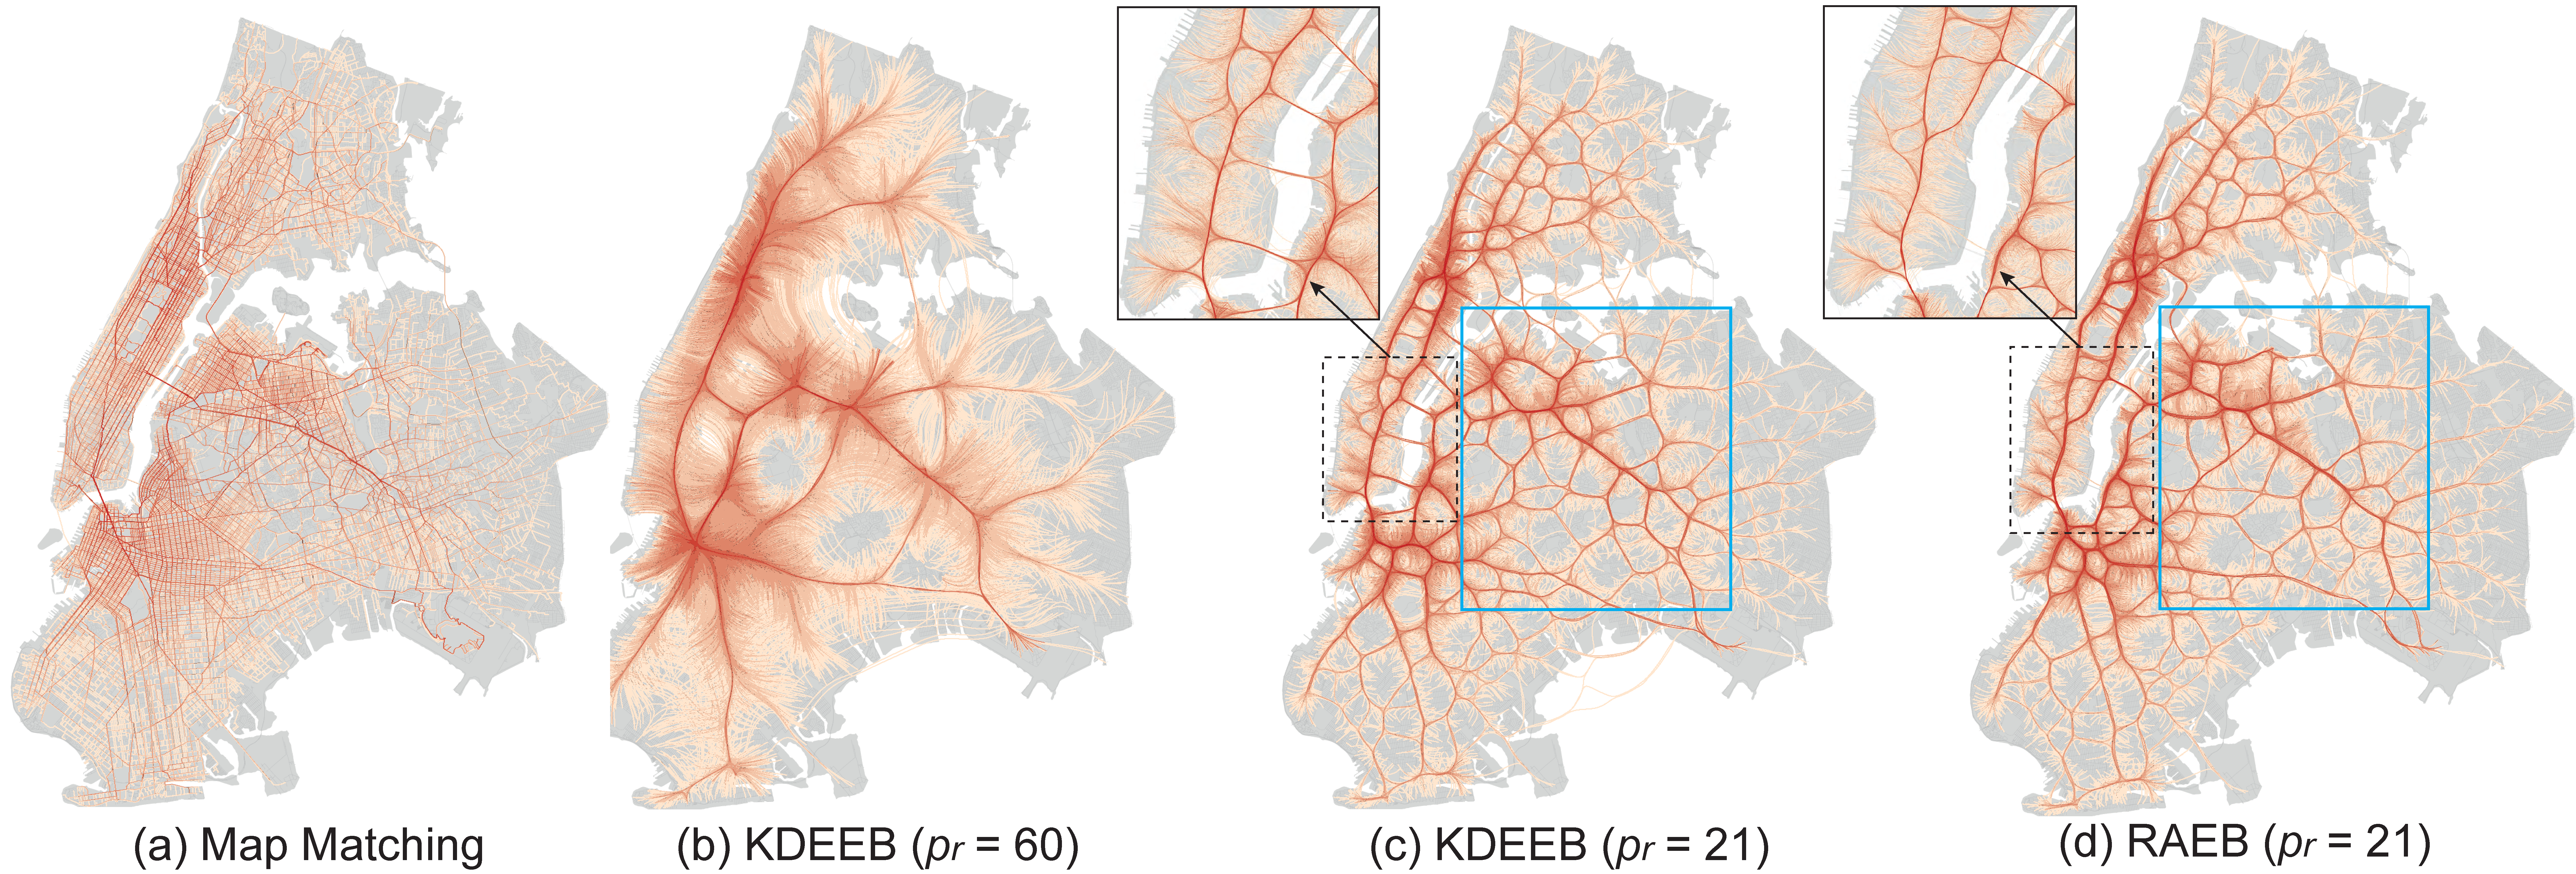
\includegraphics[width=0.995\textwidth]{figure/edgebundling/fig8_study2/NYC}
	\vspace{-2mm}
	\caption{Density maps of NYC taxi trips:
	(a) shortest paths mapped onto the road network, 
	(b) KDEEB bundles with kernel size $p_r$ = 60,
	(c) KDEEB bundles with $p_r$ = 21,
	and (d) our RAEB bundles with $p_r$ = 21.}
	\label{fig:nyc_visual}
	\vspace{-4mm}
\end{figure*}

\begin{figure}[t]
	\centering
	\includegraphics[width=0.45\textwidth]{figure/edgebundling/fig9_study2-2/NYC-zoom}
	\vspace{-3mm}
	\caption{Fine scale density maps of NYC taxi trips in Queens zone generated by (a) KDEEB, and (b) RAEB.}
	\label{fig:nyc-zoom}
	\vspace{-4mm}
\end{figure}

%%%%%%%%%%%%%%%%%%%%%%%%%%%%%%%%%%%%%%%%%%%%%%%%%%%%%%%%%%%%%%%%%%%%%%%%%%%%%%%%%%%%
\subsection{Artificial OD Trails}
\label{ssec:study1}

Our first example uses a random graph with 100K OD trails, and $5 \times 5$ grid and hierarchical reference graphs to simulate conventional road networks.
Raw OD trials and corresponding road networks are shown in the leftmost figures of Figure~\ref{fig:grid} and Figure~\ref{fig:hier}.
The OD trails are first mapped to underlying road networks using shortest path algorithm, and then both road networks are divided into three hierarchies that are colored in red, blue and green, receptively.
In the last, we apply RAEB on the OD trails, with all graph drawing sizes set to 1280$\times$1280 and initial kernel sizes $p_r$ set to 60.

In advance of KDEEB, RAEB allows to preserve route awareness by controlling parameter $p_{ra}$.
To evaluate the effects of $p_{ra}$, we set $p_{ra}$ to 0 - 3, and apply RAEB to OD trails on the grid road network as shown in the leftmost figure of Figure~\ref{fig:grid}.
The results are shown in Figure~\ref{fig:grid} (a) - (d).
In (a), $p_{ra}$ is set to 0, i.e., no route awareness will be preserved.
In this case, RAEB should be equivalent to KDEEB with other parameters the same.
The proof is demonstrated in (a), which shows smooth bundles similar to those in the original KDEEB~\cite{hurter2012graph}.
To preserve level 1 routes, we set $p_{ra}$ to 1, and the result is shown in (b).
As expected, OD trails around the red lines are bundled together with bundles following red lines, while other OD trails are bundled with bundles spreading arbitrarily in the graph drawing.
More route awareness can be preserved as we increase $p_{ra}$ to 2 and 3, as shown in Figure~\ref{fig:grid} (c) \& (d).

More importantly, route awareness $p_{ra}$ can be used to preserve topology of underlying road network.
Figure~\ref{fig:hier} (right) shows bundling result of RAEB applied to OD trails on a hierarchical road network that is shown in Figure~\ref{fig:hier}(left).
Here, $p_{ra}$ is set to 2, such that to preserve both the red and blue lines.
It is clear that the resulting bundles follow the lines, making it easy to trace OD trails.
In contrast, KDEEB will generate the same result with that in Figure~\ref{fig:grid}(a), as the underlying road network information is not used.

\begin{figure*}[t]
	\centering
	\includegraphics[width=0.995\textwidth]{figure/edgebundling/fig10_study3/shenzhen}
	\vspace{-2mm}
	\caption{
	Density maps of Shenzhen taxi trips: (a) raw GPS records are mapped onto road network, (b) KDEEB bundles trips on close aterial roads together, while (c) RAEB preserves these roads. All lines are colored according to the OD directions.
	}
	\label{fig:shenzhen}
	\vspace{-4mm}
\end{figure*}

%%%%%%%%%%%%%%%%%%%%%%%%%%%%%%%%%%%%%%%%%%%%%%%%%%%%%%%%%%%%%%%%%%%%%%%%%%%%%%%%%%%%
\subsection{New York Taxi Trips}
\label{ssec:study2}

In reality, a road network is usually much more complex, and OD trails are more dynamic than the artificial ones.
In this experiment, we further compare RAEB with KDEEB using results generated from New York taxi trips.

The road network employed in this study is extracted from OpenStreetMap (OSM) within the boundary of Manhattan, Brooklyn, Queens, and Bronx zones, where most origins and destinations are located.
The raw network consists of 133,154 nodes, 166,122 edges, and it is simplified to 97,336 routes.
The OD trails studied in this experiment are 100K taxi trips extracted from one-month trip records.
The original records consist of various attributes for each trip, including vendor id, pickup \& dropoff times and positions, and fare amount, etc.
We use the pickup \& dropoff positions, and map it onto the road network using shortest path algorithm.
Figure~\ref{fig:nyc_visual}(a) presents a density map of the mapped taxi trips.

Figure~\ref{fig:nyc_visual}(b - d) show bundling results generated by KDEEB and RAEB, with graph drawing sizes set to 1080 $\times$ 1440.
The experiment is started with KDEEB recommended settings of kernel size $p_r$ = 60 (about 5\% of graph drawing size) and $p_n$ = 10.
Figure~\ref{fig:nyc_visual}(b) shows the bundling result, which clearly presents several main bundles.
The bundles reveal primary traffic movements over the whole city.
Yet in other ways, the results are heavily bundled, missing details of road network topology.
To show more details, we measure initial kernel size considering both graph drawing and geometric property of road network as described in Section~\ref{ssec:kernel_size}.
$p_r$ is reduced to 21.
Figure~\ref{fig:nyc_visual}(c) shows the corresponding KDEEB bundling results.
More bundles are formed, in line with arterial roads in New York.
However, there are many bundles lying by non-existing roads, as those shown in the highlighted region in-between Manhattan and Brooklyn.
This illustration can cause wrong impression of bridges connecting the zones.
Figure~\ref{fig:nyc_visual}(d) shows results generated by RAEB, with $p_r$ = 21 and route awareness $p_{ra}$ = 1.
The undesirable bundles are removed by our method.

Visualization of urban traffic should support multi-scale exploration $-$ an important characteristic for movement data visualization.
In the context of this work, a good edge bundling algorithm should provide smooth transitions of bundling results at different scales.
We further evaluate multi-scale exploration by zooming into the blue region in Queens zone as in Figure~\ref{fig:nyc_visual}(c) \& (d), and applying KDEEB and RAEB on the OD trails.
The fine scale bundling results are presented in Figure~\ref{fig:nyc-zoom}(a) \& (b), respectively.
More bundles are generated by both methods, as the same effect when zooming into maps.
However, it is difficult to visually match bundles in Figure~\ref{fig:nyc_visual}(c) with those in Figure~\ref{fig:nyc-zoom}(a).
In comparison, bundles in Figure~\ref{fig:nyc_visual}(d) can be more easily identified in Figure~\ref{fig:nyc-zoom}(d).

%%%%%%%%%%%%%%%%%%%%%%%%%%%%%%%%%%%%%%%%%%%%%%%%%%%%%%%%%%%%%%%%%%%%%%%%%%%%%%%%%%%%
\subsection{Shenzhen Taxi Trips}
\label{ssec:study3}

We further evaluate the performance of RAEB using taxi trips in Shenzhen, with road network extracted from OSM.
In total, there are 161K nodes and 177K edges, and the edges are simplified to 51K routes.
The OD trails are one-week taxi trip records.
Unlike New York taxi records with only origin and destination positions, Shenzhen's data contain a sequence of GPS positions recorded in every 20 seconds.
We clean and extract in total 50K taxi trips from the records.
The trips are further mapped onto the road network using ST-matching algorithm~\cite{lou_2009_map}.

Figure~\ref{fig:shenzhen}(a) presents a graph of the map matching results in the size of 2160$\times$1280.
The lines of a trip are colored according to direction from the trip's origin to destination.
The graph shows that most taxi trips are recorded in the southern region of Shenzhen, which borders on Hong Kong and is more developed than other regions.
The unevenly distributed taxi trips make it improper to use kernel size $p_r$ recommended by KDEEB, which is over 100 as 5\% of the graph drawing size.
Instead, our method suggests $p_r$ = 26, considering the road network topology as well.

Using this setting of $p_r$, both KDEEB and RAEB reaches stable states at iteration 8.
Figure~\ref{fig:shenzhen}(b) \& (c) show the corresponding results, respectively.
Both methods create smooth bundles in line with arterial roads in Shenzhen, indicating $p_r$ measured by our method is preferable.
Besides, nearly the same bundles are generated in regions other than south part, except that RAEB's result shows more details.
More dissimilar results are shown in the highlighted areas.
Expressways G4 and G107 lead traffic to Shenzhen airport in the left region, while Beihuan and Binhai avenues holds main traffic in the right one.
KDEEB merges OD trails passing these roads, while our method splits the bundles.
In short, RAEB generates results more similar to real-world scenarios.
\section{Discussion}
\label{sec:discussion}

The experiments demonstrate that RAEB outperforms KDEEB in visualizing OD trails in urban traffic data.
The first experiment with artificial data shows that the introduction of route awareness $p_{ra}$ in RAEB distinguishes grid and hierarchical network structures.
The second experiment presents the comparisons between KDEEB and RAEB using New York taxi data, which records only origin and destination positions. 
The results with different kernel size $p_{r}$ and in multi-scales indicate that, 
(1) $p_{r}$ should be measured based on not only graph drawing size, but also underlying road network topology;
and (2) RAEB supports better multi-scale exploration.
The robustness of RAEB is further demonstrated through the third experiment with Shenzhen taxi data, which records a sequence of GPS positions in every 20 seconds.

The advancements are achieved by parameter settings adopted in RAEB.
This section presents detailed discussion on the parameters, followed by performance comparison between RAEB and KDEEB. 
In the end, we discuss about generality and limitation issues.

%%%%%%%%%%%%%%%%%%%%%%%%%%%%%%%%%%%%%%%%%%%%%%%%%%%%%%%
\subsection{Parameters}
\label{ssec:parameters}

\begin{table}[t]
	\begin{tabularx}{0.90\textwidth}{|>{\hsize=0.23\hsize}X|
                              >{\hsize=0.23\hsize}X|
                              >{\hsize=0.4\hsize}X|}
	\hline
	\textbf{Parameters} & \textbf{KDEEB} & \textbf{RAEB} \\
	\hline \hline
	Route & $-$ & 0 - Number of road \\
	awareness ($p_{ra}$) & & hierarchies \\
	\hline
	Kernel size ($p_r$) & Graph drawing & Graph drawing and road network geometry \\
	\hline
	Bundling & 10 - 15 & $-$ \\
	iterations ($p_n$) &  &  \\
	\hline
	Bundling & $-$ & \textit{NMI} between images in \\
	stability ($p_{s}$) & & consecutive iterations \\
	
	\hline
	Bundling & $-$ & Average Frechet distance\\
	deviation ($p_{d}$) & &  of bundles to OD trails\\
	\hline
	\end{tabularx}
	\caption{Main parameter adaptions in RAEB, in comparison with these in KDEEB.}
	\label{tab:parameters}
\vspace{-6mm}
\end{table}

RAEB adapts and introduces new parameters to better visualize OD trails in urban traffic data.
Table~\ref{tab:parameters} presents an overview of these parameter settings in comparison with those in KDEEB.

\begin{itemize}

\item
\textbf{Route awareness ($p_{ra}$):}
An input graph for KDEEB is straight lines connecting end nodes directly.
As discussed in the first experiment with artificial OD trails, such an input graph cannot distinguish grid and hierarchical road networks.
Instead, we introduce route awareness parameter $p_{ra}$ to control layout of input graph.
The first experiment also shows that $p_{ra}$ can be manipulated to generate bundles representing levels of details of road network.
If $p_{ra}$ is set to zero, input graph will be straight lines and the results are the same with KDEEB;
if $p_{ra}$ is set to the highest number of road hierarchies, input graph will be OD trails in line with road network, and more roads can be preserved.

\vspace{1mm}
\item
\textbf{Kernel size ($p_{r}$):}
In the second experiment with New York taxi data, we show that the parameter kernel size $p_r$ can control bundling coarseness.
KDEEB computes $p_{r}$ as 5\% of graph drawing size, which will generate coarse bundles that can only reveal main traffic connections (Figure~\ref{fig:nyc_visual}(b)).
Instead, RAEB suggests $p_{r}$ should be measured based on both graph drawing size and road network geometry.
In this way, a smaller $p_{r}$ is generated, and fine bundles that reveal details of street networks are generated (Figure~\ref{fig:nyc_visual}(c) \& (d)).
The advantage of our approach is further demonstrated using Shenzhen taxi data, which exhibits imbalanced distribution of taxi trips in the city.

\vspace{1mm}
\item
\textbf{Bundling iteration ($p_{n}$):}
KDEEB presets bundling iteration $p_{n}$ to a fixed number in between 10 - 15, such that to terminate the bundling process.
The choice of a suitable $p_{n}$, however, needs much experience and varies among different people. 
Adjustments in other parameters may also require fitting of the parameter.
RAEB discards this subjective parameter.

\vspace{1mm}
\item
\textbf{Bundling stability $p_{s}$:}
Instead, RAEB introduces a new parameter $-$ bundling stability $p_{s}$, to control bundling process termination.
$p_{s}$ is measured as normalized mutual information (\textit{NMI}) between images generated in two consecutive bundling iterations.
\textit{NMI} is a common metric in image processing field, thus can be easily integrated.
When $p_{s}$ reaches a predefined threshold, which means that visually a stable structure is generated, the bundling process will be automatically terminated.


\vspace{1mm}
\item
\textbf{Bundling deviation $p_{d}$:}
While $p_{s}$ measures bundling stability of a bundling method, it still lacks a method to quantitatively compare multiple ones.
The parameter bundling deviation $p_{d}$ is introduced to fill the gap.
$p_{d}$ is measured as average Frechet distance of bundles to corresponding OD trails.
The measurement is widely employed in geographical science, and we compare KDEEB and RAEB regarding the parameter below.

\end{itemize}

Some of these parameters can be automatically computed, including $p_r$ and $p_d$, while settings of $p_{ra}$ and $p_{s}$ can be consistent across different input data.
From the experiments, we recommend 1 for $p_{ra}$ (corresponding to top 5\% ranked routes), and 75\% for $p_{s}$.

%%%%%%%%%%%%%%%%%%%%%%%%%%%%%%%%%%%%%%%%%%%%%%%%%%%%%%%
\subsection{Performance}

\begin{table}[!tb]
	\setlength\extrarowheight{2pt}
	\begin{tabularx}{0.95\textwidth}{|
							  >{\hsize=0.19\hsize}X|
                              >{\hsize=0.16\hsize}X|
                              >{\hsize=0.05\hsize}X|
                              >{\hsize=0.17\hsize}X|
                              >{\hsize=0.13\hsize}X|
                              >{\hsize=0.17\hsize}X|
                              >{\hsize=0.13\hsize}X|}
	\hline
	Graph & Edge & $p_n$ & \multicolumn{2}{c}{Time (sec.)} \vline & \multicolumn{2}{c}{Deviation (pixel)} \vline \\
	& Samples & & KDEEB & RAEB& KDEEB & RAEB \\
	\hline \hline
	Random (grid) & 4.6M & 13 & 40.3 & 50.7 & 18.37 & 12.58 \\ 
	\hline
	NewYork & 3.1M & 11 & 34.3 & 42.9 & 15.40 & 9.88 \\
	\hline
	Shenzhen & 1.3M & 8 & 13.8 & 22.8 & 13.71 & 10.53 \\
	\hline
	\end{tabularx}
	\caption{Statistics comparison of KDEEB and RAEB for datasets used in the experiments. }
	\label{tab:statistics}
\vspace{-6mm}
\end{table}

Table~\ref{tab:statistics} shows comparison of KDEEB and RAEB for the datasets used in the experiments.
Both methods are implemented in Java running on a MacBook Pro with a 3.1 GHz Core i7 and Radeon Pro 560 graphics.
We employ the same kernel size $p_r$ and bundling iterations $p_n$ measured by our approach for both methods.

KDEEB's bundling process include sampling, splatting, advecting and smoothing steps.
Bundling time for each iteration is mainly determined by number of edge samples and kernel size.
Since kernel size measured by our approach is generally smaller than that by KDEEB, bundling time is reduced. 
The total running times for KDEEB methods are comparable with those in the original work~\cite{hurter2012graph}.
RAEB requires an additional step of bundling stability measurement, which is determined by the graph drawing size.
This adds in a running time of less than 1 seconds in each iteration for all three experiments.
The measurement is computed in every bundling iteration, thus we can shorten time by reducing the measurement frequency.
All the steps can be further accelerated using GPU e.g. CUDA~\cite{van2016cubu}.

On the other side, bundles generated by our method are more close to OD trials, as revealed by comparison regarding bundling deviation. 
From the table, RAEB reduces about 1/3 deviations of those in KDEEB for artificial and New York taxi datasets. 
The improvement is smaller for Shenzhen taxi data, though graph drawing in Shenzhen experiment is bigger.
This is probably because taxi trips are concentrated in a small area in the south of Shenzhen.
Nevertheless, the result image by RAEB shows more improvements than that by KDEEB (Figure~\ref{fig:shenzhen}(c) vs (b)). 


%%%%%%%%%%%%%%%%%%%%%%%%%%%%%%%%%%%%%%%%%%%%%%%%%%%%%%%
\subsection{Applicability and Limitations}
\label{ssec:app}

The experiments have shown the applicability of RAEB for bundling and visualizing OD trails in urban traffic using real-world taxi data.
RAEB introduces new parameters of route awareness $p_{ra}$ and bundling deviation $p_d$, and adapts existing measurement of kernel size $p_r$, to better fit road network topology.
The approach can be extended to other types of urban traffic data, such as commuter trips using public transportation, or people traces derived from call detail records.
These dataset consists of both OD trails and underlying road network.
Through advanced map matching algorithms, urban traffic's real paths on a road network can be recovered.
However, the parameters are not applicable to general graphs with information of only node connections, except for bundling stability $p_{bs}$.

Edge bundling methods face a common issue of unrealistic bundle lines.
Specifically for OD trails in urban traffic, bundle lines should not be far away from real paths.
RAEB mitigates the issue with route awareness $p_{ra}$ for controlling edge layout of input graph, and bundling stability $p_{bs}$ for generating stable results.
The first experiment shows that $p_{ra}$ can preserve certain routes on demand, while the second experiment reveals that RAEB supports better multi-scale exploration.
Experimental results of bundling deviations $p_{d}$ further proves the advantage of RAEB over KDEEB.
Nevertheless, these parameters can only constrain bundle layout in certain extent, as resulting bundle lines are still displaced from OD trials.
In scenarios requiring precise positions, such as query movements passing through a waypoint~\cite{kruger_trajectorylenses_2013} or road segment~\cite{wang_2014_visual-reasoning}, visual hints are required to remind the displacement.

Bundles generated by RAEB can show clear traffic patterns, meanwhile preserve road network topology better than KDEEB in a city.
These main goals of this work have been successfully achieved, as demonstrated by the experiments.
On the other hand, RAEB is not able to reveal detailed traffic patterns such as directional movements.
Direction is of recognized importance for studying OD trails in urban traffic~\cite{zeng_2015_visualizing}.
This limitation can be addressed by including directional information in density estimation or edge advecting functions, as described in CUBu~\cite{van2016cubu}.
Besides, RAEB is an image-based edge bundling method, constraining its applicability for 2D rendering only.
Applications such as to bundle movements~\cite{lambert20103d, thony2015vector} and fiber tracts~\cite{hurter_2018_functional} in 3D, and graphs in virtual reality~\cite{kwon_2016_study}, need spring- or geometry-based bundling methods.
\section{Conclusion and future work}
\label{sec:con}

OD visualization is challenging $-$ no universally good technique is available for visualizing arbitrary ODs~\cite{andrienko_visual_2012}.
In particular, this work studies OD trails in urban traffic.
We identify inconsiderate settings of existing kernel density estimation edge bundling (KDEEB) method when applied in the scenario.
This is because KDEEB was developed for general graphs such as airlines and migrations, while ignores data nature of urban traffic data.
These inconsiderate settings can cause domain-specific problems such as no preservation of road network topology and poor support of multi-scale exploration.
We contribute to the field with a new technique, namely route-aware edge bundling (RAEB). 
The bundling process is complemented with preprocessing that generate more proper input edge layout, and evaluation that create more stable visual results.
A series of parameter adaption and introduction are made to better cater to geometric properties of OD trails and road networks.
We compare RAEB with KDEEB in regarding to bundling time and deviation using artificial and real-world taxi data.
The experiment results show that RAEB outperforms KDEEB in reducing bundling deviation meanwhile achieving comparable computation speed.

Even though RAEB is specifically designed for bundling OD trails in urban traffic, some parameters such as bundling stability $p_{bs}$ can be applicable to other iterative edge bundling methods, including SBEB~\cite{ersoy2011skeleton} and FDEB~\cite{holten2009force}.
We would like to try integrating these parameters in the bundling methods, such that to make them more controllable.
We also realize many computation tasks in RAEB can be parallelized, thus bundling efficiency can be improved by GPU acceleration.
It would be worthy to reimplement RAEB in GPU, similar to CUBu~\cite{van2016cubu}.
Besides bundling control and efficiency issues, how to access bundling quality and faithfulness are the main challenges hindering the applicability of edge bundling methods~\cite{lhuillier2017state}.
Our experiences in developing RAEB suggest that in specific application scenarios, these challenges can be solved with domain knowledges.
On the basis of treating OD trails mapped onto road network as ground truth, our proposed parameter of bundling deviation $p_d$ is a quality and faithfulness metric in certain extent.
The parameters is derived from Frechet distance that is a common metric in geographical science.
In the future, we would like to apply RAEB in other fields such as to visualize neural connections in brain~\cite{2014_bottger_three-d, yang2016blockwise}.
Adaptions are most likely required, and we envision close collaborations with domain experts can facilitate the development.

% \chapter{Visual Interpretation of Recurrent Neural Network on Multi-dimensional Time-series Forecast}\label{chap:c3_intro}
Recent attempts at utilizing visual analytics to interpret Recurrent Neural Networks (RNNs) mainly focus on natural language processing (NLP) tasks that take symbolic sequences as input.
However, many real-world problems like environment pollution forecasting apply RNNs on sequences of multi-dimensional data where each dimension represents an individual feature with semantic meaning such as $PM_{2.5}$ and $SO_2$.
RNN interpretation on multi-dimensional sequences is challenging as users need to analyze what features are important at different time steps to better understand model behavior and gain trust in prediction.
This requires effective and scalable visualization methods to reveal the complex many-to-many relations between hidden units and features.
In this work, we propose a visual analytics system to interpret RNNs on multi-dimensional time-series forecasts.  
Specifically, to provide an overview to reveal the model mechanism, we propose a technique to estimate the hidden unit response by measuring how different feature selections affect the hidden unit output distribution. 
We then cluster the hidden units and features based on the response embedding vectors. 
Finally, we propose a visual analytics system which allows users to visually explore the model behavior from the global and individual levels.
We demonstrate the effectiveness of our approach with case studies using air pollutant forecast applications.


\chapter{Introduction}\label{chap:intro}
TBD
\input{chapter/4_MultiRNNExplorer/2_RelatedWork.tex}
\input{chapter/4_MultiRNNExplorer/3_RNN_Modeling_and_background.tex}
\input{chapter/4_MultiRNNExplorer/4_Analytics_Tasks.tex}
\input{chapter/4_MultiRNNExplorer/5_Model_interpreter.tex}
\section{Visualization Design}


In this section, we introduce the visual design based on the design tasks discussed in Sec.\ref{section:design_tasks}.  As shown in Fig.~\ref{fig:teaser}, the visual analytic system consists of six coordinated views. Starting from the configuration panel Fig.~\ref{fig:teaser}B, the users are able to select the target feature and the model to be analyzed. The region partition will be shown as Fig.~\ref{fig:teaser}B after the model is selected. To support exploring the model mechanism, the Cluster View is displayed to summarize the hidden units' response to the features (Fig.~\ref{fig:teaser}A) and the Feature Importance View (Fig.~\ref{fig:teaser}C) is shown to visualize the temporal importance of each feature. Furthermore, the users can select the individual cases in the Projection View (Fig.~\ref{fig:teaser}E) and all the selected individual cases are grouped by similarity and displayed in the Individual View (Fig.~\ref{fig:teaser}D).


\begin{figure}[t]
	\centering
	\includegraphics[width=0.95\textwidth]{figure/MultiRNNExplorer/teaser.pdf}
	\vspace{-3mm}
	\caption{Design of Hidden unit distribution and feature glyph. A) Hidden unit cluster; B) Hidden unit distribution; C) Feature cluster; D) Feature distribution for selected features; E) Feature glyph design; G) Response link MultiRNNExplorer contains multiple coordinated views to support exploring and understanding RNNs' behaviors on multi-dimensional time-series data, especially on hidden unit response and feature importance.
		The Configuration Panel (B) allows users to select a RNN models and configure parameters. 
		To reveal model mechanism, the Cluster View (A) summarizes the hidden unit clusters' response to feature clusters, and the Feature Importance View (C) summarizes the temporal importance of input features. 
		The Projection View (E) displays a data overview, allowing users to identify and select sequence instances of interest for further analysis. 
		The selected instances will be shown by the Individual View (D). }
	\label{fig:teaser}
	\vspace{-4mm}
\end{figure}
\input{chapter/4_MultiRNNExplorer/6_VIsualizationSections/ClusterView.tex}
\input{chapter/4_MultiRNNExplorer/6_VIsualizationSections/FeatureImportanceView.tex}
\input{chapter/4_MultiRNNExplorer/6_VIsualizationSections/ProjectionView.tex}
\input{chapter/4_MultiRNNExplorer/6_VIsualizationSections/SequenceView.tex}
\input{chapter/4_MultiRNNExplorer/6_VIsualizationSections/Interactions.tex}

\input{chapter/4_MultiRNNExplorer/7_Evaluation.tex}
\input{chapter/4_MultiRNNExplorer/8_Conclusion.tex}

\chapter{Conclusion and Future Work}

The fast increasing global urbanization process in recent years has greatly changed the world in the recent 50 years. The human migration from the rural area to the urban area results in a series of problems such as environment pollutant, traffic jam and insufficient local resource supply. Meanwhile, with the development of science and technology, a variety of data source can be collected easier and cheaper, which also provide the opportunity for analysts to understand the phenomenon and solve the problems. Although a lot of automatic techniques have been proposed in recent years, most of them still have limitations such as the lack of interpretability, difficulty in handling unexpected cases. Due to the variety of urban applications, these techniques always generate uncontrollable results which is hard to be accepted by the non-expert users. Thus the human experience and knowledge are required to make judgement or provide guidance in the analyzing process. Visual analytics, integrating the intuitive graphics and auto techniques, bridge the gap between users and complex urban data by taking human into the analysis loop.  

This proposal consists of three works that cover the three domains of urban information: place, people and technology. We start with a brief summary of the existing visualization techniques used in urban data exploration. After that, we introduced three visual analytics system target at the human-scale urban form exploration, large scale movement visualization and urban computing technique interpretation. 

In Chapter 2, we introduce Streetvizor, a framework enabling urban analysts to explore the human scale urban from city-, region- and street-level. The proposed system takes the street view images as input and extracts human-scale urban form features by leveraging the advanced machine learning techniques. Then, a visual analytics system is built upon the urban form feature database. The proposed method is evaluated by the real world data from four cities: London, Singapore, Hong Kong, and New York City. 

In Chapter 3, we have developed RAEB(route aware edge bundling), a novel edge bundling technique to visualize the overview of a large amount of OD trails in urban traffic data. Target at the limitation of traditional edge bundling techniques, we introduce the urban traffic network as a constraint to the trail bundles. A series of new parameters are employed in the pipeline.

In Chapter 4, we propose MultiRNNExplorer, a visual analytics system which helps analysts to understand the RNNs in high-dimensional time series forecast. The visual analytics system aims to interpret RNNs from two aspects, the overall model mechanism and the feature importance. Several case studies on air pollutant forecast show the effectiveness of the proposed technique.

Even though several novel designs and comprehensive analytics systems have been discussed in this proposal, the current development of urban related visualization techniques still cannot meet the analysis requirement due to the increasing complexity and variety of the applications. Based on the current work, we list several promising future directions.

\textbf{High-level urban analysis based on street view images.} In Chapter 2, we discuss how to leverage the easily collected street view images and advanced machine learning techniques to help us build the comprehensive visual analytics system for human-scale urban form explorations. In the future, we will extend the current framework to the more complex tasks. For example, an exiting research work uses vehicle classification techniques to estimate the demographic makeup of the US; We can also extract the signboards and building style from the street view images to support the exploration of urban region  functionalities.  

\textbf{Improve the bundling and rendering efficiency for the large trajectory dataset.} In Chapter 3, the edge bundling and rendering process still require tens of seconds to finish the visualization tasks, which makes the interactive exploration impossible. Our proposed technique is built upon the kernel density estimation techniques which can be parallelized. In the future, we will use the GPU-acceleration to improve bundling efficiency. In addition, to improve the computing efficiency, another strategy is to reduce the data amount. Traditional sampling methods, such as uniform and stratified sampling, cannot keep visualization accuracy. We plan to develop visualization aware sampling techniques to support the fast OD trails bundling. 

\textbf{Support model ensemble exploration.} Due to the complexity and variety of urban information exploration, a single forecast technique is always not enough to produce a credible and accurate result. In the future, we will extend the technique interpretation from RNNs to technique ensembles. However, use the same criteria to interpret multiple techniques is difficult due to the different algorithm mechanisms. Thus, we plan to figure out some uniform properties of these techniques (such as the feature importance) to make the them comparable. 


% \input{chapter/sec-introduction}
% \input{chapter/sec-related}
% \input{chapter/sec-design}
% \input{chapter/sec-implementation}
% \input{chapter/sec-hadoop}
% \input{chapter/sec-eval}
% \input{chapter/sec-conclusion}

%%%%%%%%%%%%%%%%%%%%%%%%%%%%%%%%%%%%%%%%%%%%%%%%%%%%%%%%%%%%%%%%%%%%%%%%%
%                                                                       %
%      9) BIBLIOGRAPHY                                                  %
%                                                                       %
% This example uses bibtex to generate the required Bibliography. Refer %
% to the % the file ustthesis_test.bib for the entries of the           %
% Bibliography. Note that only the cited entries are printed.           %
%                                                                       %
% If BibTeX is not used to typeset the bibliography, replace the        %
% following line with the \begin{thebibliography} and \end{bibliography}%
% commands (the "thebibliography" environment) to process the           %
% Bibliography.                                                         %
%                                                                       %
%%%%%%%%%%%%%%%%%%%%%%%%%%%%%%%%%%%%%%%%%%%%%%%%%%%%%%%%%%%%%%%%%%%%%%%%%

%%%%%%%%%%%%%%%%%%%%%%%%%%%%%%%%%%%%%%%%%%%%%%%%%%%%%%%%%%%%%%%%%%%%%%%%%
%                                                                       %
% The recommended bibliography style is the IEEE bibliography style.    %
% "ustbib" defines the IEEE bibliography standard with the added        %
% ability of sorting the items by name of author.                       %
%                                                                       %
% If you are not using BibTeX to process your Bibliography, comment out %
% the following line.                                                   %
%                                                                       %
%%%%%%%%%%%%%%%%%%%%%%%%%%%%%%%%%%%%%%%%%%%%%%%%%%%%%%%%%%%%%%%%%%%%%%%%%

\bibliographystyle{plain}

\bibliography{ref}
% Please run "bibtex ustthesis_test" before the bibliography can be
% included.

%%%%%%%%%%%%%%%%%%%%%%%%%%%%%%%%%%%%%%%%%%%%%%%%%%%%%%%%%%%%%%%%%%%%%%%%%
%                                                                       %
%     10) APPENDIX (If Any)                                              %
%                                                                       %
% \appendix command marks the beginning of the APPENDIX part of the     %
% Thesis. The usual \chapter command is used for the different chapters %
% of the Appendix.                                                      %
%                                                                       %
%%%%%%%%%%%%%%%%%%%%%%%%%%%%%%%%%%%%%%%%%%%%%%%%%%%%%%%%%%%%%%%%%%%%%%%%%


%%%%%%%%%%%%%%%%%%%%%%%%%%%%%%%%%%%%%%%%%%%%%%%%%%%%%%%%%%%%%%%%%%%%%%%%%
%                                                                       %
%     11) BIOGRAPHY (Optional)                                          %
%                                                                       %
% \biography and \endbiography are used to define the optional          %
% Biography of the author of the Thesis.                                %
%                                                                       %
%%%%%%%%%%%%%%%%%%%%%%%%%%%%%%%%%%%%%%%%%%%%%%%%%%%%%%%%%%%%%%%%%%%%%%%%%

% \biography
% The biography of the student is ALSO optional.
% \endbiography

\end{document}
